\lhead{\begin{tikzpicture}[remember picture, overlay]
    \node [anchor=100,inner sep=0] (imagenIZQUIERDA) at (current page header area.north){
\includegraphics[width=18cm]{img/Encabezado.PNG}};
    \end{tikzpicture}}
    \rhead{Piedra-Moreno}
    \rfoot{\begin{tikzpicture}[remember picture, overlay]
    \node [anchor=140,inner sep=0] (imagenDERECHA) at (current page footer area.south){
\includegraphics[width=18cm]{img/Foot.PNG}};
    \end{tikzpicture}}
    %----------------------------------------------------------------------------------------
    \lfoot{ \thepage}
    % \renewcommand{\labelenumi}{\alph{enumi}.)} 
    %----------------------------------------------------------------------------------------
    %----------------------------------------------------------------------------------------
    %	TITLE SECTION
    %----------------------------------------------------------------------------------------
    
    \setlength{\droptitle}{-5\baselineskip} % Move the title up
    \title{\textbf{Estudio de tiempos y movimientos en el ensamble de un circuito electrónico utilizando diferentes métodos para su optimización }} % Article title
    
     \author{ 
     \textsc{Piedra-Moreno, Alitza Alejandra}\\ 
     \texttt{ Instituto Tecnológico de Querétaro } \\ 
     \texttt{ Tecnológico Nacional de México } \\ 
     \texttt{Querétaro, México}\\ 
     \texttt{l22140912@queretaro.tecnm.mx} 
     \and 
     \textsc{Ángeles-Hurtado, Luis Alberto}\\ 
    %  Afiliación:
     \texttt{ Instituto Tecnológico de Querétaro } \\ 
     \texttt{ Tecnológico Nacional de México } \\ 
     \texttt{Querétaro, México}\\ 
     \texttt{alb3rt0.ah@gmail.com} 
    }
    
    
    %----------------------------------------------------------------------------------------
    
    % \begin{document}
    
    % Print the title
    \maketitle
    \thispagestyle{fancy}
    
    %----------------------------------------------------------------------------------------
    %	ARTICLE CONTENTS
    %----------------------------------------------------------------------------------------
    
    % \section*{Resumen}
    % \textit{Palabras clave:}
    % El resumen (ancho de página) deberá contener entre 100 y 200 palabras tipo Adobe Devangari 11 puntos.
    
    \begin{abstract}
    \noindent 
    El resumen (ancho de página) deberá contener entre 100 y 200 palabras tipo Adobe Devangari 11 puntos.
    
    \end{abstract}
    % 
    % 
    \textbf{\textit{Palabras clave}}: {Estudio, análisis, tiempo, movimiento, estándar, empresa, industrial, operación, muestra}
    % \keywords{First keyword should be the corresponding to the research area according with the authors guide. Maximum of 6 keywords.}
    
    \section{Introducción}
    
    Mejorar los procesos es un desafío para cualquier empresa, ya que puede implicar invertir capital a la mejora, en nueva maquinaria y hasta para capacitación del personal y al esfuerzo para alcanzar estándares de calidad más competitivos y muy pocas veces este dinero es destinado al desarrollo de nuevas tecnologías. \cite{83520408}
    
    %ensambleaje
    
    En el contexto industrial, un ensamblaje está referido al proceso de unir o conectar múltiples componentes individuales para construir un producto final o una parte de un producto más grande. Este proceso implica la unión de piezas mediante diversos métodos.
    
    
    %ensamblaje electronico 
    El ensamblaje electrónico alude al proceso de unir y conectar componentes electrónicos individuales para crear un sistema electrónico funcional. Este proceso es indispensable en la fabricación de una amplia variedad de dispositivos electrónicos, desde teléfonos inteligentes y computadoras hasta dispositivos médicos y sistemas de control industrial.
    
    
    %circuito electronico 
    
    Así mismo, los circuitos electrónicos son parte fundamental en la industria moderna, facilitando a la automatización, el control, la eficiencia energética, el monitoreo en tiempo real, la calidad del producto, la innovación y la seguridad laboral. Su importancia es tal que, sin ellos, muchas operaciones industriales se volverían aún más complejas, costosas o simplemente imposibles de realizar. En general, el ensamble de un circuito electrónico es un proceso complejo que involucra múltiples etapas, desde la selección y adquisición de componentes hasta la soldadura y pruebas finales. Para optimizar este proceso, se pueden emplear diversos métodos y estrategias, dentro de los cuales se encuentran el estudio de movimientos y tiempos, el estudio de tiempos predeterminados, el muestreo del trabajo, balanceo de líneas, datos estándar, entre otros.
    
    
    %Definicion de estudio de timepos y movimientos
    El estudio de movimientos y tiempos, está definido como el análisis de los movimientos, herramientas, materiales, e instalaciones utilizadas y que se han de utilizar, teniendo como objetivo encontrar la forma más económica de realizar el trabajo, normalizar los métodos, materiales, herramientas e instalaciones, determinar el tiempo estándar y ayudar al aprendizaje de los métodos. Con esto en mente podemos inferir que su objetivo es la optimización, que en otras palabras, busca las herramientas para que el proceso se ejecute en el mejor tiempo posible, que ofrezca mejores resultados y que economice, o de forma más simple, obtener los mejores resultados posibles de manera eficaz y eficiente  \cite{RAE}. Actualmente, en las empresas u organizaciones, sin importar su tamaño e industria, enfrentan enormes desafíos que les exigen ser competitivas en el mercado globalizado, la productividad de las empresas se ve más afectada por la distribución y relaciones de las plantas, entre diferentes sectores empresariales.
    
    %estudio de movimientos
    Un método de los que se habla en este documento es el estudio de movimientos, que es el análisis cuidadoso de cada uno de los movimientos que se emplean y que se han de emplear para realizar una tarea o de otra forma identificar cada uno de los Therbligs utilizados y que se han de utilizar, lo cuales se comprenden como los 17 movimientos básicos divididos en eficientes e ineficientes. Con el objetivo de eliminar los innecesarios para obtener una mayor eficiencia, incluyendo la comprensión del factor humano, así como el conocimiento, las materiales herramientas e instalaciones. \cite{niebel1980ingenieria} 
    
    
    %Sistema de tiempos determinados
    Por otra parte, el sistema de tiempos predeterminados, está definido como el conjunto de reglas o principios con el fin de determinar y resolver con anticipación la secuencia de pasos o sucesos.\cite{RAE}. Así mismo, es importante destacar que los STP se fundamentan en la utilización de los Therbligs, los cuales proporcionan a cada uno de ellos un valor de tiempo, además de que se incursiona en la medición de distancias y métodos con el propósito de obtener un estándar. Por otro lado, se introduce la medición de distancias y métodos con el fin de obtener un estándar.
    
    %Muestreo del trabajo
    En adición a la optimización del ensamblaje, se emplea el método de muestreo del trabajo, el cual consiste en la creación de un método de muestreo, en el cual se seleccionarán las muestras más representativas y que sean de alta calidad, que describan de manera exacta las características de un conjunto de fenómenos, lo que nos permitirá predecir, deducir, inferir y sacar conclusiones de este ensamble, y lograr ser lo más preciso y exacto posible. Además, Para llevar a cabo este procedimiento, se requiere la utilización de diversos métodos probabilísticos y estadísticos para inferir o llegar una conclusión más cercana a la real.
    
    
    De manera similar, para obtener el tiempo de producción más preciso, se utiliza el índice de desempeño del operador basado en la experiencia, capacitación y juicio del analista para establecer y confirmar el tiempo de producción. A medida que el intervalo se acorta, el intervalo de confianza disminuye. Con esto en mente tenemos el propósito de crear estos modelos, cuáles son los riesgos y estadísticas en los que nos enfocamos, cuál es el método de límite central que produce el promedio, que nos permite determinar en qué momento y horario estándar. Ayuda a proporcionar información más precisa durante el horario de funcionamiento estándar, proporciona una visión más clara de la base y mejora los procesos, recursos, distribución e instalaciones.
    
    %Balanceo de lineas
    Otro de los métodos que se pueden utilizar es el balanceo de líneas que es una herramienta muy útil para el control de la producción de una industria, dado que una línea de fabricación equilibrada permite la optimización de variables que afectan la productividad de un proceso tales como: inventarios de productos en proceso, los tiempos de fabricación y las entregas parciales de producción. El objetivo principal por el cual se realiza un balanceo de línea corresponde a la igualación de los tiempos de trabajo en todas las estaciones del proceso y el incremento de la eficiencia en general.\cite{‌Euroinnova}
    
    
    %estandares de trabajo 
    En contraparte, los estándares de trabajo que se calculan a partir de los datos y fórmulas estándar son relativamente consistentes, ya que los elementos calculados son el resultado de muchos estudios de tiempos probados con cronómetro. Como los valores están tabulados, solo es necesario sumar los elementos que se requieren para establecer un estándar, y todos los analistas deben llegar a estándares de desempeño idénticos para un método dado. Por lo tanto, se asegura la consistencia de los estándares establecidos por diferentes analistas en una planta, al igual que de los distintos estándares calculados por un determinado observador de estudio de tiempos. Por lo general, los estándares de un trabajo nuevo pueden calcularse con mayor rapidez mediante los datos o fórmulas estándar que a través de un estudio de tiempos con cronómetro. \cite{‌23}
    
    
    %Datos estandar 
    En la actualidad, cuando hablamos de datos estándar, nos referimos a todos los estándares de elementos tabulados, gráficas, nomogramas y tablas que permiten medir una tarea específica sin el empleo de un dispositivo medidor del tiempo, como un cronómetro. Los datos estándar pueden tener varios niveles de refinamiento: movimiento, elemento y tarea. Mientras más refinado sea el elemento del dato estándar, más amplio será su rango de uso. Por lo tanto, los datos estándar de movimiento tienen la mayor aplicación, pero toma más tiempo desarrollarlos que cualquier dato estándar de una tarea o un elemento. Una fórmula del estudio de tiempos es una presentación alternativa y, típicamente, más sencilla del dato estándar, en especial en el caso de los elementos variables. Las fórmulas tienen aplicaciones específicas en el trabajo no repetitivo, para el cual no es práctico establecer estándares para cada tarea con un estudio de tiempos individual. La construcción de una fórmula implica el diseño de una expresión algebraica que establece un tiempo estándar antes de la producción, sustituyendo valores conocidos propios de la tarea para los elementos variables.\cite{‌23}
    
    
    %Inteligencia artificial
    Actualmente, el sector de la fabricación ha experimentado avances importantes en la integración de inteligencia artificial para la mejora de un sinfín de operaciones. En este GRID de IA  hemos recogido el pulso de un buen número de organizaciones que trabajan en la integración de esta tecnología en los procesos de producción.
    
    En su mayoría, las voces de la industria proclaman la llegada de la IA a los dinámicos sistemas de producción como una fuerza impulsora clave que redefine los límites de la automatización y la robótica industrial. A medida que avanzamos hacia este futuro cercano, varios aspectos destacados de la IA están preparados para desempeñar un papel fundamental en la optimización y mejora de los procesos industriales. \cite{rouhiainen2018inteligencia}
    
    
    %Modelo y simulacion
    Como otro método que se puede utilizar tenemos la optimización industrial que toma el modelado y la simulación de procesos, como una herramienta fundamental para el estudio o análisis gráfico, físico o matemático de los procedimientos y actividades de un sistema de producción de una organización, con el fin de crear un nuevo diseño digital que automatice, optimice y logre la eficacia y la eficiencia de los procesos, suprimiendo errores y anticipando soluciones que alcancen en plenitud los objetivos de dicha organización.
    
    La simulación de procesos industriales permite esquematizar los procesos generando modelos virtuales donde se pueden identificar los errores, verificando el layout, anticipándose a los resultados de los procesos de producción de manera precisa y sin correr riesgos.
    
    Con el modelado y la simulación de procesos industriales podemos optimizar los tiempos de los procesos, examinando diferentes alternativas. Además, obtenemos la facultad de analizar las fases críticas de procesos como la ergonomía, la producción, el mantenimiento, la logística, la layout (disposición de medios), entre otros; acentuando la calidad y la precisión del diseño. Igualmente, se obtiene la supresión de costos extra, ya que se puede verificar, revisar y automatizar el diseño de optimización en tiempo real. \cite{sanchez2015analisis}
    
    Con todo esto en mente, resumimos que a través de todos estos métodos y teniendo en cuenta los avances en la industria para la optimización de los ensambles así como los métodos antiguos, los que se busca encontrar en este artículo es el diseño, mejora e integración de sistemas productivos aplicando todas etas tecnologías para una dicha optimización, mediante la mejora continua, el análisis y estandarización.
    
    
    \section{Justificación}
    
    La industria constituye la actividad más importante de la producción material en la mayoría de los países. Tal y como se conoce hoy, esta actividad se desarrolla a partir de la revolución industrial en Inglaterra y ha estado estrechamente ligada al progreso en los países capitalistas más avanzados.
    
    Durante la mayor parte de la centuria pasada, los economistas llegaron a establecer una conexión directa entre industrialización y desarrollo, fundamentalmente sobre la base de la experiencia de los países ricos y, luego, de la extinta Unión de Repúblicas Socialistas Soviéticas (URSS). Varios economistas destacados, como Rosenstein-Rodan (1943), Prebisch (1950), Lewis (1954), Hirschman (1958) y otros, le otorgaron un lugar central a la manufactura en el esfuerzo de desarrollo de los países más atrasados. Su valor se relacionó con la explotación de economías de escala junto a una alta y creciente productividad del trabajo; su papel, con la mejoría de los términos de intercambio, el acelerado cambio técnico y una gran capacidad de impactar en el avance de otras ramas a través de encadenamientos productivos. Kaldor (1966), por ejemplo, resaltó que estos elementos permitían explicar la presencia de rendimientos crecientes, lo que estaría detrás del colapso del crecimiento económico en estados industrializados que experimentaran una pérdida sostenida de su tejido industrial. 
    
    
    
    La mayoría de estos efectos se han manifestado claramente en la trayectoria de un grupo de nuevos países industrializados (NPI), esencialmente en Asia, pero también en el caso de Irlanda y Brasil. Un aspecto especialmente relevante tiene que ver con su impacto en el avance científico-técnico y en la innovación-desarrollo (I+D). Datos recientes (McKinsey Global Institute MGI, 2012) indican que más del 90 \% del gasto en I+D en el sector productivo se origina en la manufactura; mientras que las cinco revoluciones tecnológicas descritas hasta la actualidad han tenido como punto de partida la actividad industrial, para luego generar considerables externalidades hacia el conjunto del sistema económico.
    
    Estas consideraciones forman parte de la agenda de desarrollo para las naciones pobres. Por ello es indispensable conocer las tendencias más importantes del desarrollo industrial en el mundo y sus consecuencias para la formulación de políticas en este grupo de estados
    
    
    %competitividad
        En la actualidad, la competitividad de las empresas es considerada una cuestión fundamental en los sectores económicos tanto de los países desarrollados como en desarrollo. El contexto internacional y en especial el proceso de globalización requieren que las organizaciones cuenten con recursos eficaces y eficientes en la gestión de los recursos financieros, humanos, naturales y tecnológicos, entre otros, para afrontar el desafío del mercado, no solo nacional, sino fuera de las fronteras de sus países de origen. \cite{labarca2007consideraciones}
        
        En el nivel medio o marco, la competitividad está relacionada con las ventajas relativas de los recursos de un país o región, ya sea tierra, trabajo y capital, o con las ventajas que surgen principalmente de las inversiones en formación de capital humano e innovación. \cite{padilla2006instrumento}
        
        En la situación actual, donde prevalecen continuos y rápidos cambios tecnológicos, la formación juega un papel muy importante para fortalecer la competitividad de la empresa, como productora de capital humano. Por un lado, complementa la formación formal, proporcionando al empleado los conocimientos y habilidades necesarios para utilizar, adaptar y, en última instancia, mejorar la tecnología. Por otro lado, dado que tiene como objetivo proporcionar a los empleados los conocimientos y habilidades que necesitan en sus operaciones diarias, se puede esperar que genere un retorno rápido y significativo para la empresa.\cite{casar1993competitividad}
        
        Desde comienzos de año, diversos indicadores muestran una clara divergencia entre la actividad del sector manufacturero y el sector servicios. De hecho, según los índices PMI globales, la actividad manufacturera se está enfriando desde inicios del pasado año (y se encuentra ya estancada o en retroceso en algunos países), mientras que el sector servicios ha mostrado una notable recuperación.
        
        Parte de esta divergencia entre manufacturas y servicios responde a su diferente naturaleza cíclica. El consumo de bienes duraderos y la producción manufacturera son muy cíclicos y sensibles a cambios en las condiciones monetarias. Por tanto, es lógico pensar que la notable tensión experimentada por las condiciones monetarias globales desde comienzos de 2022 ha terminado enfriando la actividad en el sector industrial. Sin embargo, existen otros motivos que explican que la discrepancia sectorial actual se encuentre en máximos desde la crisis financiera de 2008. \cite{CaixaBank}
    
        Dentro de la industria manufacturera se pueden destacar 4 formas distintas de producción. La cuales se encuentra la manufactura repetitiva, la manufactura discreta, la manufactura continua y la manufactura por lotes. Donde la mayoría de las empresas utilizan más de uno de estos procesos para obtener un producto. \cite{JavierA}
        
    %indistria 4.0
        Por otra parte, la Industria 4.0 se define como la integración de tecnologías digitales inteligentes dentro de la fabricación y los procesos industriales. Tomando en cuenta las tecnologías que incluyen redes industriales de IoT, IA, Big Data, robótica y automatización. Así mismo, la Industria 4.0 permite la fabricación inteligente y la creación de fábricas inteligentes. Con esto, su objetivo es mejorar la productividad, la eficiencia y la flexibilidad, de forma que posibilita una toma de decisiones y una personalización más inteligentes en las operaciones de fabricación y de cadena de suministro. \cite{SAP}
    
       %cuantas industrias de manufactura existen en el mundo
    
    A ciencia cierta, el determinar el número de industrias o establecimientos existentes en el mundo es muy complicado, ya que este número puede variar dependiendo de cómo se clasifiquen y cuántos sectores se incluyan, además que la manufactura abarca una gran cantidad de actividades. Debido a todo esto es imposible dar un número en concreto, pero para tener en cuanta su impacto, el Banco Mundial nos proporciona una lista Valúa el valor agregado de la manufactura en cada país, y nos proporciona una gráfica donde nos engloba el valor agregado de la manufactura en todo el mundo la cual es de 16.19 trillones de dólares,
    
     %cuantas industrias de manufactura existen en mexico 
      
    Cabe mencionar a  los datos últimos datos registrados en diciembre de 2023, muestra que México contaba con 611.331 establecimientos relacionados con el sector manufacturero. Siendo el Estado de México la entidad federativa con la mayor cantidad de locales de este tipo, albergando cerca del 11\% del total. Le siguieron Oaxaca y Jalisco, ambos estados con más de 53.000 establecimientos en esta industria. Así mismo, a nivel nacional, en 2018 hay 6,493,020 personas que trabajan en esta industria.
    
    Comparada con otros sectores de la economía, la manufactura ocupa el tercer lugar por el número de personas que trabajan en ella; en esta industria, el número de hombres es mayor que el de mujeres.
    %cuantas industrias de manufactura existen en queretaro  
    Actualmente, en Querétaro existen 7,649 establecimientos dedicados a las manufacturas, siendo así Querétaro es uno de los estados con el mayor número de parques industriales del país, donde están asentadas empresas mexicanas, estadounidenses, alemanas, canadienses y coreanas.
       
    %parques industriales en queretaro    
        
        El sector industrial en el estado de Querétaro, aporta el 36 por ciento de los empleos totales en la entidad. Es decir, hay 352 mil puestos laborales en este sector. Esto debido a que se tiene un total de 49 parques industriales en la entidad.
        
        Querétaro se ha destacado a lo largo de los años por su notable crecimiento económico y por mantenerse en los primeros lugares dentro de los indicadores de actividad económica. Este significativo desarrollo económico e industrial se refleja en que Querétaro es de los estados con mayor número de parques industriales del país. \cite{JessicaIgnot}
        
        En el estado se tiene registro de 67 parques y zonas industriales, que se concentran principalmente en El Marqués (34.3\%), Querétaro (31.1\%), Colón (13.4\%); los restantes están en Pedro Escobedo, Huimilpan, Corregidora y Cadereyta (20.9\%), expone el Anuario Económico Estatal, edición 2021, de la Secretaría de Desarrollo Sustentable.
    
    % 
    % 
    \section{Descripción del problema}
    
    El problema de optimización del ensamble electrónico es multifacético y requiere un enfoque integral que tenga en cuenta la eficiencia, los costos, la calidad, la flexibilidad y la tecnología. Al utilizar varios métodos y enfoques, las empresas pueden mejorar la eficiencia y la competitividad de sus operaciones de ensamble electrónico en un mercado cada vez más exigente.
    
    Otro de los problemas que encontramos en este estudio es que al utilizar el método de muestreo, se reducirán los costos, pero el problema será encontrar una muestra que sea representativa de la población, así como encontrar el valor esperado real y la variación de nuestros datos.
    
    Otro de los problemas que nos hemos de encontrar será el sacar el tiempo ciclo así como el buen análisis de tiempo productivo además que al usar el método de sistemas de tiempos predeterminados el juicio del analista sea el correcto, ya que este puede variar entre analista y no suele ser el más preciso y exacto.
    
    Por otra parte, una de nuestras incógnitas científicas es el tiempo ciclo, que es el que en nuestro estudio es el primer elemento a sacar para el inicio de nuestro análisis. Así mismo describimos el problema como la baja productividad y eficiencia que contenemos en nuestro ensamblaje, por ello mesmo debemos buscar un método en el cual nuestro circuito eléctrico pase de un elemento inestable con el movimiento, difícil de identificar las partes, costoso y desordenado a un elemento de fácil manejo, identificación simple de los elementos, simpleza de los pasos para los empleados y un costo menor, el cual será un gran beneficio para la empresa. 
    
    También contamos con la incógnita de si el método probabilístico será el correcto, ya que al final solo son suposiciones, por lo que se espera que el valor obtenido sea el más cercano, mientras que nuestros datos sean los correctos.
    
    \section{Fundamentación teórica}
    
    Los términos estudio de tiempos y estudio de movimientos fue creado por W. Taylor y Frank B. Gilbert y su esposa Lilian M. El estudio de movimientos y tiempos implica el análisis de movimientos, herramientas, materiales e instalaciones utilizadas y que se han de utilizar y consta de 4 etapas:
    \begin{enumerate}
        \item Encontrar la forma más económica de hacer el trabajo.
        \item Normalizar los métodos, materiales, herramientas e instalaciones usadas.
        \item Determinar exactamente el tiempo necesario para que una persona completamente capacitada realice el trabajo con una marcha normal.
    \item Ayudar al aprendizaje del operario en el método nuevo.
    \end{enumerate}
    
    Por otra parte, el estudio de movimientos implica el análisis cuidadoso de cada uno de los movimientos corporales que se emplean para realizar una tarea, con el fin de eliminar los necesarios para obtener la máxima eficiencia, incluye la comprensión del factor humano así como el conocimiento de los materiales, herramientas e instalaciones. 
    \cite{niebel1980ingenieria}
    
    
    Para esto se debe conocer los movientes básicos, ya que los Gilbreth concluyeron que todo trabajo, ya sea productivo o no, se realiza mediante el uso de combinaciones de 17 movimientos básicos a los que ellos llamaron therblig \cite{niebel1980ingenieria}  
    
    Estos se dividen en eficientes, que estimulan el progreso del trabajo y con frecuencia pueden ser acortados, pero por lo general no pueden ser eliminados:
    \begin{enumerate}
        \item \textbf{Alcanzar (AL):} “Mover” la mano vacía hacia o desde el objeto; donde el tiempo depende de la distancia recorrida.
        \item \textbf{Mover (M):} “Mover” la mano cargada; el tiempo depende de la distancia, el peso y el tipo de movimiento.
        \item \textbf{Tomar (T):} “Cerrar” los dedos alrededor de un objeto, este comienza cuando los dedos tocan el objeto y termina cuando se ha ganado el control.
        \item \textbf{Soltar (SL):} “Soltar” el control de un objeto, normalmente el más corto de los therbligs.
        \item \textbf{Preposicionar (PP):} ”Posicionar” un objeto en una ubicación predeterminada para su uso posterior. Por lo general ocurre en conjunto con “Mover”.
        \item \textbf{Utilizar (U):} “Manipular” Una herramienta para el uso por el que fue diseñada; fácilmente detectable a medida que avanza el progreso del trabajo.
        \item \textbf{Ensamblar (E):} “Unir” dos partes que embonan. Por lo general es precedido por “Posicionar” o “Mover” y seguido por “Liberar”.
        \item \textbf{Desensamblar (DE):} Es lo opuesto a “Ensamblar”, pues separa partes que embonan.
    
     También encontramos los ineficientes, los cuales no representan un avance en el proceso del trabajo y debe eliminarse. En esta categoría encontraremos:
    
        \item \textbf{Buscar (B):} Ojos o manos buscan un objeto; comienza a medida que los ojos se mueven para localizar un objeto.
        \item \textbf{Seleccionar (SE):} “Mover” la mano cargada; el tiempo depende de la distancia. Por lo general es seguido por “Buscar”.
        \item \textbf{Sostener (SO):} Una mano soporta el objeto mientras la otra realiza trabajo útil.
        \item \textbf{Posicionar (P):} “Orientar” un objeto durante el trabajo, por lo general precedido por “Mover” y seguido por “liberar”.
        \item \textbf{Inspeccionar (I):} “Comparar” un objeto con el estándar, típicamente a la vista, pero podría ser también con los demás sentidos.
        \item \textbf{Planear (PL):} “Pausar” para determinar la acción siguiente; por lo general se le detecta como un titubeo que precede a “Mover”
        \item \textbf{Retraso Inevitable (DI):} Más allá del control de quien opera debido a la naturaleza de la operación.
        \item \textbf{Retraso Evitable (DEV):} Quien opera es único/a responsable del tiempo ocio.
        \item \textbf{Descansar (DES):} Aparece periódicamente, no en cada ciclo. Depende de la carga de trabajo física.
    
    \end{enumerate}
    
    De la misma manera se considera el sistema de tiempos predeterminados (STP) los cuales son un conjunto de reglas o métodos para determinar con anticipación la secuencia de sucesos. Este está basado en los anteriormente mencionados Therbligs, ya que a estos elementos les asignaron valores de tiempo, aunque ciertamente los STP “no siempre pueden predecir con precisión” el tiempo que le lleva a un trabajador realizar una tarea. Uno de los problemas de este método es que no son automáticos, es decir, que requiere del juicio del analista. Y esto se menciona, ya que cada analista obtiene tiempos distintos para un mismo trabajo porque interpretan las reglas en forma diversa. Así mismo en los STP lo que mediremos será la distancia, así como los métodos, ya que estos nos ayudaran a estimar el tiempo estándar que nos llevara realizar una tarea. 
    
    
    
    En consiguiente, él métodos de medición del tiempo es un sistema estandarizado para medir los tiempos que tardan los trabajadores en ejecutar una tarea repetitiva. El objetivo de este sistema es analizar donde están los movimientos ineficaces que se traducen en pérdidas innecesarias de tiempo en una tarea que se ejecuta cientos de veces al día. \cite{DanielGrifol}
    
    Cabe resaltar que para hablar de estos métodos debemos describir lo que es la precisión y la exactitud, donde la precisión es lograr la mínima dispersión al momento de hacer una medición o de realizar una tarea. Es la variación o poca variación significa un buen grado de precisión. Y la exactitud se define con respecto a su cercanía o sesgo, mayor cercanía implica un buen grado de exactitud.
    
    Retomando el tema, el muestreo es la acción de escoger muestras representativas de calidad que describa de manera exacta las características de un conjunto que nos dejen deducir, inferir y sacar conclusiones de un fenómeno a estudiar. \cite{RAE} Teniendo en cuanta qué representativo alude a lo significativo, característico, peculiar, relevante e importante. \cite{RAE}
    Por ende, el muestreo de trabajo lo podemos considerar como una herramienta para disminuir el costo que se presenta  en el estudio continuo del tiempo. Su único problema es obtener una muestra representativa. Así mismo, utilizando el muestreo del trabajo, reducimos el costo que implica un estudio de tiempos convencional, pero surge el problema de obtener una muestra representativa.
    
    Teniendo en cuenta que el estudio de tiempos convencional, es una muestra continua de n ciclos, suponiendo que la distribución estadística es normal y el estudio de tiempos no convencional contiene huecos entre las lecturas de muestreo y es una muestra discreta suponiendo que la distribución estadística es binomial.
    
    
    Así mismo se utilizará lo conocido como el tiempo productivo, que es la calificación del desempeño de operador, está basada en la experiencia, capacitación y juicio del analista que lo realiza.
    
    
    Con esto en mente en nuestro estudio utilizaremos diversas herramientas como lo es el diagrama de movimientos bimanual la cual es una herramienta que muestra todos los movimientos y retrasos atribuibles a las manos derecha e izquierda, además de la relación que existe entre ellas. Tiene como propósito identificar los patrones de movimiento que resultan ineficientes y observar las violaciones a los principios de la economía de movimientos.\cite{niebel1980ingenieria} Así mismo, el equipo mínimo requerido para realizar un programa de estudio de tiempos incluye un cronómetro, un tablero de estudio de tiempos, las formas para el estudio y una calculadora de bolsillo. Un equipo de videograbación también puede ser muy útil.
    
    
    En donde en una forma de estudios se registra toda la información pertinente sobre el método que se estudia, las herramientas utilizadas, etc. La operación en estudio se identifica mediante información como nombre y número del operario, descripción y número de la operación, nombre y número de la máquina, herramientas especiales usadas y sus números respectivos, el departamento donde se realiza la operación y las condiciones de trabajo prevalecientes. 
    \cite{niebel1980ingenieria}
    
    Por otra parte, una de las mayores incógnitas que nos surgen será el de cuantos ciclos de estudio deberemos implementar, como el estudio de tiempos es un procedimiento de muestreo, se puede suponer que las observaciones se distribuyen normalmente respecto a una media poblacional desconocida con una varianza desconocida. Si se usa la media muestral y la desviación estándar muestral s, la distribución normal para una muestra grande lleva al siguiente intervalo de confianza \ref{equ:1}. 
    
    \begin{equation}
        \label{equ:1}
        x {\pm} {\frac{zs}{\sqrt{n}}}
    \end{equation}
    
    Pero esto claramente suponiendo que fuera una muestra grande, pero en nuestro caso se entiende que nuestra muestra será menor a 30 por ende se deberá utilizar el método de la T, pero primeramente a falta de tiempo se utilizara el método probabilístico en donde contaremos en el teorema del límite central.
    
    En donde comprendemos al límite central como la exposición y descripción de datos de un fenómeno, y se comprende de verdades admitidas sin demostración, que sirven como base para posteriores razonamientos lógicos y que permiten aproximar magnitudes mediante la secuencia de números, estimando la tendencia central y dispersión de los parámetros. \cite{RAE}
    
    
    
     La "5S" es una metodología de organización en el lugar de trabajo que se originó en Japón. Representa cinco palabras japonesas: Seiri, Seiton, Seiso, Seiketsu y Shitsuke, que se traducen al español como Clasificar, Ordenar, Limpiar, Estandarizar y Mantener en español. La metodología 5S tiene como objetivo mejorar la eficiencia, la seguridad y la productividad al organizar el lugar de trabajo, eliminar desperdicios y mantener la limpieza. A menudo se utiliza en entornos de fabricación, servicios y oficinas para optimizar procesos y crear un espacio de trabajo más organizado y eficiente.
    
     Cada una de esta 5 etapas consiste en diferentes estrategias, y son dependiente en cadena, por ello mismo se debe tener en cuenta su concepto y estos  son los siguientes:
    
    CLASIFICACIÓN (SEIRI):
    
    Consiste en identificar y clasificar los materiales indispensables para la ejecución del proceso. El resto, se considerará material innecesario y, por lo tanto, se eliminará o separará. A partir de ese momento, se realizará un inventario estándar de cada puesto de trabajo.
    
    De esta forma, el trabajador dispone de las herramientas que realmente necesita y ya no existirán otros elementos que puedan dificultar su trabajo.
    
    ORGANIZACIÓN (SEITON):
    En segundo lugar, se procede a ordenar los materiales indispensables, facilitando las tareas de encontrar, usar y reponer estos útiles.
    
    Con ello se consigue eliminar tiempos no productivos asociados a la búsqueda de materiales y desplazamientos innecesarios. Se debe marcar la ubicación de cada material, componente o herramienta, para ello nos servimos de etiquetas, moldes, dibujos, señales, etc.
    
    LIMPIEZA (SEISO):
    Es indispensable localizar y eliminar la suciedad del puesto de trabajo, así como su correcto mantenimiento.
    
    Disponer de un estándar adecuado de limpieza y organización repercute directamente en la motivación del personal, además de reducir en gran medida los accidentes y lesiones.
    
    ESTANDARIZAR (SEIKETSU):
    El proceso de estandarizar trata de distinguir fácilmente una situación “normal” de una “anormal”, es decir, el personal debe ser capaz de discernir cuando las tres eses anteriores se están aplicando correctamente y cuando no.
    
    Es imprescindible que todo el personal de planta disponga de la formación adecuada para identificar este tipo de situaciones. De esta forma, el personal se siente más valorado y aumenta su motivación. A su vez, los operarios son más polivalentes y son capaces de detectar pequeños fallos en su puesto, que a posteriori pudieran desencadenar problemas más graves.
    
    SEGUIR MEJORANDO (SHITSUKE):
    Las 5S no tienen un fin definido. Es un ciclo que se repite continuamente y en el que se debe de disponer de una disciplina para mantener un puesto de trabajo ordenado y limpio.
    
    El éxito en la implantación de las 5S, genera un espacio de trabajo mucho más agradable, se reducen stocks, accidentes y se aumenta la productividad y satisfacción del personal de la empresa. Por ello la prioridad es mantener esta disciplina de una forma rigurosa y constante.
    \cite{justo}
    
    
    
    
    
    
    \section{Hipótesis}
    
    Al momento del desarrollo de nuestra optimización, se generarán diversas cuestiones acerca del cómo se debe hacer, cuál es el método adecuado, si lo estamos haciendo correctamente, entre otras. Por ello, se debe prevenir estos problemas con anticipación y generar una hipótesis que nos ayude a trabajar y destacar en los problemas que se deben utilizar.
    
    Al comienzo de nuestro trabajo, tendremos el problema de identificar correctamente las partes de los materiales, pero a medida que avancemos en el desarrollo de la práctica, podremos generar un mayor conocimiento de estos, que nos ayudará a desempeñarnos más en el ensamble y su optimización.
    Otra cuestión, el escaso conocimiento de los métodos de ensamblaje de los circuitos, los cuales, sin duda, existen diferentes, como la impresión 3D, el uso de robots y hasta el uso de inteligencia artificial. Aunque no dispongamos de todas esas tecnologías, tendremos un buen desarrollo de la optimización, ya que contamos con conocimientos recabados y un buen razonamiento.
    
    
    \section{Objetivo}
    
    Diseñar, mejorar e integrar sistemas productivos de bienes aplicando tecnologías para su optimización. Diseñar, implementar y mejorar sistemas de trabajo para evaluar la productividad. Analizar, los movimientos, herramientas, materiales e instalaciones utilizadas y que se han de utilizar para encontrar la forma más económica de hacer, el trabajo. Normalizar los métodos, materiales, herramientas e instalaciones, utilizadas y que se han de utilizar. Determinar el tiempo necesario y estándar de realización del trabajo.
    
    
    \subsection{Objetivos específicos}
    
    \begin{itemize}
        \item Identificar los materiales, describirlos, recaudar información de ellos, estandarizarlos y normalizarlos.
        \item Crear una secuencia de pasos para estandarizar los procedimientos a realizar en el ensamblaje.
        \item Dividir las operaciones en elementos, para posterior identificar y eliminar los movimientos ineficientes.
        \item Generar un muestro de calidad, y que sea representativo para la toma de tiempos.
        
        \item Obtener la media muestral y la desviación estándar para estimar lo que es conocido como la media poblacional y la variancia de nuestros tiempos.
        \item Obtener una aproximación al tiempo estándar de la operación.
        \item Conseguir el tiempo siclo y estándar del ensamble de nuestro circuito electrónico.
        \item Realizar un plan de emergencia para la empresa.
        
    \end{itemize}
    
    % 
    % \section{Cuerpo }
    
    \section{Metodología}
    \subsection{Desarrollo de la guía de plan de Emergencia}
    
    El Plan de Emergencia: Documento que describe los lineamientos a seguir, la organización y los mecanismos, que indican la manera de enfrentar una situación de emergencia o desastre, tanto en lo general como en lo particular, así como la utilización viable de los recursos humanos y materiales con los que se cuenta.
    % 
    % 
    \subsection{Análisis de los métodos, materiales, herramientas e instalación utilizada en la ejecución del ensamble de un circuito electrónico}
    
    \subsubsection{Planeación}
    
    Asegúrate de conocer siempre tu objetivo.
    Asegúrate de contar con los documentos (formatos, procedimientos, etc).
    % 
    % 
    
    En el desarrollo de nuestra práctica es indispensable conocer cada una de las partes de nuestro ensamble esto a raíz de que como operario nos es mucho más simple realizar nuestro trabajo si uno conoce y/o se familiariza con cada pieza que se utiliza además que como analista nuestro trabajo es examinar cada parte, medida y hasta material que está implícito en el trabajo para generar una mejora en nuestro método y a su vez implementar el objetivo del estudio del trabajo que es encontrar una forma más económica así como la estandarización de las herramientas, materiales e instalaciones, por ello mismo se debe en listar cada parte del ensamblaje para que a la hora del desarrollo del estudio tengamos una secuencia con orden.
    
    En el apéndice \ref{Figura:Materiales} se muestra cada una de las partes de nuestro ensamble, así como su número de pieza, figura de solidworks y precio.
    
    Con este orden establecido pasaremos a desglosar cada una de las características de nuestras piezas para conocerlas de mejor forma, así como generar  el diagrama y dibujo de cada una de ellas.
    
    \subsubsection{PC-01: Tapete profesional organizador de trabajo, antiestático y magnético}
    
    Una almohadilla de trabajo de reparación electrónica antiestática es una superficie diseñada específicamente para proteger los componentes electrónicos sensibles de daños causados por la electricidad estática. Estas almohadillas están hechas de materiales conductores que disipan la electricidad estática de manera segura, evitando que se acumule en los componentes electrónicos durante el proceso de reparación o montaje.
    
    La almohadilla de trabajo antiestática proporciona una superficie segura y neutral para trabajar con dispositivos electrónicos. Por lo general, tienen una capa superior resistente al calor y a las manchas, proporcionando una superficie de trabajo cómoda y limpia. Además, suelen tener una capa inferior antideslizante para mantenerse en su lugar durante el trabajo.
    
    Es esencial utilizar una almohadilla de trabajo antiestática junto con otras medidas de precaución, como el uso de pulseras antiestáticas o mangas, para garantizar la protección completa de los componentes electrónicos durante la manipulación.
    
    
    E la figura \ref{fig:almohadillaD} se muestra a detalle las medidas de la alfombrilla que se usa como material inicial en el proyecto, esta alfombrilla tuene una superficie de 30x46 cm con tolerancias dimensiónale. Para un mejor trabajo y desempeñó de nuestras operaciones, así como para encontrar una mejora en nuestro método primera mente, se debe conocer el material al 100, por eso mismo el siguiente dibujo.
    
    \begin{figure}[H]
        \centering
        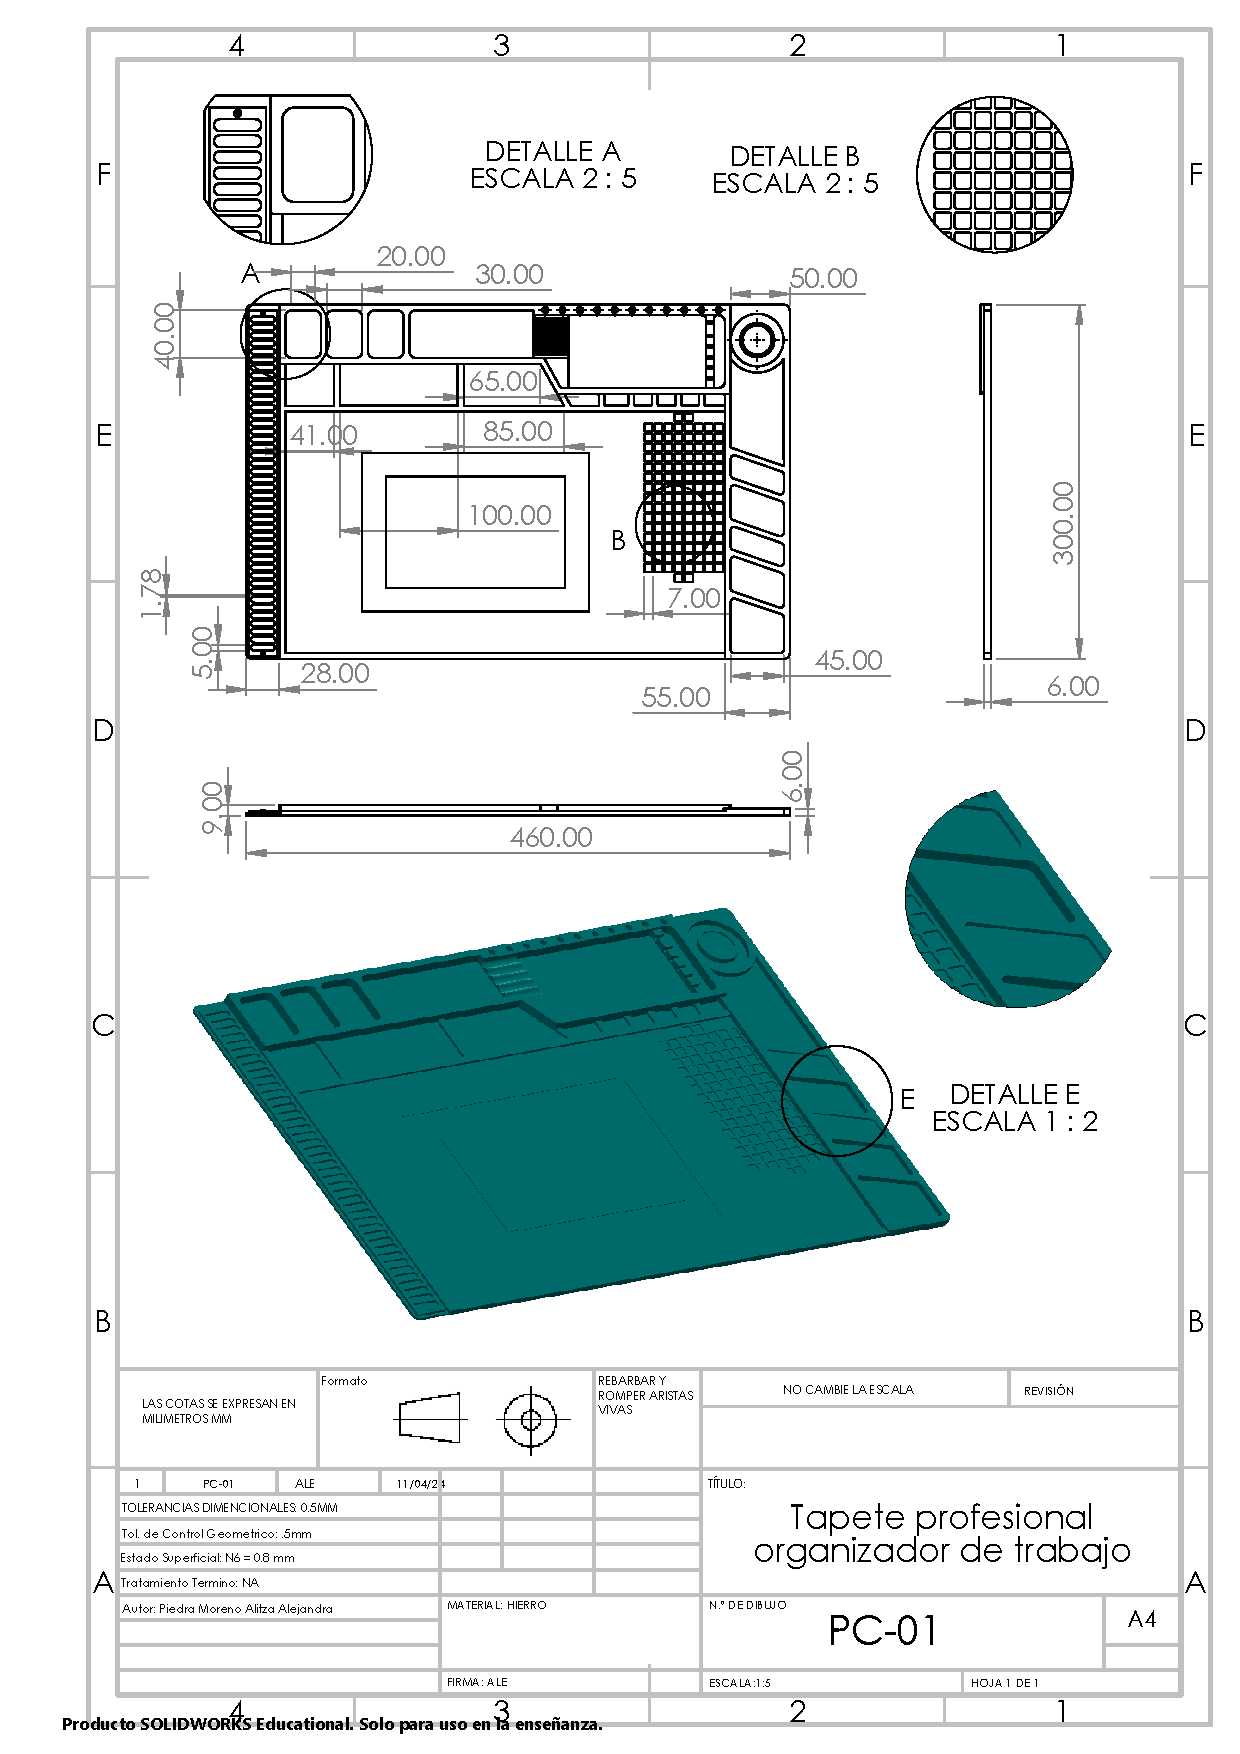
\includegraphics[trim = {7mm 1mm 1mm 1mm},clip,scale=0.4]{22/Img/almohadillaDibujo.pdf}
        \caption{Dibujo técnico de la almohadilla de trabajo}
        \label{fig:almohadillaD}
    \end{figure}
    
    Ahora que ya conocemos un poco más de la forma física de nuestro elemento, nos seguiremos a describirlo un poco más en sus propiedades, esto a razón de lo antes mencionado que es familiarizarnos primeramente con el método actual.
    
    Propiedad antiestática: Tiene áreas especiales para colocar procesadores, microchips, memorias, tarjetas de desarrollo o cualquier otro elemento de electrónica que pueda ser afectado por la estática. Incluso, te protege de las cargas estáticas almacenadas en los componentes en reposo.
    
    
    Propiedad magnética: Incorpora imanes distribuidos en lugares diferentes; perfectos para retener piezas metálicas, como tornillería, herramientas, puntas de desarmador, tarrajas y pinzas, entre otras. Además, pueden ser utilizados para magnetizar o desmagnetizar puntas de desarmadores.
    
    
    Espacios ideales para el trabajo:
    
    Mini ranuras: Perfectas para colocar las piezas de los equipos desarmados y llevar el control de su posición, gracias a que están numeradas.
    Mini cajones: Ayudan a identificar piezas pequeñas o tornillos indispensables para el reensamblaje de los equipos en reparación.
    Orificios: Útiles para que coloques tus desarmadores, aplicadores de flux o pastas en jeringa en una posición adecuada y puedas tomarlos rápidamente.
    Cajones multifunción: Estos compartimentos de diversos tamaños son apropiados para otros objetos misceláneos que utilices.
    Cajones con tapa: Adecuados para que almacenes y cuides los componentes más importantes.
    Cajones para herramientas: Tienen el espacio ideal para colocar pinzas, espátulas, punzones y más.
    Regleta: Es de 36 cm. Te servirá como referencia para trabajos en los que requieras medir.
    Espacio central: Es el área de trabajo perfecta donde puedes armar o desarmar los equipos.
    
    Material ideal para trabajar: Es flexible y tiene superficie antiderrapante. Está fabricado con silicona de textura suave al tacto que te da comodidad de uso y protege los equipos contra rayones y golpes. También puede ser usado para trabajos de soldadura, ya que soporta hasta 400 °C.
    
    
    
    \subsubsection{PC-02: Protoboard de 300 puntos}
    
    Un protoboard de 300 puntos es una placa de pruebas electrónica que se utiliza para prototipar circuitos electrónicos de manera temporal. Está diseñada con un patrón de agujeros y conexiones internas que permiten insertar y conectar componentes electrónicos de forma rápida y sin necesidad de soldadura. El “300 puntos” se refiere a la cantidad de puntos de conexión disponibles en la placa, lo que determina cuántos componentes y conexiones pueden alojarse en ella. Estos protoboards son herramientas muy útiles para diseñadores y estudiantes de electrónica, ya que les permiten experimentar y probar circuitos antes de realizar una implementación permanente.
    
    En la figura \ref{fig:proto} se muestra el diseño un tanto detallado de este elemento, como podemos ver tiene una dimensión de 55 x 82 mm, estas medidas son fundamentales a la hora de realizar nuestra distribución por lo cual necesario tenerlo en cuenta además que al tener presente que es de 300 puntos podemos destinar la posición de cada una de nuestras piezas así como optimizar nuestro ensamble.
    
    \begin{figure}[H]
        \centering
        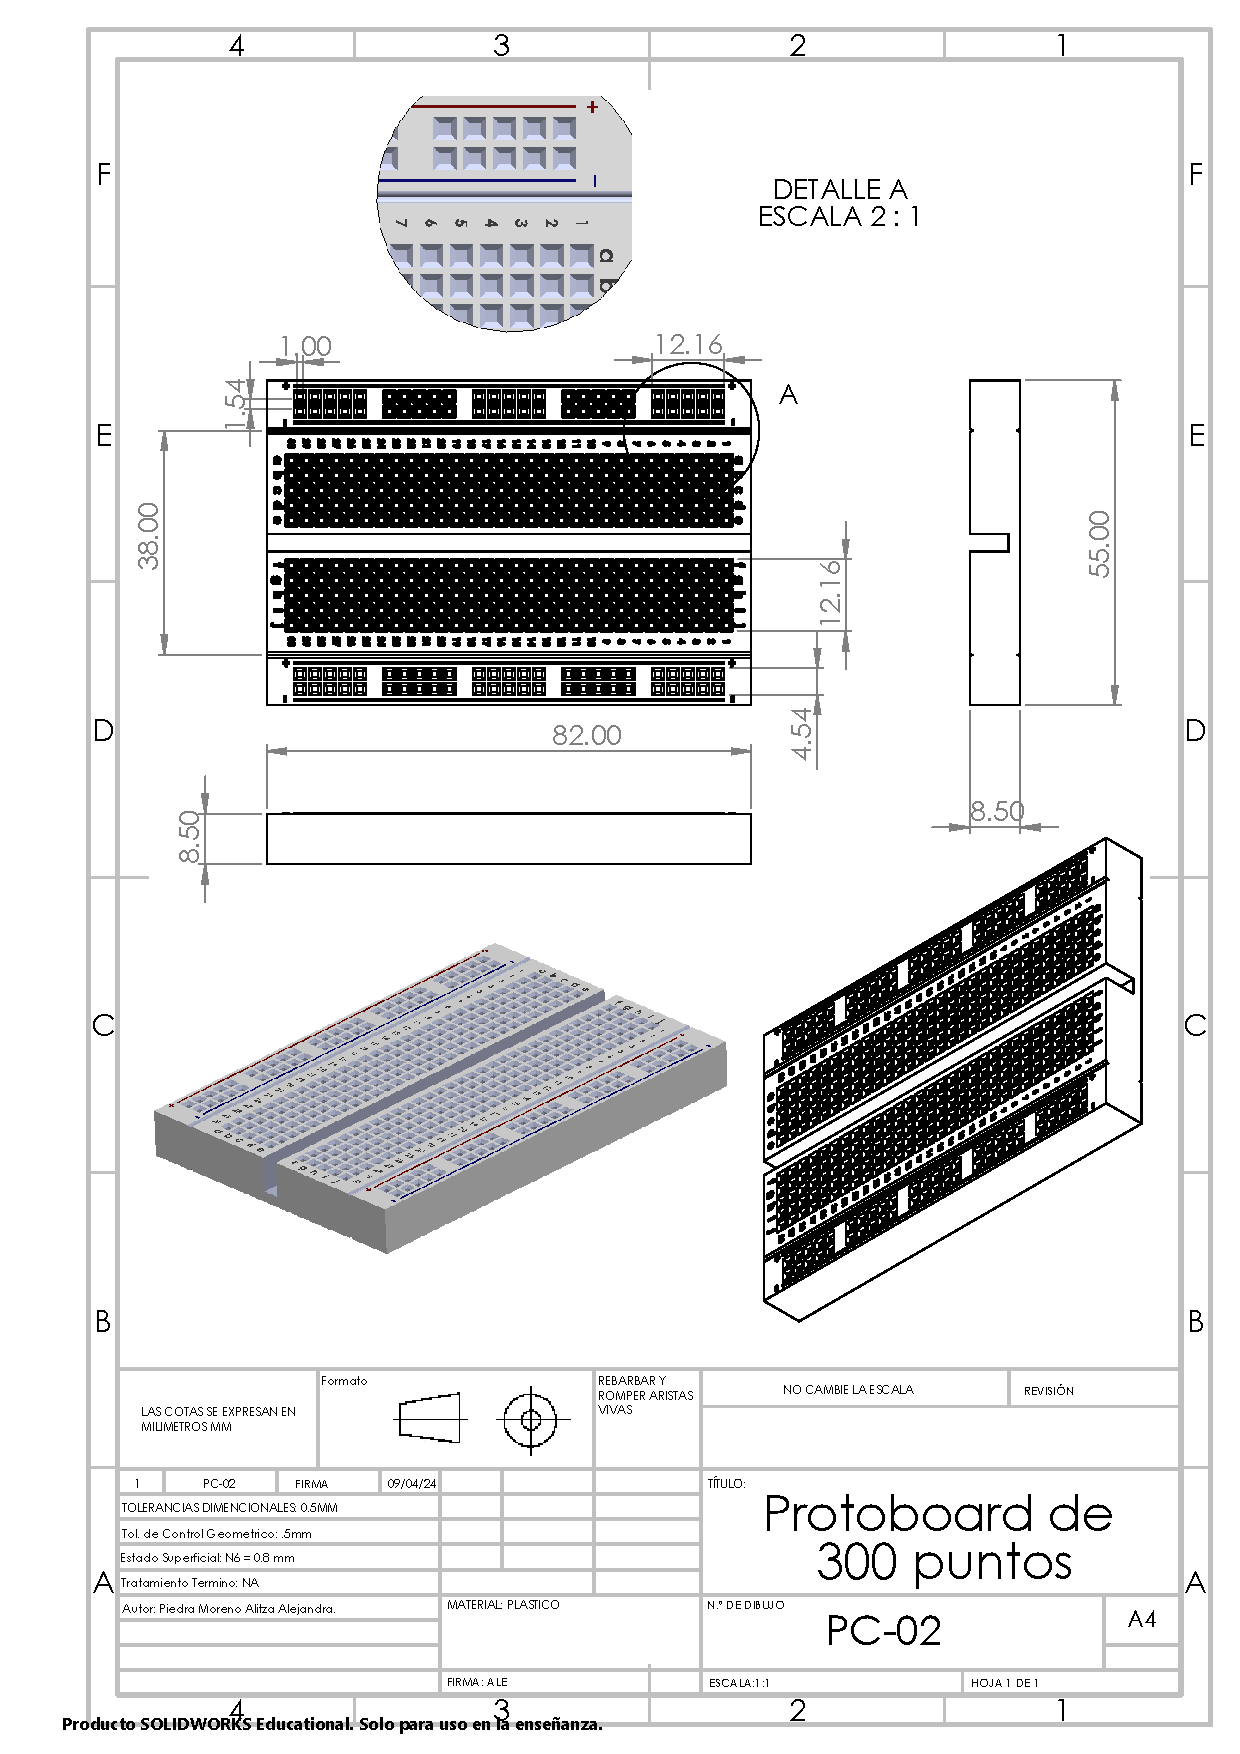
\includegraphics[trim = {7mm 1mm 1mm 1mm},clip,scale=0.4]{22/Img/protoDibujo.pdf}
        \caption{Dibujo técnico del protoboard de 300 puntos}
        \label{fig:proto}
    \end{figure}
    
    \subsubsection{PC-03: Pantalla de cristal líquido (LCD) 16X2}
    
    Una pantalla de cristal líquido (LCD) 16x2 es un tipo común de pantalla de visualización utilizada en una variedad de dispositivos electrónicos, como relojes, calculadoras, equipos de prueba, sistemas de control, y muchos otros dispositivos electrónicos. La designación “16x2” se refiere a la cantidad de caracteres que puede mostrar la pantalla en cada línea y el número de líneas, respectivamente, el 16, indica que la pantalla tiene 16 caracteres en cada línea horizontal. Esto significa que puede mostrar hasta 16 caracteres en una fila antes de pasar a la siguiente línea, mientras que el 2 indica que la pantalla tiene 2 líneas verticales de caracteres. Por lo tanto, puede mostrar dos líneas de texto o caracteres simultáneamente.
    \begin{figure}[H]
        \centering
        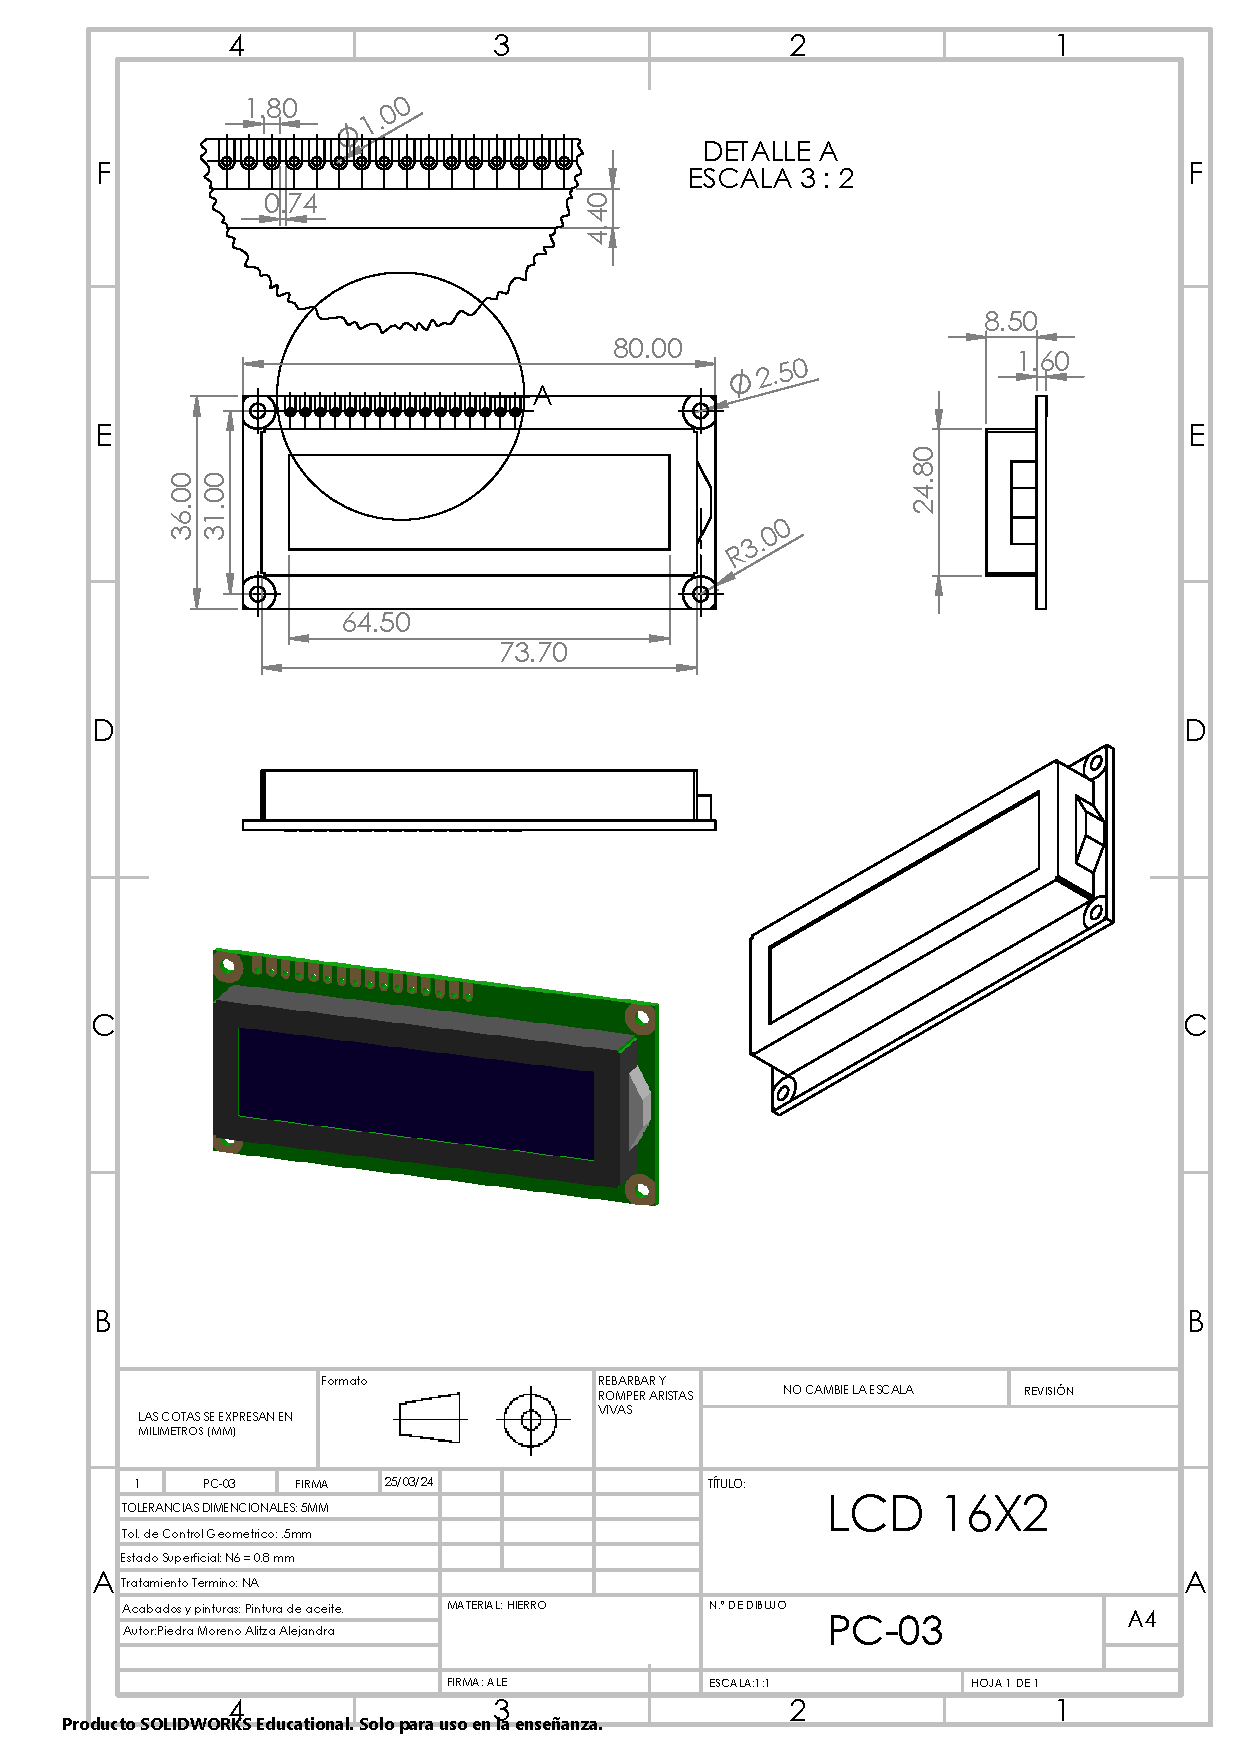
\includegraphics[trim = {7mm 1mm 1mm 1mm},clip,scale=0.4]{22/Img/lcdDibujo.PDF}
        \caption{Dibujo técnico de una LCD 16X2}
        \label{fig:lcd}
    \end{figure}
    
    Las pantallas LCD 16x2 generalmente funcionan con un controlador que facilita la comunicación con un microcontrolador o un dispositivo de procesamiento similar. Estas pantallas están compuestas por un conjunto de segmentos de cristal líquido que se activan eléctricamente para mostrar caracteres alfanuméricos, símbolos y otros tipos de información visual. Las pantallas LCD son populares debido a su bajo consumo de energía y su capacidad para mostrar información de manera clara y legible en una variedad de condiciones de iluminación.
    
    
    En la figura \ref{fig:lcd} se muestra el dibujo técnico de esta pantalla LCD, donde nos muestra dimensiones importantes que se deben tener en cuenta en nuestro análisis. Como se observa, la placa base de la lcd tiene una dimensión de 80x36 mm, además que podemos observar que contiene 16 pines o patitas que son las que nos permite mandarle señales a nuestra pantalla y a través de la interfaz esta tarea se nos facilita muchísimo más.
    
    
    
    \subsubsection{PC-04: Módulo I2C Interfaz LCD 16x2 }
    
    El módulo I2C Interfaz LCD 16x2 es un dispositivo que combina una pantalla LCD alfanumérica de 16 caracteres por 2 líneas con un controlador integrado y una interfaz de comunicación I2C. Este tipo de módulos se utilizan comúnmente en proyectos de electrónica y sistemas embebidos para proporcionar una interfaz de usuario visual.
    
    El funcionamiento del módulo I2C Interfaz LCD 16x2 es relativamente simple:
    
    Conexión física: El módulo se conecta a un microcontrolador u otro dispositivo maestro a través de dos cables: uno para la línea de datos (SDA) y otro para la línea de reloj (SCL) del bus I2C. Estas conexiones permiten que el microcontrolador envíe comandos y datos al módulo LCD.
    
    Inicialización: Antes de poder utilizar la pantalla LCD, es necesario inicializarla. Esto implica configurar el controlador del LCD para que se comunique correctamente con el microcontrolador y establecer parámetros como el contraste, el brillo y la posición del cursor.
    
    Envío de datos: Una vez inicializado, el microcontrolador puede enviar comandos y datos al módulo LCD a través del bus I2C. Estos datos pueden incluir caracteres individuales para mostrar en la pantalla, comandos de control para configurar el comportamiento del LCD (como borrar la pantalla, mover el cursor, etc.), o incluso mensajes completos que deben mostrarse en la pantalla.
    
    Actualización de la pantalla: El controlador del módulo LCD se encarga de traducir los comandos y datos recibidos del microcontrolador en acciones específicas en la pantalla. Esto puede incluir la activación y desactivación de píxeles individuales para mostrar caracteres, la actualización de la posición del cursor en la pantalla, o cualquier otra operación necesaria para reflejar los datos enviados por el microcontrolador en la pantalla LCD.
    
    En la figura \ref{fig:modulo} se muestran las medidas y detalles importantes que se deben conocer de este módulo de LCD
    \begin{figure}[H]
        \centering
        \includegraphics[trim = {7mm 1mm 1mm 1mm},clip,scale=0.4]{22/Img/móduloI2CInterfazDibujo.pdf}
        \caption{Dibujo técnico: Módulo I2C Interfaz LCD 16x2}
        \label{fig:modulo}
    \end{figure}
    
    
    \subsubsection{PC-05: ESP32-C6-WROOM-1 }
    El ESP-WROOM-32 es un potente módulo que integra WiFi y Bluetooth, ideal para desarrollar productos de IoT.  La integración de Bluetooth, Bluetooth LE y WiFi permite una amplia gama de aplicaciones, el uso de WiFi permite una comunicación de mediano alcance y conectarse a una red LAN y a través de un Modem Router conexión a Internet, mientras que el Bluetooth nos permite conectarse directamente a otro dispositivo como un celular.
    
    \begin{figure}[H]
        \centering
        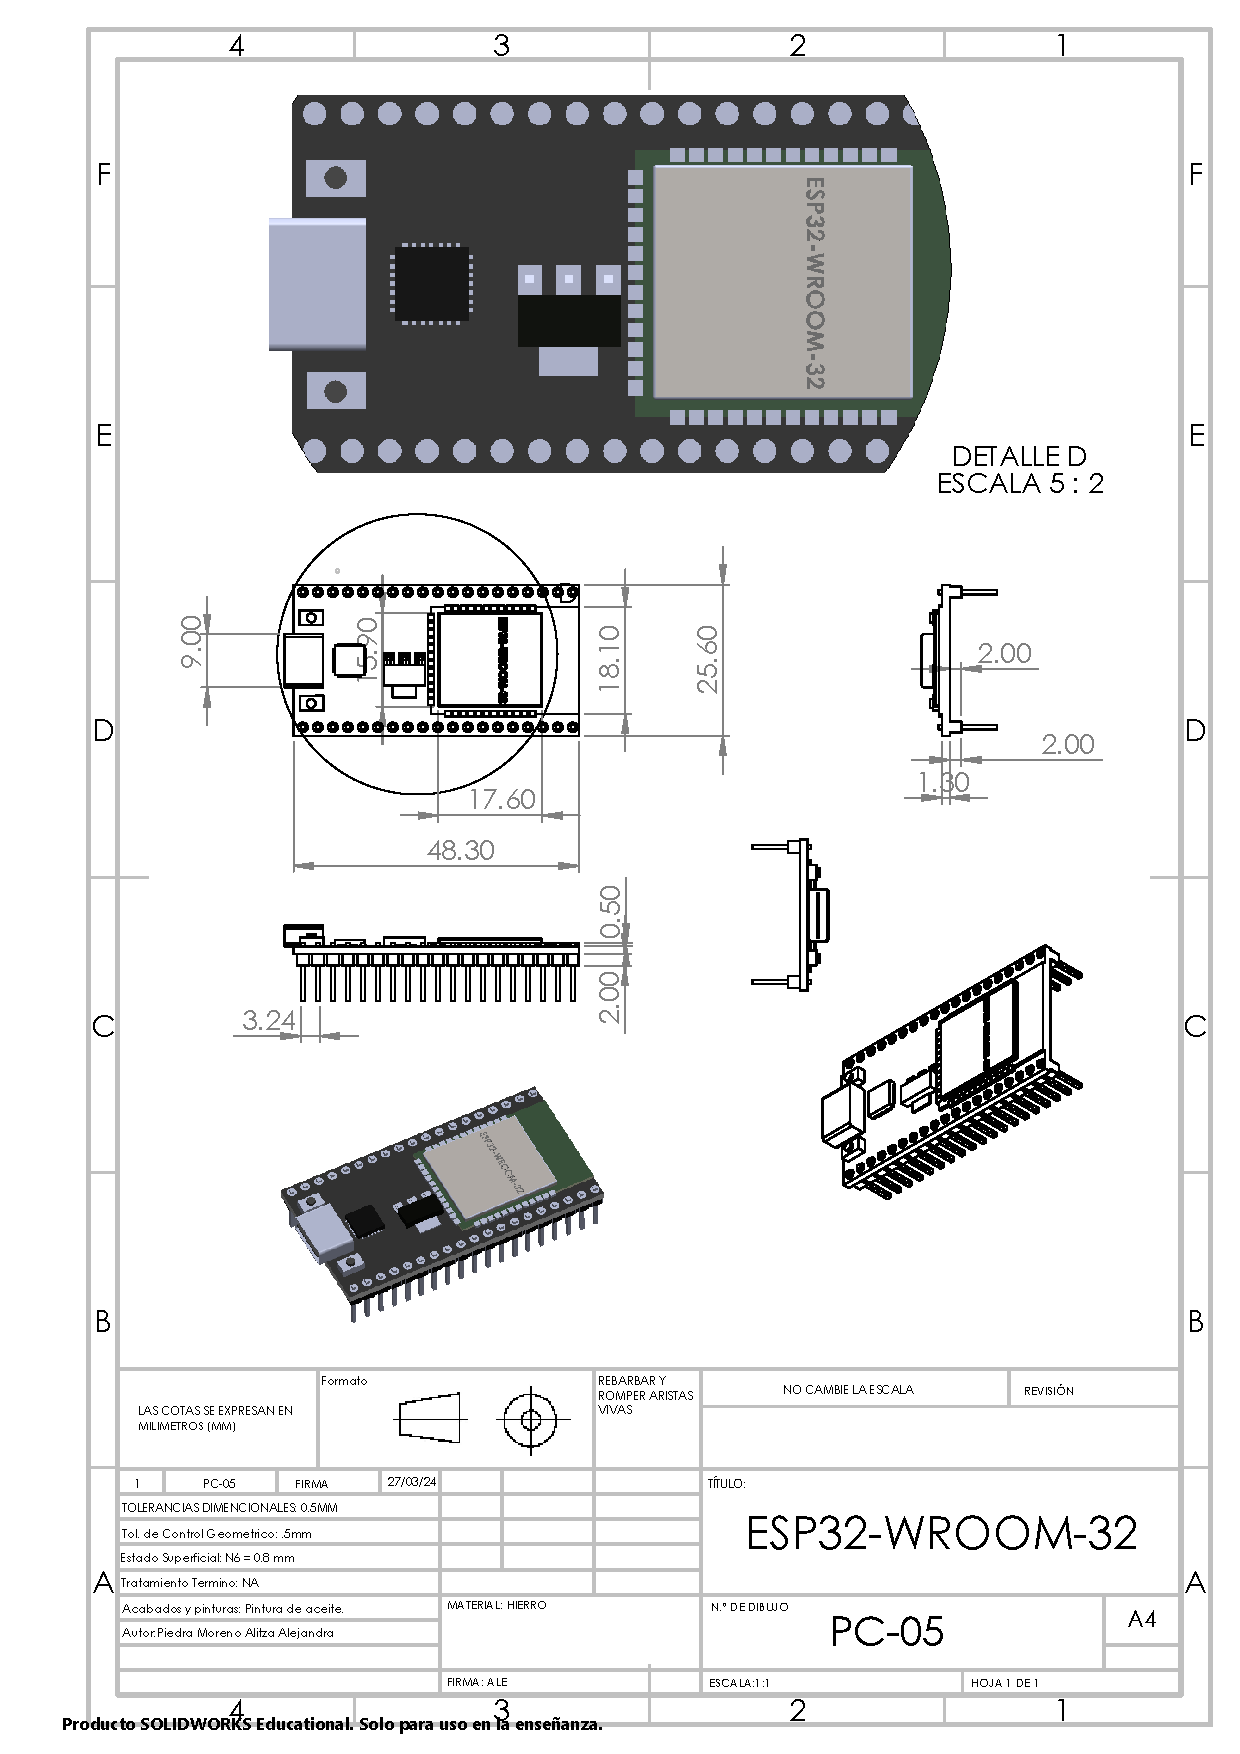
\includegraphics[trim = {7mm 1mm 1mm 1mm},clip,scale=0.4]{22/Img/esp32Dibujo.pdf}
        \caption{Dibujo técnico: ESP32-C6-WROOM-1}
        \label{fig:esp}
    \end{figure}
    
    La corriente de reposo del chip ESP32 es inferior a 5 uA, por lo que es adecuado para aplicaciones de electrónica portátiles con batería. En el núcleo de este módulo está el SoC ESP32-D0WDQ6. El chip integrado está diseñado para ser escalable y adaptado.
    
    Hay dos núcleos de CPU que se pueden controlar individualmente, y la frecuencia del reloj es ajustable de 80 MHz a 240 MHz. El usuario también puede apagar la CPU y utilizar el coprocesador de baja potencia para supervisar constantemente los periféricos para detectar cambios de estado. ESP32 integra un amplio conjunto de periféricos como sensores táctiles capacitivos, sensores Hall, amplificadores de bajo nivel de ruido, interfaz para SD, Ethernet, SPI, UART, I2S e I2C. Para flasher el chip es necesario utilizar un módulo conversor USB a serial TTL como el Módulo CP2102.
    El módulo ESP-WROOM-32 trabaja a 3.3 V en alimentación y GPIO por lo que NO se debe alimentar con 5 V. Se recomienda colocar un capacitor de 100uF en paralelo con la fuente de alimentación para filtrar los picos de corriente. Los pines de entradas/salidas (GPIO) trabajan a 3.3 V por lo que para la conexión a sistemas de 5 V es necesario utilizar conversores de nivel como: Conversor de nivel 3.3-5 V 4CH o Conversor de nivel bidireccional 8CH - TXS0108E.
    
    
    La plataforma ESP32 permite el desarrollo de aplicaciones en diferentes lenguajes de programación, frameworks, librerías y recursos diversos. Los más comunes a elegir son: Arduino(en lenguaje C++), Esp-idf(Espressif IoT Development Framework) desarrollado por el fabricante del chip, Simba Embedded Programming Platform(en lenguaje Python), RTOS's (como Zephyr Project, Mongoose OS, NuttX RTOS), MicroPython, LUA, Javascript (Espruino, Duktape, Mongoose JS), Basic. Al trabajar dentro del entorno Arduino podremos utilizar un lenguaje de programación conocido y hacer uso de un IDE sencillo de utilizar. Ademas de hacer uso de toda la información sobre proyectos y librerías disponibles en internet. La comunidad de usuarios de Arduino es muy activa y da soporte a plataformas como el ESP32 y ESP8266. Dentro de las principales placas de desarrollo o módulos basados en el ESP32 tenemos: ESP32-WROOM-32, NodeMCU-32 ESP32 y ESP32-CAM y de la familia ESP8266 tenemos: ESP-01, ESP-12E, Wemos D1 mini y NodeMCU v2.\cite{naylamp}
    
    
    
    \subsubsection{PC-06: Potenciómetro lineal 1k preciso }
    
    Un potenciómetro es un dispositivo conformado por 2 resistencias en serie, las cuales poseen valores que pueden ser modificados por el usuario. 
    
    En la figura \ref{fig:potenciometro} encontramos el dibujo técnico del potenciómetro que se usa en la operación con sus respectivas medidas y cotas.
    
    \begin{figure}[H]
        \centering
        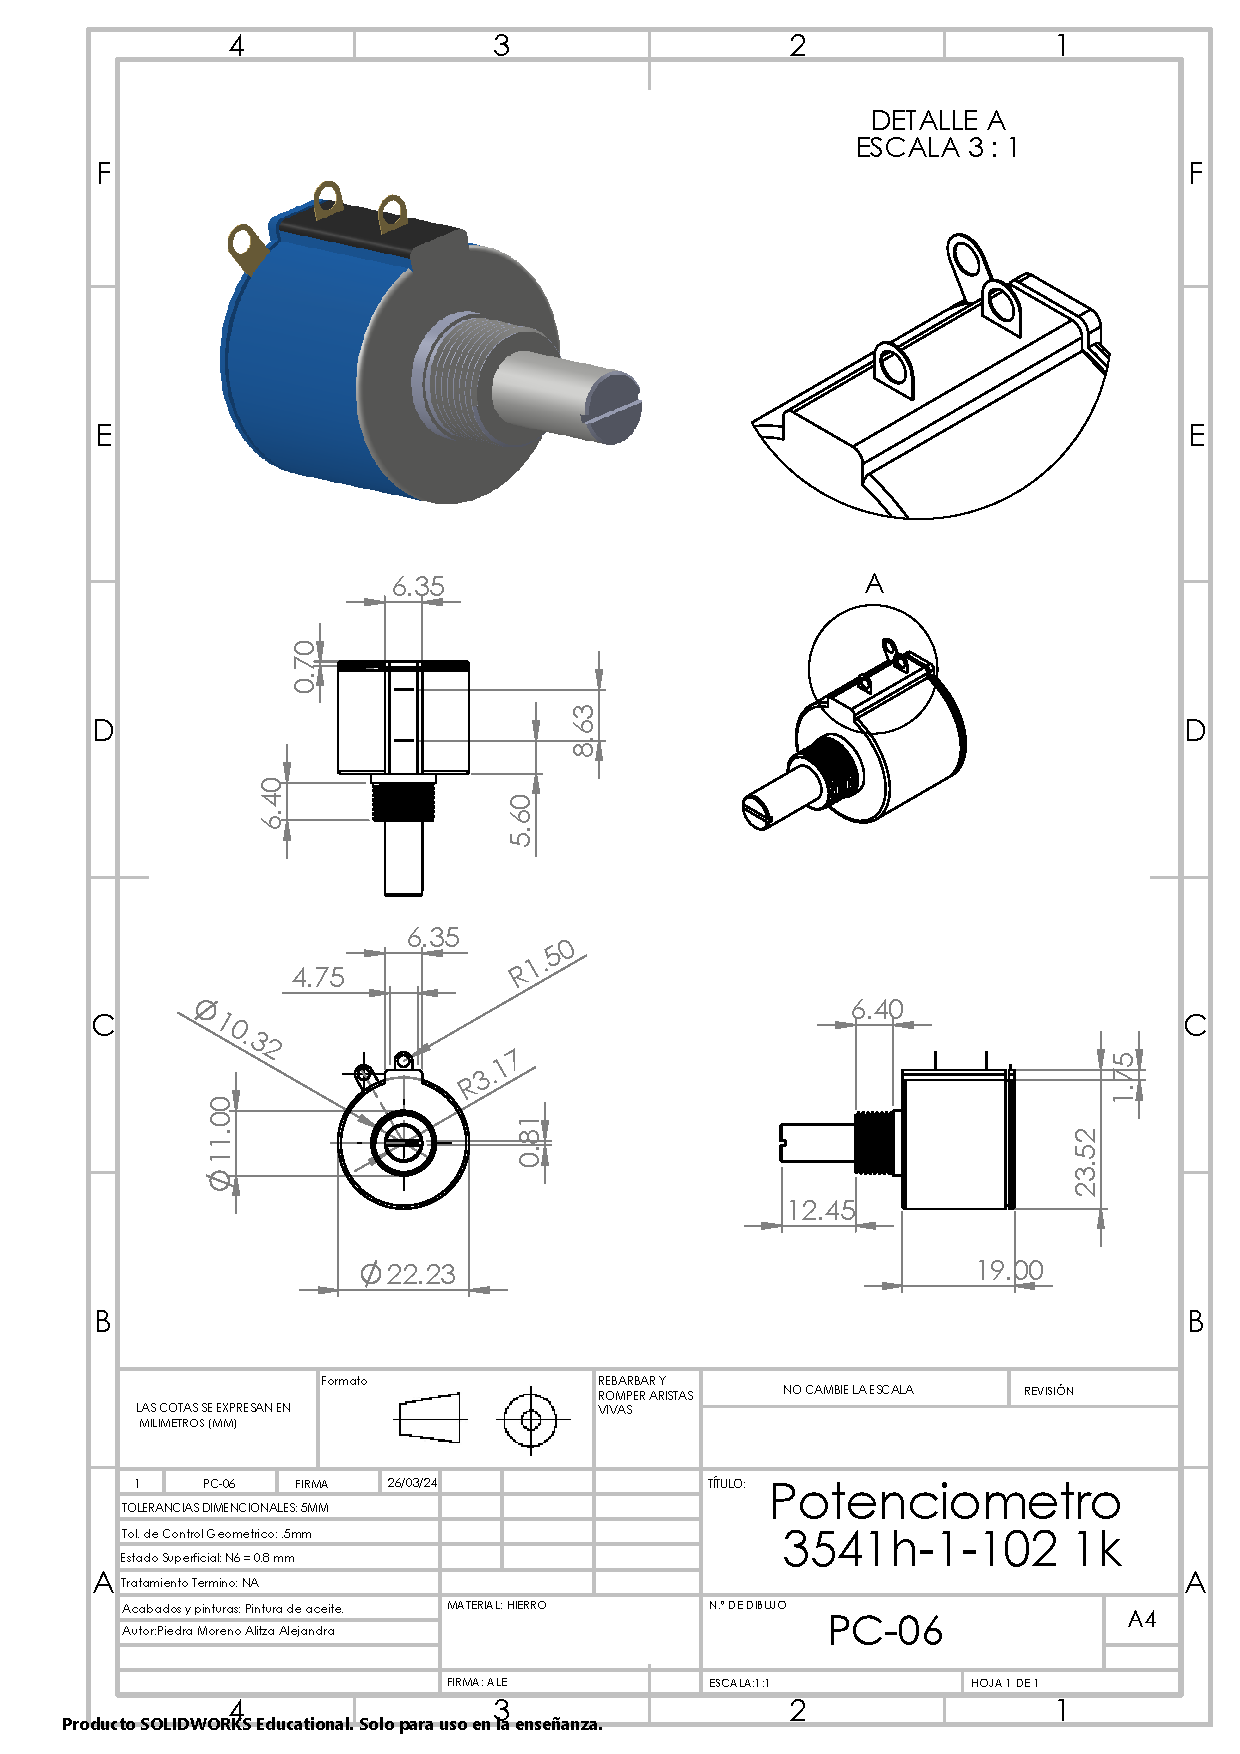
\includegraphics[trim = {7mm 1mm 1mm 1mm},clip,scale=0.4]{22/Img/potenciometroDibujo.PDF}
        \caption{Dibujo técnico: Potenciómetro lineal 1k preciso}
        \label{fig:potenciometro}
    \end{figure}
    
    
    \subsubsection{PC-07: Resistencia de 330 ohms 1/4 W }
    La resistencia es una medida de la oposición al flujo de corriente en un circuito eléctrico. La resistencia se mide en ohmios, que se simbolizan con la letra griega omega ($\Omega$). Se denominaron ohmios en honor a Georg Simon Ohm (1784-1854), un físico alemán que estudió la relación entre voltaje, corriente y resistencia. Se le atribuye la formulación de la ley de Ohm.
    
    
    
    
    
    Todos los materiales resisten en cierta medida el flujo de corriente. Se incluyen en una de dos amplias categorías:
    
    Conductores: materiales que ofrecen muy poca resistencia, donde los electrones pueden moverse fácilmente. Ejemplos: plata, cobre, oro y aluminio.
    Aislantes: materiales que presentan alta resistencia y restringen el flujo de electrones. Ejemplos: goma, papel, vidrio, madera y plástico.
    Normalmente, se toman las mediciones de resistencia para indicar las características de un componente o un circuito.
    \begin{figure}[H]
        \centering
        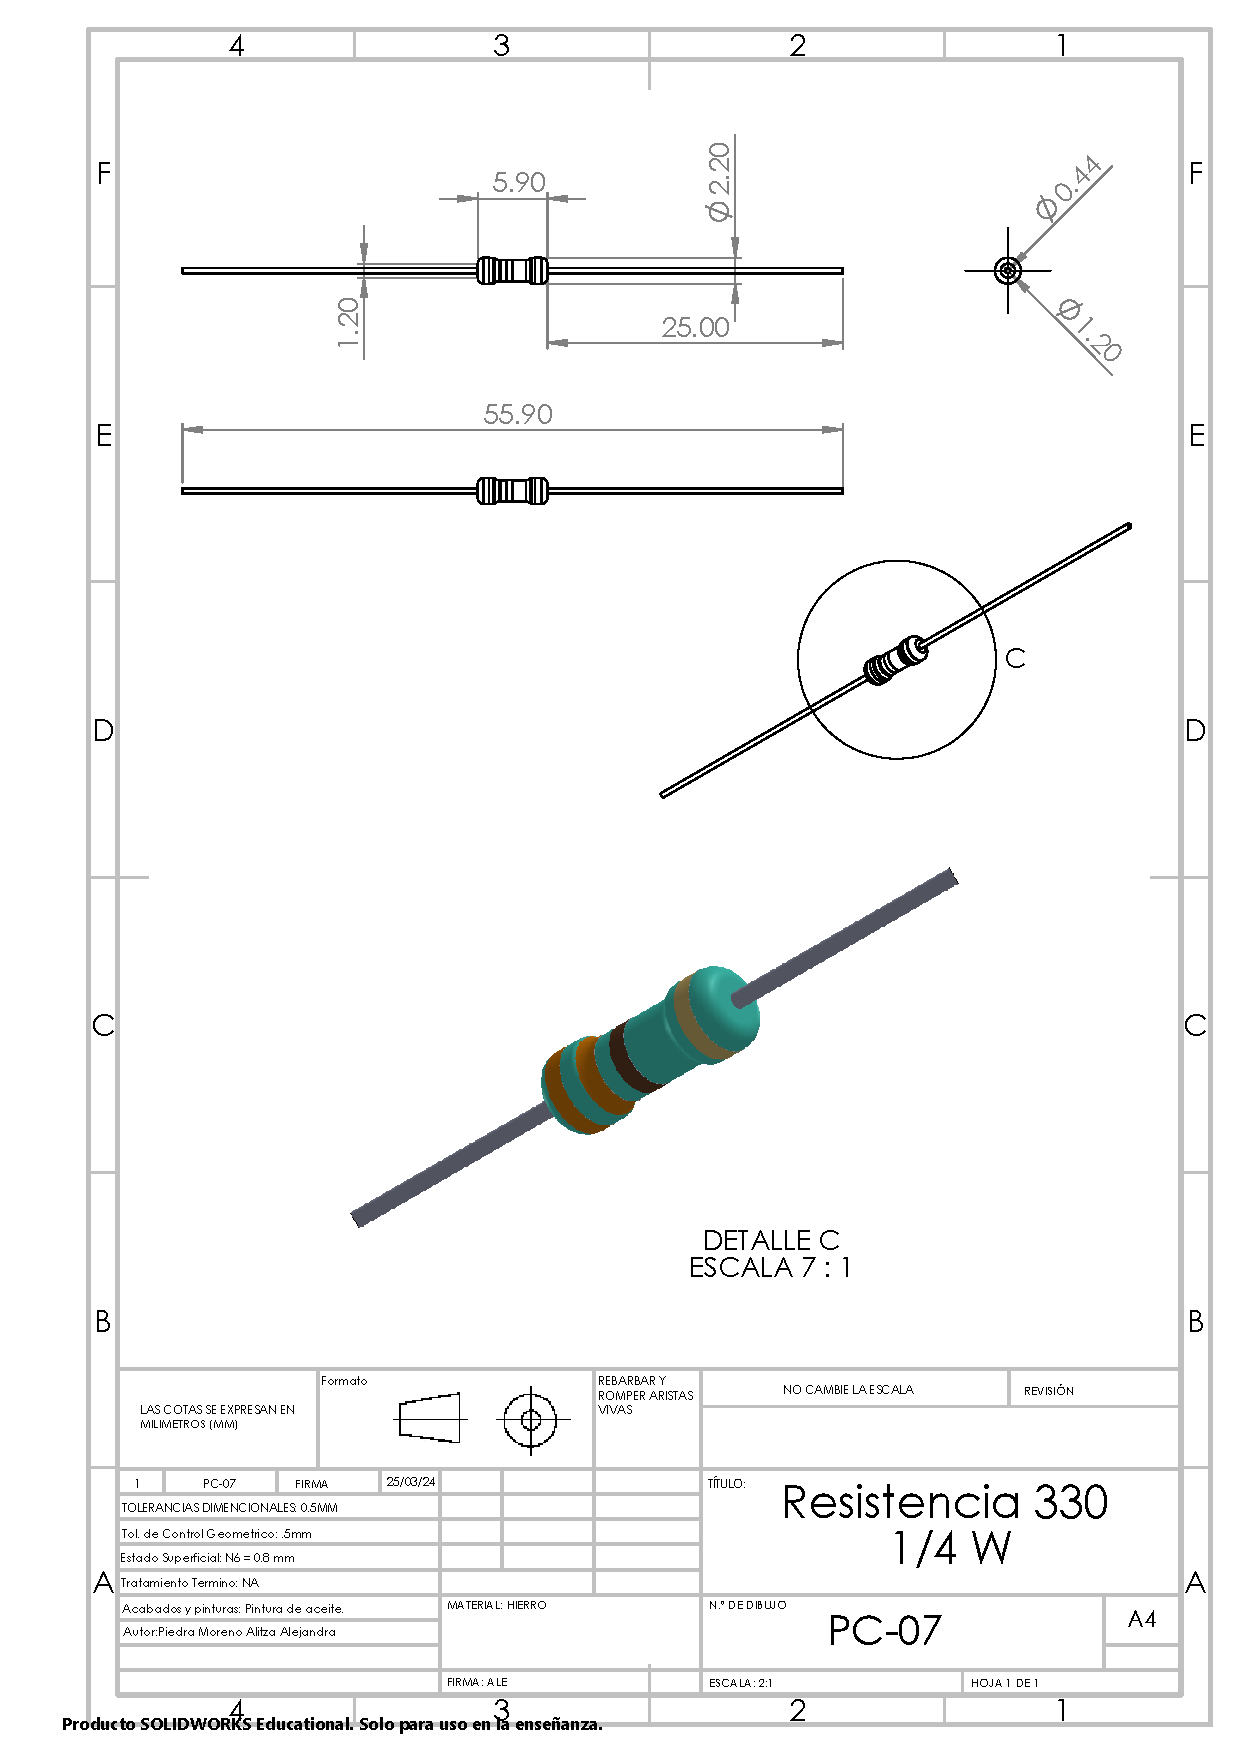
\includegraphics[trim = {7mm 1mm 1mm 1mm},clip,scale=0.4]{22/Img/resistenciaDibujo.PDF}
        \caption{Dibujo técnico: Resistencia de 330 ohms 1/4 W}
        \label{fig:resistencia}
    \end{figure}
    Cuanto mayor sea la resistencia, menor será el flujo de corriente. Si es anormalmente alta, una causa posible (entre muchas) podrían ser los conductores dañados por el fuego o la corrosión. Todos los conductores emiten cierto grado de calor, por lo que el sobrecalentamiento es un problema que a menudo se asocia con la resistencia.
    
    Cuanto menor sea la resistencia, mayor será el flujo de corriente. Causas posibles: aisladores dañados por la humedad o un sobrecalentamiento.
    Muchos componentes, tales como los elementos de calefacción y las resistencias, tienen un valor de resistencia fijo. Estos valores se imprimen a menudo en las placas de identificación de los componentes o en los manuales de referencia.
    
    Cuando se indica una tolerancia, el valor de resistencia debe encontrarse dentro de la gama de la resistencia especificada. Cualquier cambio significativo en un valor de resistencia fijo generalmente indica un problema. \cite{Fluke}
    
    
     En la figura \ref{fig:resistencia} podemos observar el dibujo técnico de nuestras residencias de 330 ohms, incluyendo sus vistas y cotas.
     \begin{figure}[H]
        \centering
        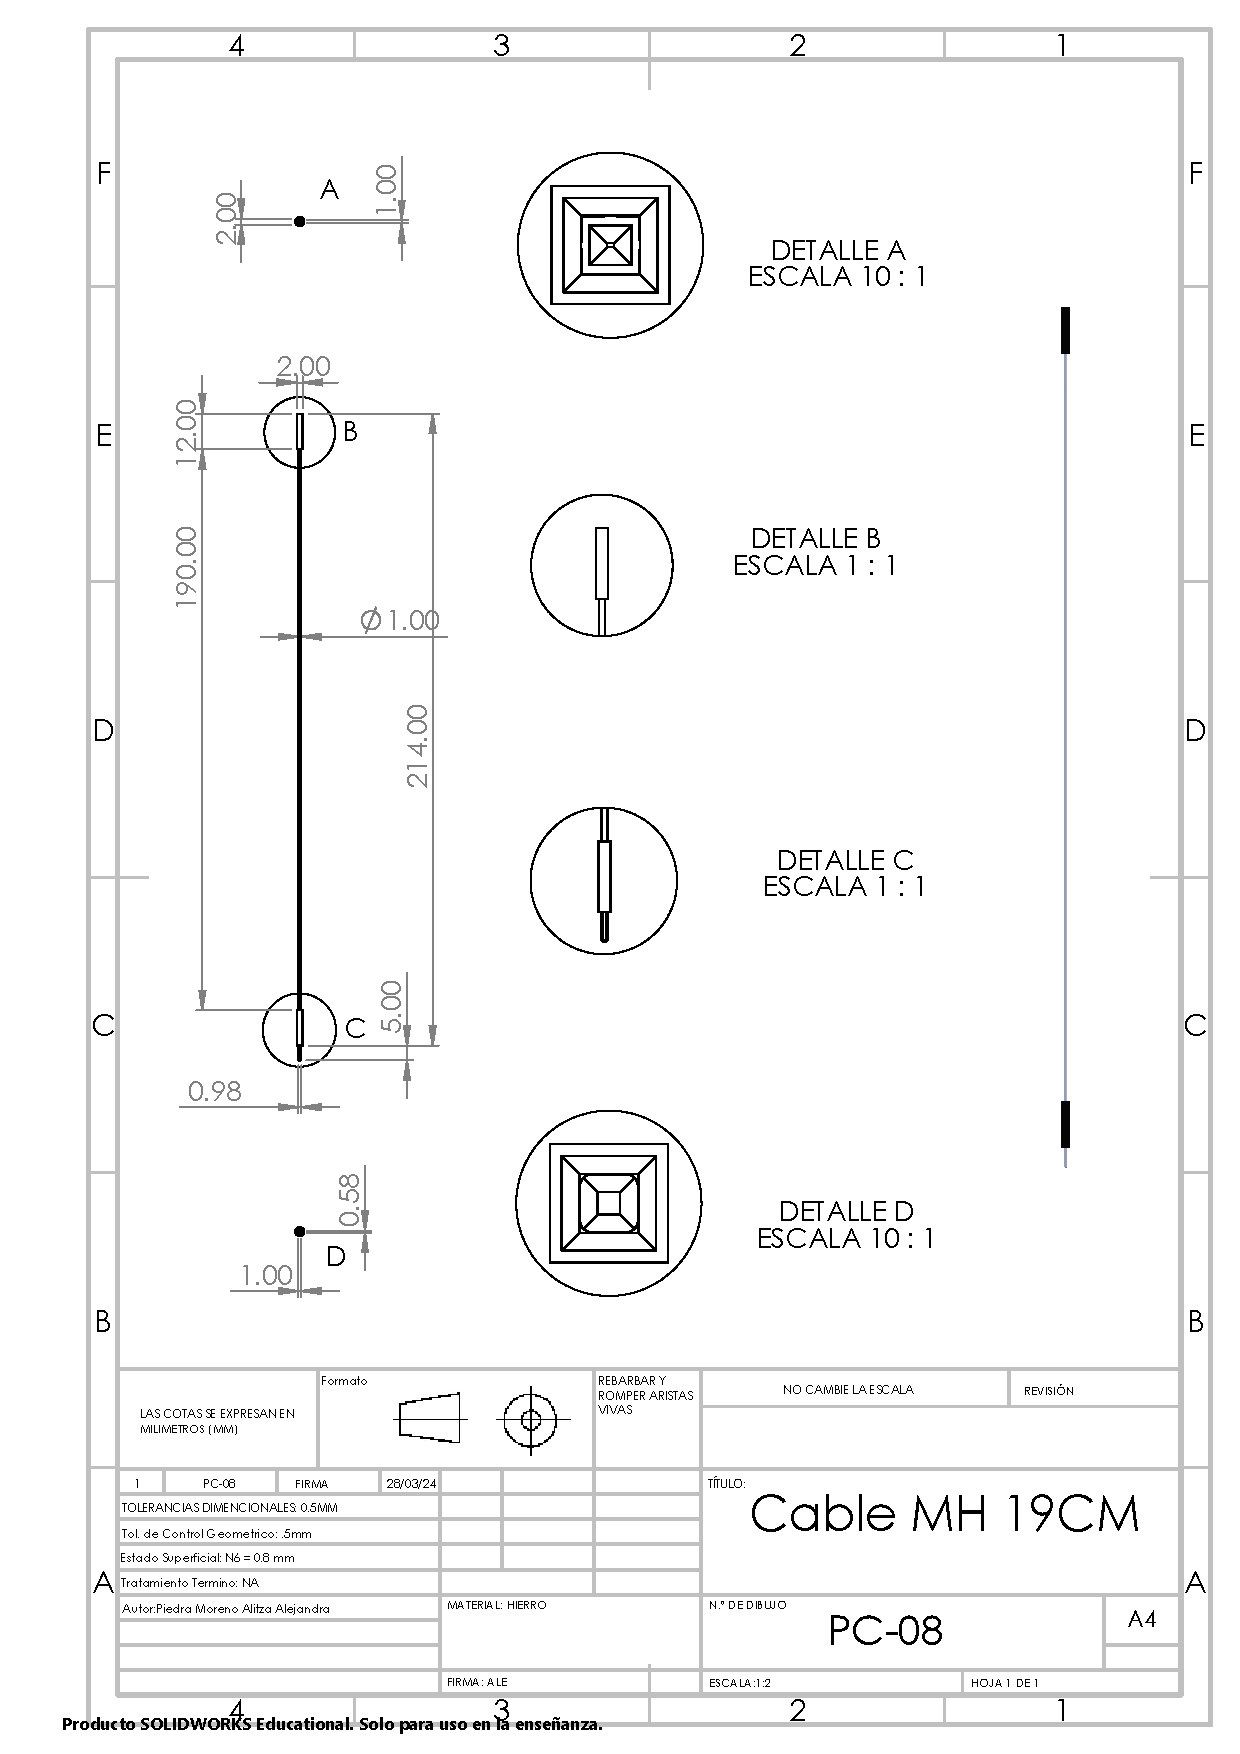
\includegraphics[trim = {7mm 1mm 1mm 1mm},clip,scale=0.4]{22/Img/cableMHDibujo.PDF}
        \caption{Dibujo técnico: Cable MH}
        \label{fig:Cable MH}
    \end{figure}
    
    \subsubsection{PC-08: Cables DuPont }
    
    Conector DuPont es un término vernáculo que se refiere a varios tipos diferentes de conectores de paso de 0,1 pulgadas. Cuentan con carcasas de plástico negro que retienen contactos con dedos integrados en el cuerpo de la carcasa. Todos son muy similares en apariencia, pero varían significativamente en calidad y precio.
    
    A menudo se les atribuyen otros nombres, como “Conector TYU” o “Conector JWT” (deje un comentario si conoce otro). Estos son acrónimos de algunos de los muchos fabricantes chinos, a veces moldeados físicamente en el producto. \cite{Mateo}
    
    Se utilizan principalmente como cables puente en protoboards y para interconectar tarjetas de desarrollo con sensores, módulos, actuadores, motores, etc. Suelen verse mucho en proyectos con Arduino o Raspberry Pi y son un material que se ha vuelto indispensable para estudiantes que trabajan con circuitos electrónicos. 
    
    Véase la figura \ref{fig:Cable MH} para observar las medidas de un cable DuPont macho-hembra de 10 cm y en la figura \ref{fig:Cable MM} para el cable mach-macho igualmente de 10 cm.
    
    
    
    \begin{figure}[H]
        \centering
        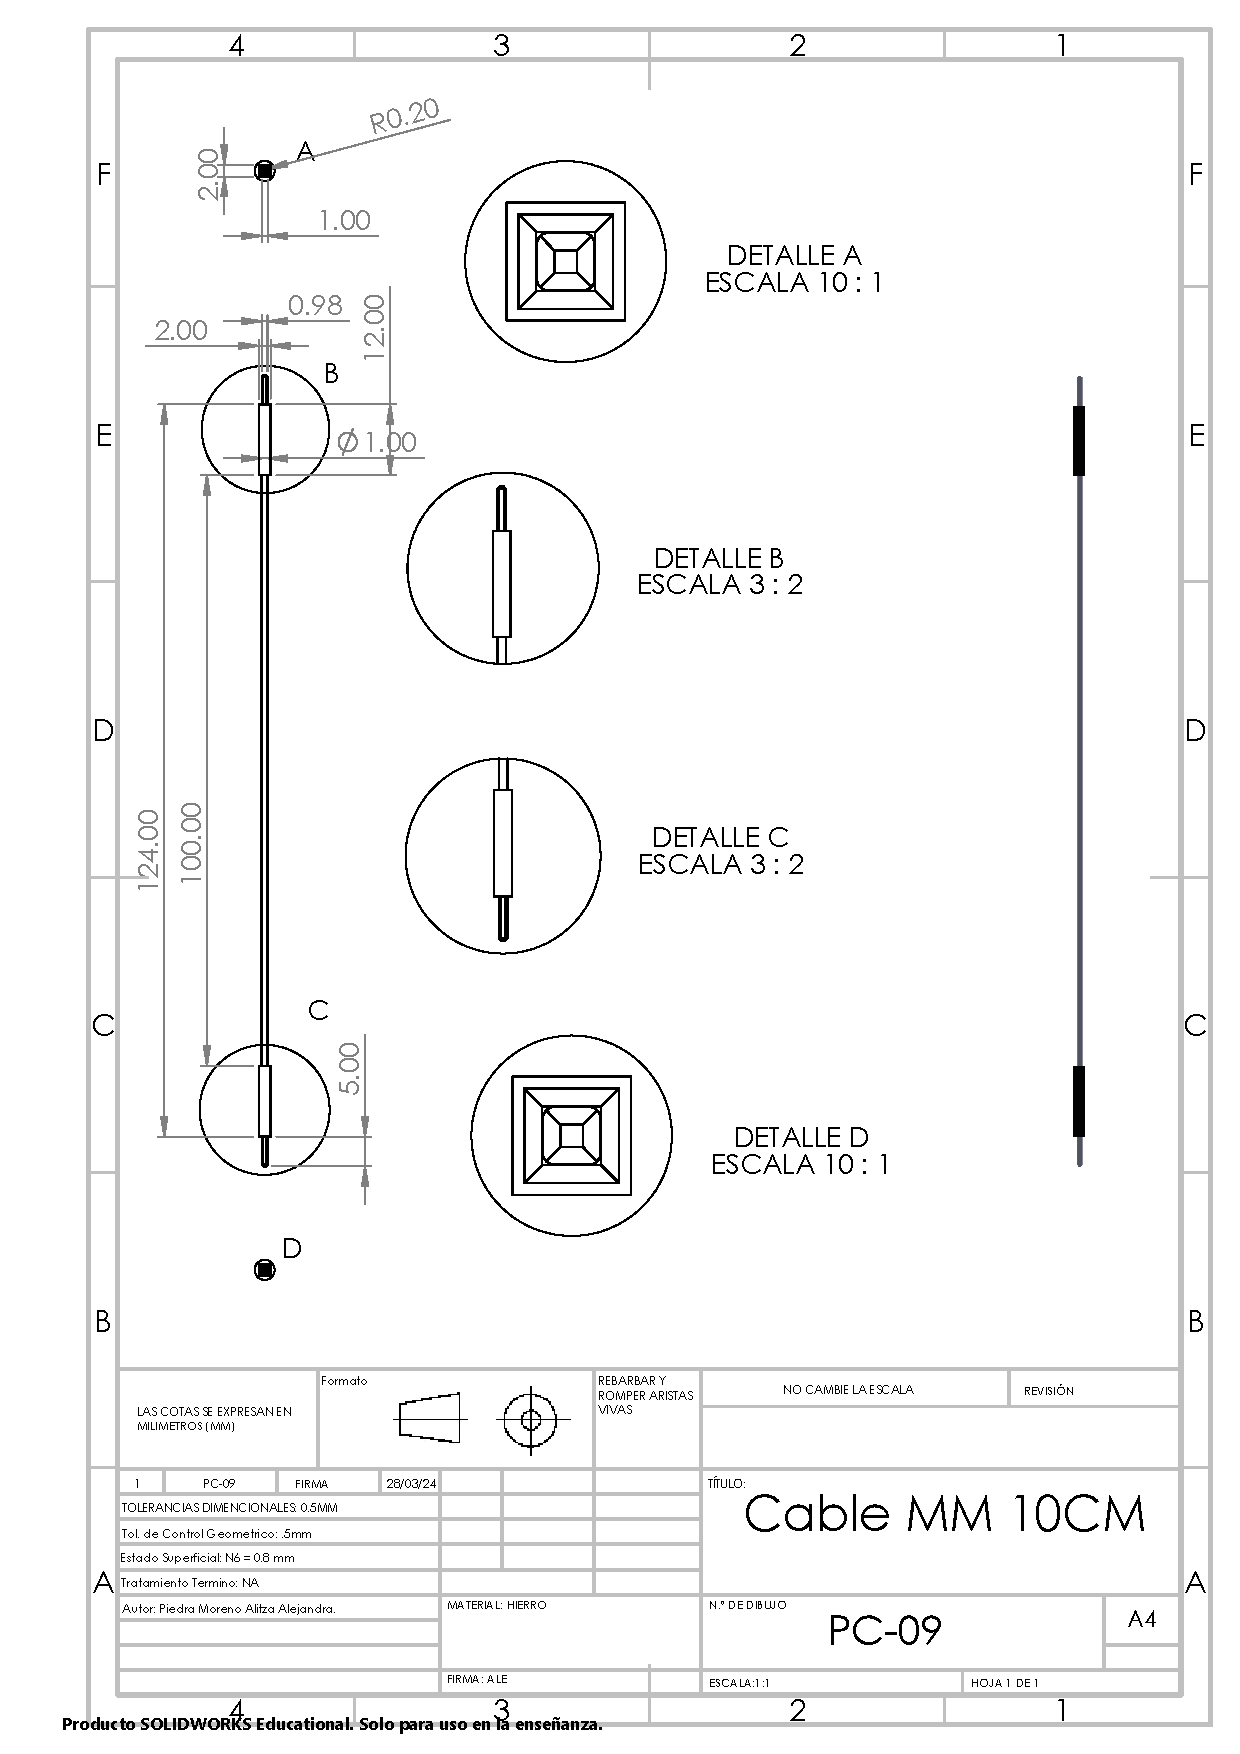
\includegraphics[trim = {7mm 1mm 1mm 1mm},clip,scale=0.4]{22/Img/cableMMDibujo.PDF}
        \caption{Dibujo técnico: Cable MM}
        \label{fig:Cable MM}
    \end{figure}
    
    \subsubsection{PC-10: Regulador Multicontacto Con 8 Salidas 3 USB Y 1 Tipo C }
    
    Las extensiones eléctricas y las barras multicontacto son útiles cuando un contacto no queda cerca del aparato que se desea conectar, o bien, no es suficiente para conectar más de dos aparatos al mismo tiempo.
    La descripción de la regleta que nosotros utilizamos es la siguiente:
    
    Regleta de alimentación con 8 salidas de CA y 4 barras de alimentación USB con protector contra sobretensiones con 8 tomas de CA y 4 puertos de carga USB (1 toma USB C). Cable de extensión de 1.2 m de alta resistencia (1625 W/13 A), protector contra sobretensiones (1700 julios) con protección contra sobrecargas que protege contra picos y fluctuaciones.
    
    Carga rápida e inteligente USB-C: 4 puertos USB 3.4 A en total, cada puerto USB A cuenta con una salida máxima de 2.4 A. El puerto de carga USB C cuenta con 3A MAX. Construido con tecnología inteligente, detecta los dispositivos de carga y ofrece una velocidad de carga óptima de forma automática, compatible con la mayoría de los dispositivos USB.
    
    NOTA: El puerto UCB-C no es compatible con ningún otro dispositivo que necesite
    salidas de protección contra sobretensiones de 8 AC con un voltaje de carga de 14 22 V: el circuito protector contra sobretensiones complementario de 3 niveles, compuesto por TVS (supresor de voltaje transitorio), con una capacidad mínima de absorción de energía de 2700 julios, podría proteger sus dispositivos mucho más de forma rápida y confiable que los circuitos de protección contra sobretensiones MOV de 1 nivel de otras marcas.
    
    Seguridad y certificado: certificación de seguridad ETL, con cable de extensión y otros componentes principales certificados por UL. El interruptor de protección contra sobrecorriente limita la corriente de trabajo de la regleta a una configuración determinada, por lo que no se calentará durante el uso. La carcasa de PC con protección ambiental y resistencia al fuego con retardante de llama a 1382 F hace que sea más duradera y tenga una vida útil más larga.
    
    Lo que obtiene: regleta, devolución en 30 días, nuestro servicio de atención al cliente confiable y sin preocupaciones de 24 meses le responderá en 24 horas.
    
    
    Para tener una noción del tamaño, véase la figura \ref{fig:multicontacto}, en donde se muestra el dibujo técnico de la pieza, y coloca las medidas correspondientes de estas, así como sus vistas.
    \begin{figure}[H]
        \centering
        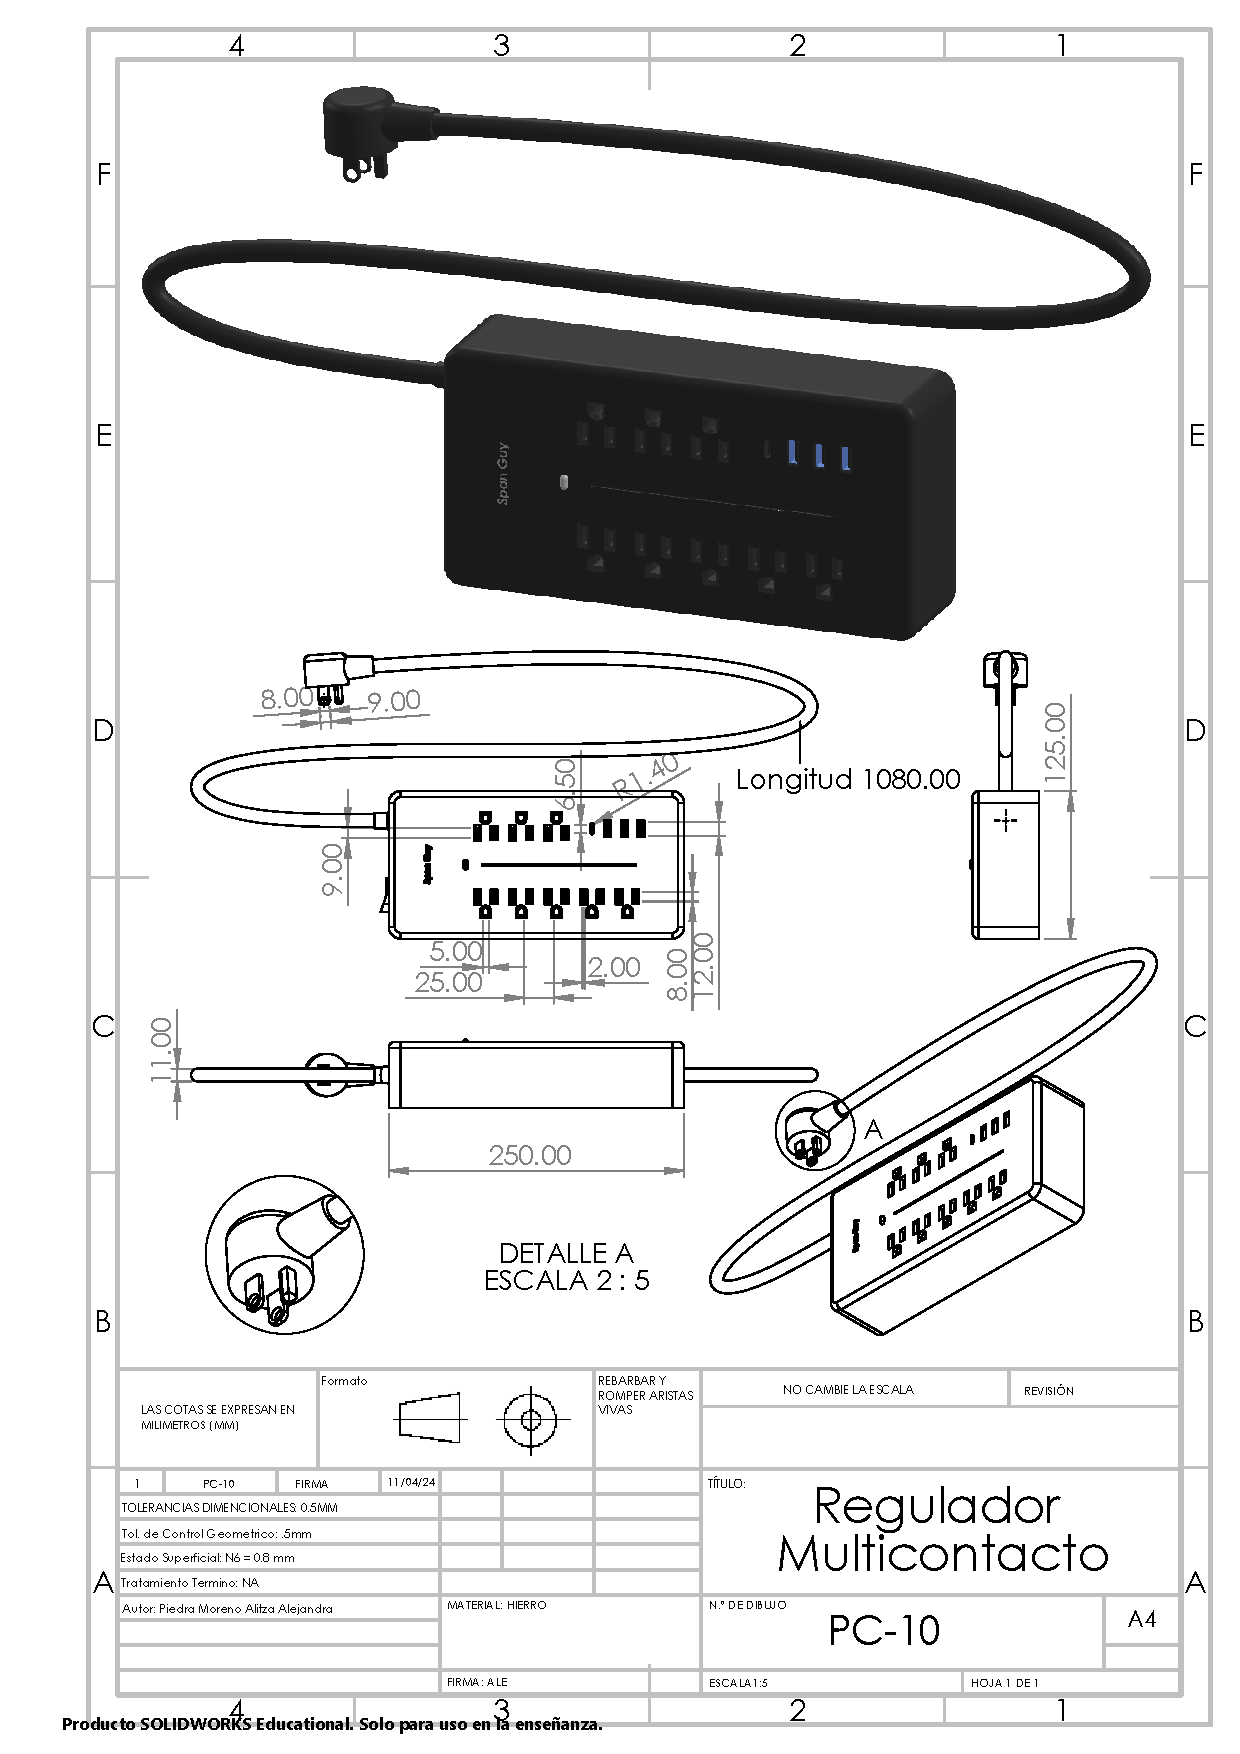
\includegraphics[trim = {7mm 1mm 1mm 1mm},clip,scale=0.4]{22/Img/multicontactoDibujo.pdf}
        \caption{Dibujo técnico: Cable MM}
        \label{fig:multicontacto}
    \end{figure}
    
    \subsubsection{PC-11: Cable Tipo C }
    Se trata de un conector de formato pequeño doble cara de 24 pines. Es conocido por facilitar la transferencia de datos y archivos de manera rápida entre diferentes dispositivos.
    
    La ventaja de este tipo de cable, es que su velocidad de transferencias es de hasta 10 GB/s. Asimismo, es capaz de proporcionar energía a través de la carga rápida, que es una tecnología adaptada a los móviles y dispositivos para alcanzar un mayor nivel de batería en menos tiempo.
    
    Para conocer más este cable véase la figura \ref{fig:cableC}, en donde podemos encontrar las medidas y vista de nuestra pieza a utilizar. 
    
    \begin{figure}[H]
        \centering
        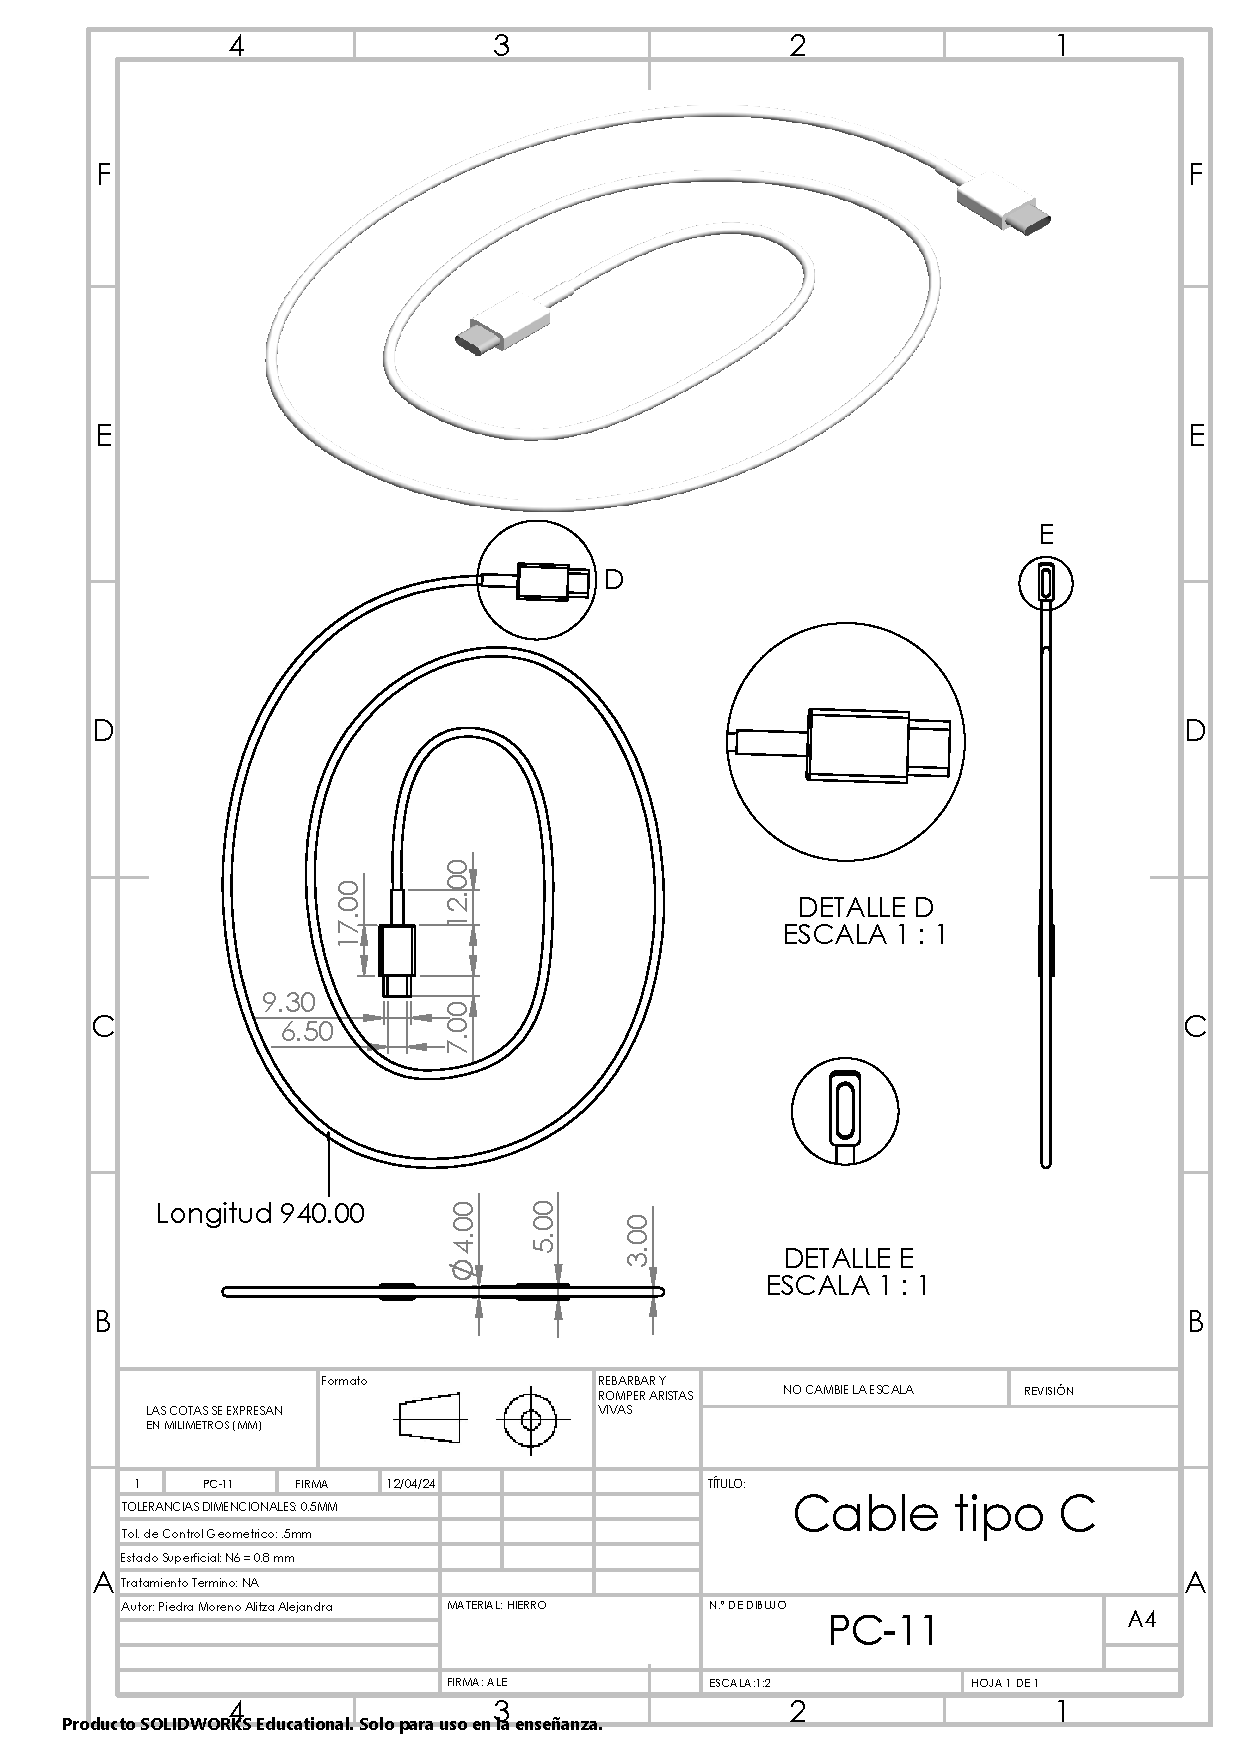
\includegraphics[trim = {7mm 1mm 1mm 1mm},clip,scale=0.4]{22/Img/cableCDibujo.PDF}
        \caption{Dibujo técnico: Cable MM}
        \label{fig:cableC}
    \end{figure}
    
    %https://www.acerstore.cl/news/usb-tipo-c-que-es-y-para-que-sirve/%
    \subsubsection{5's}
    
    Tener solo lo que se necesita en el momento que se necesita, ordenar todo de acuerdo a la frecuencia de uso, mantener todo limpio,  en óptimas condiciones de operación y todo lo anterior, convertirlo en una forma de vida. Este podría decirse que es una forma corta de resumir lo que implica las 5´s o en sí, su definición.
    
    La qué metodología de las 5´s ayuda a incrementar la eficiencia y seguridad en el lugar de trabajo al promover la organización y limpieza. Al eliminar el desorden y estandarizar procesos, se reducen costos y se aumenta la calidad del trabajo. Además, ayuda a  prevenir accidentes y fomentar la participación del personal en la mejora continua. 
    
    
    Por esto mismo, en el proyecto integrador se tiene como objetivo la aplicación  de esta metodología, incluyéndola principalmente en la distribución inicial del área del ensamblaje, ya que se debe incluir desde las cosas más simples.
    
    % 
    \subsubsection{Desarrollo del sistema de tiempos predeterminado}
    % 
    % 
    \subsubsection{Desarrollo del muestreo del trabajo}
    % 
    % 
    \subsubsection{Corrección por balanceo de procesos}
    % 
    % 
    \subsubsection{Datos estándares continuos y discretos}
    
    % 
    
    % 
    % 
    \subsection{Diseño de la forma más económica de realizar el trabajo}
    
    % 
    % 
    \subsection{Normalización de los métodos, materiales, herramientas e instalaciones}
    
    % 
    % 
    \subsection{Determinación del tiempo estándar para que una persona competente realice el trabajo con marcha normal}
    
    
    
    Como empresa es importante la mejora continua la cual concite en optimizar, proceso, herramientas e instalaciones, por ello mismo se debe llevar distintos métodos para el desarrollo de esta mejora, pero primero que nada uno como analista debe desglosar y familiarizarse con el método actual, ya que para un buen análisis debemos tener en cuenta todos los factores implicados en el trabajo y además es necesario para una comparativa del antes y él después esto para una mejor aceptación del nuevo método.
    
    Por ello mismo en la figura \ref{fig:Distribucion inicial}se muestra la distribución propuesta para la primera parte del análisis donde aún es con el método actual, lo cual es indispensable para notar los cambias y por ello mismo el operario debe asegurar que esta distribución se cumpla a la hora de realizar la operación.
        \begin{figure}[H] 
        \centering
        \includegraphics[trim = {1mm 1mm 1mm 1mm},clip,scale=0.3]{22/Img/ensamblaje.pdf}
        \caption{Distribución inicial}
        \label{fig:Distribucion inicial}
    \end{figure}
    
    Con esta propuesta de distribución podemos ahora si incursionar al lector a los procedimientos que el operario debe seguir para el desarrollo del ensamble del circuito electrónico, el cual es el método presente o el método propuesto a la mejora y se presenta en la siguiente lista:
    \begin{enumerate}
    
        \item Posiciona el protoboard en el área de ensamblaje.
    
        \item Coloca la ESP32 en el centro del protoboard colocando los pines NC en la columna 30 y en las filas B e I de forma que el pin 3V3 esté en el punto 15-B y quede simétrico, dejando la fila a y j libres. 
    
        \item Conecta un cable MM (azul) en el punto 29-j coincidente al pin G y el otro extremo únelo a la tierra que está del lado de la línea azul (coloca todas las tierras a esta misma línea).
    
        \item Une un cable MM (morado) al punto 15-a, coincidente a 3V3 y conéctalo a la corriente, que es la línea roja (coloca todas las corrientes a esta línea), conecta este cable y la tierra del lado más cercano a la tierra. 
    
        \item Toma el potenciómetro y ensambla el cable amarillo que está soldado al último pin, colócalo en el punto 21-a que es coincidente a la entrada 0.
    
        \item Coloca el cable rojo que está soldado al segundo pin y conéctalo a un cable MM(azul) y este, conéctalo a su vez a la corriente (línea roja), recuerda que se ocupa la misma línea que en el punto 4. 
    
        \item Conecta el cable negro soldado al primer pin del potenciómetro a tierra (línea azul). 
    
        \item Conecta 4 cables MH en la interfaz de la LCD de la siguiente forma, uno blanco en SCL, otro blanco en SDA, un café en VCC y un negro en GND. 
    
        \item El primer cable blanco conéctalo al punto 10-h y en el punto 10-i coloca una resistencia de 330 ohms unida a corriente (línea roja).
    
        \item El segundo cable blanco colócalo en el pin 9-h y de igual forma une una resistencia de 330 ohms al punto 9-i de un lado y del otro a corriente (línea roja).
    
        \item Conecta el cable café directamente a corriente (línea roja) y el negro a tierra (línea azul). 
    
        \item  Conecta un cable MM (naranja) al punto 10-f a lado del cable blanco y del otro lado colócalo en el punto 20-a coincidente con el pin 7
    
        \item Une un cable MM (café) al punto 9-f, junto al otro cable blanco y de la otra punta al punto 19-a en el pin 6 
    
        \item  Enchufa la ESP32 al cable de energía y este cable de energía debe estar conectado a la segunda entrada, la que tiene el botón de BOOT encima.
    
        \item Conecta el multicontacto a la energía y luego conecta el cable de energía a este.
    
    
        \item Asegúrate que la LCD prenda y si ocurre un error oprime el botón RESET colocado en la ESP32
    
    \end{enumerate}
    
    
    Para un mejor desarrollo de la operación, el operario tuvo a su disposición un manual con figuras gráficas, explicando el paso a paso, esta secuencia de pasos a modo de tabla para un mejor entendimiento de este, para observar esta tabla, véase el apéndice \ref{Figura:instructivo}.
    
    
    
    
    
    
    
    \section{Resultados y discusión}
    \subsection{Plan de emergencia}
    
    En este apartado del proyecto se describirá los lineamientos a seguir, la organización y los mecanismos, que enuncia la manera de enfrentar una situación de emergencia o desastre en lo general
    así como en lo particular, además de la utilización viable de los recursos humanos y materiales con los que se cuenta.
    
    
    \subsubsection{Objetivo}
    Implementar las estrategias para proporcionar seguridad a las personas, sus bienes y todo lo que
    lo rodea mediante procedimientos antes, durante y después de una situación de emergencia.
    
    \subsubsection{Datos Generales del Establecimiento}
    \begin{enumerate}
        \item \textbf{Nombre comercial:} Tecnológico Nacional de México Campus Querétaro
        \item \textbf{Domicilio:} Av Tecnológico S/N, Centro Histórico, Centro, 76000 Santiago de Querétaro, Qro.
        \item \textbf{Teléfonos:} 442 227 4400
        \item \textbf{Correos:}
     
     
     \begin{itemize}
     \item Dirección: dir@queretaro.tecnm.mx
     \item Subdirección Administrativa: ssa@queretaro.tecnm.mx
     \item Subdirección Académica: sa@queretaro.tecnm.mx
     \end{itemize}
    
     
        \item \textbf{Horario de servicio:} 6:30 am - 10:30 pm
        \item \textbf{Actividad principal:} La educación superior, enfocada a la ingeniería, como lo son la industrial, eléctrica, electrónica, mecánica, logística,
        \item \textbf{Representante legal:}
         Ing. Ramón Soto Arriola
        \item \textbf{Cantidad de trabajadores:} 343 
        
        \item \textbf{Superficie del establecimiento en m2:} 78, 091 m2
    \end{enumerate}
    
    \subsubsection{Plano de localización}
    
    \begin{figure}[H] 
        \centering
        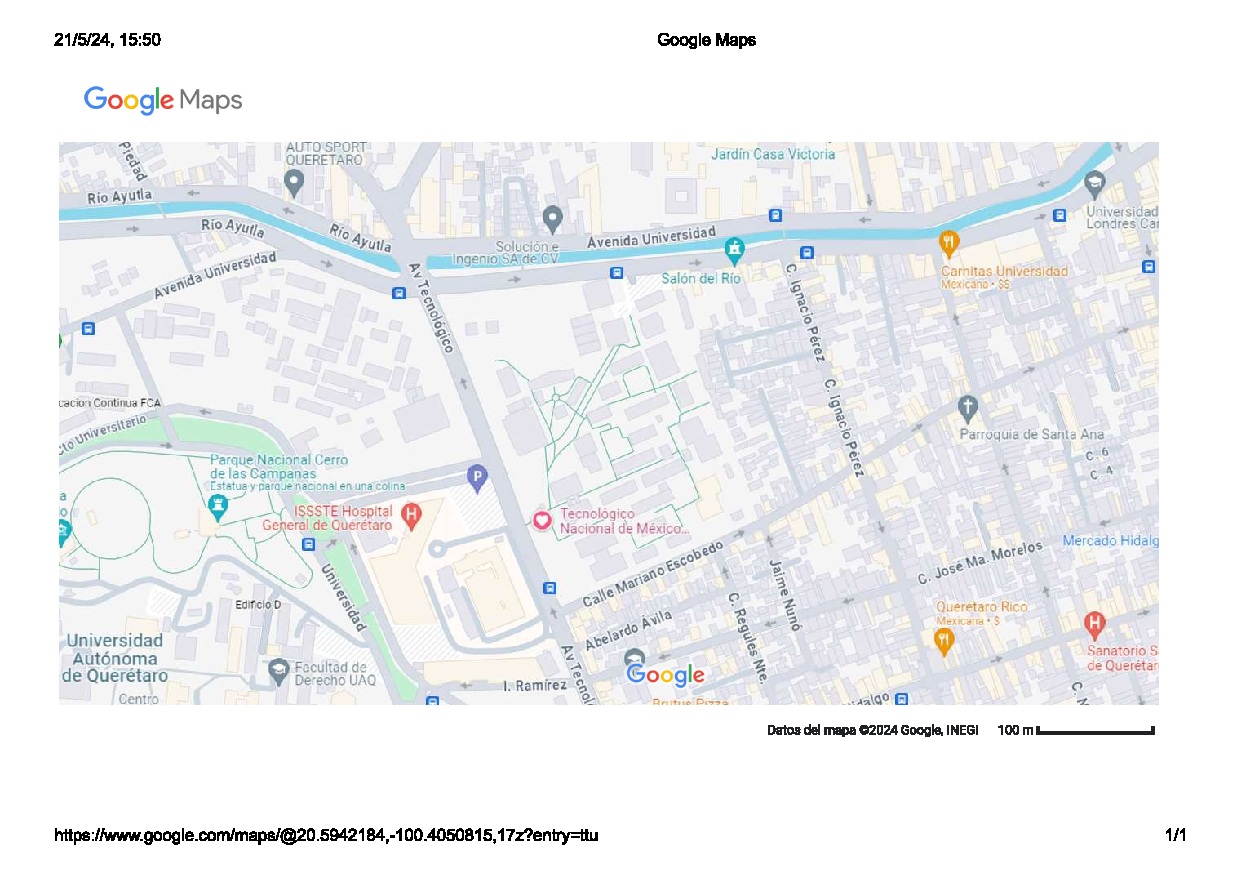
\includegraphics[trim = {12mm 20mm 10mm 14mm},clip,scale=0.45]{22/Img/planoDeUbicacionEnMaps.pdf}
        \caption{Mapa geográfico de Google Maps}
        \label{fig:croquisGoogle}
    \end{figure}
    
    
    En la figura \ref{fig:croquisPlano} se observa un croquis interno creado y proporcionado por el departamento de Planeación en la oficina de Construcción y Equipamiento, este plano plasma una imagen detallada del instituto en donde se observa cada área y la distribución del plantel. 
    \begin{figure}[H] 
        \centering
        \includegraphics[trim = {0.001mm 0.001mm 0.001mm 0.001mm},clip,scale=0.06]{22/Img/croquisPlanoITQ.pdf}
        \caption{Croquis proporcionado por el instituto}
        \label{fig:croquisPlano}
    \end{figure}
    
    \begin{figure}[H] 
        \centering
        \includegraphics[trim = {12mm 20mm 10mm 14mm},clip,scale=0.45]{22/Img/medidasEdificio.pdf}
        \caption{Plano con las medidas del edificio C y distancia de la salida más cercana}
        \label{fig:medidas}
    \end{figure}
    
    
    
    \begin{figure}[H] 
        \centering
        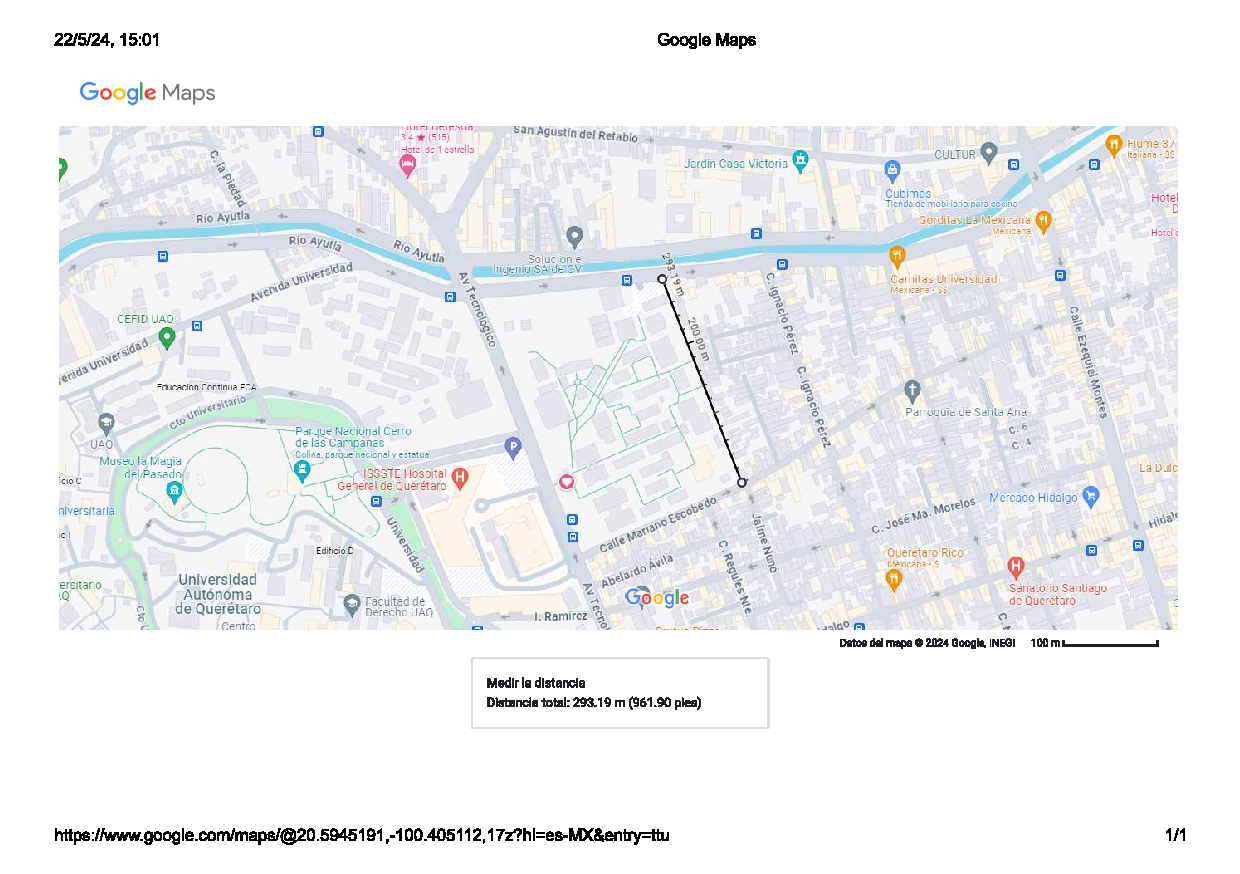
\includegraphics[trim = {12mm 20mm 10mm 14mm},clip,scale=0.45]{22/Img/evidenciaDeMedicionEnMaps.pdf}
        \caption{Medición de la institución por la parte posterior}
        \label{fig:medicionMaps}
    \end{figure}
    
    En la imagen \ref{fig:medicionMaps} podemos observar la evidencia de como se midió la parte posterior destitución utilizando el sitio web de Google Maps, utilizando la metodología siguiente: Primeramente, se buscó la dirección del instituto en el sitio web, posterior a ubicarla dirigimos el cursor a la parte inferior izquierdo de la pantalla, a la parte de capas, se seleccionó y consecutivamente se buscó la opción Medir, utilizamos esta opción y se colocó el cursor en el inicio de la parte  colindante con la calle Mariano Escobedo pegado a las casas, en consiguiente se colocó el cursor en la parte colindante con Avenida Universidad en donde automáticamente el sitio web nos dio las medidas. Como se observa, la medición que nos dio la aplicación fue de 293.19 que es la parte trasera, para las demás medidas utilizamos la misma metodología y las medidas contundentes son las siguientes; Por la parte frontal colindante con Tecnológico nos dio una medición de 349.32 m; La parte lateral Colindante con Universidad fue de 236.54 m, mientras que para la colindante con Mariano Escobedo fue de 232.84 m; Y ya anteriormente mencionado el perímetro posterior de la institución fue de 293.19 m.
    
    Cabe mencionar que estas medidas no son totalmente exactas y siempre habrá una variación, dado que esta página solo es una ayuda para nuestra referencia y por ello estos datos no pueden ser considerados para un trabajo de calidad. Con esto en mente, se tomó la decisión de tomar nuestras propias medidas, la metodología de esta aplicación fue realizar nuestras medidas con ayuda de un flexómetro de 10 m. Con este material se inició las medidas por todo el perímetro de la institución, tomando cada medida de 10 en 10 y algunas menores, dado que las mediciones no se podían medir por completo, o tan solo por el hecho que el perímetro no tiene un valor cerrado, por ello cada medida que tomábamos la íbamos anotando y al final se sumó todos los valores. Ya con estos valores logramos tomar una medida lo más precisa posible, aunque se debe tomar en cuenta que estos datos aun así no pueden ser exactos, dado que ni los materiales ni los métodos son los mejores.
    
    Con este método de medición los valores obtenidos fueron los siguientes: 348.44 m sobre Tecnológico, 250.89 m por la Av. Universidad, 231.54 m  colindantes con Mariano Escobedo; y por último 292.78 m en la parte posterior.
    
    %Salon largo : 45.38 m
    %Largo:9.54 m
    \subsubsection{Análisis de riesgos}
    
    \begin{figure}[H] 
        \centering
        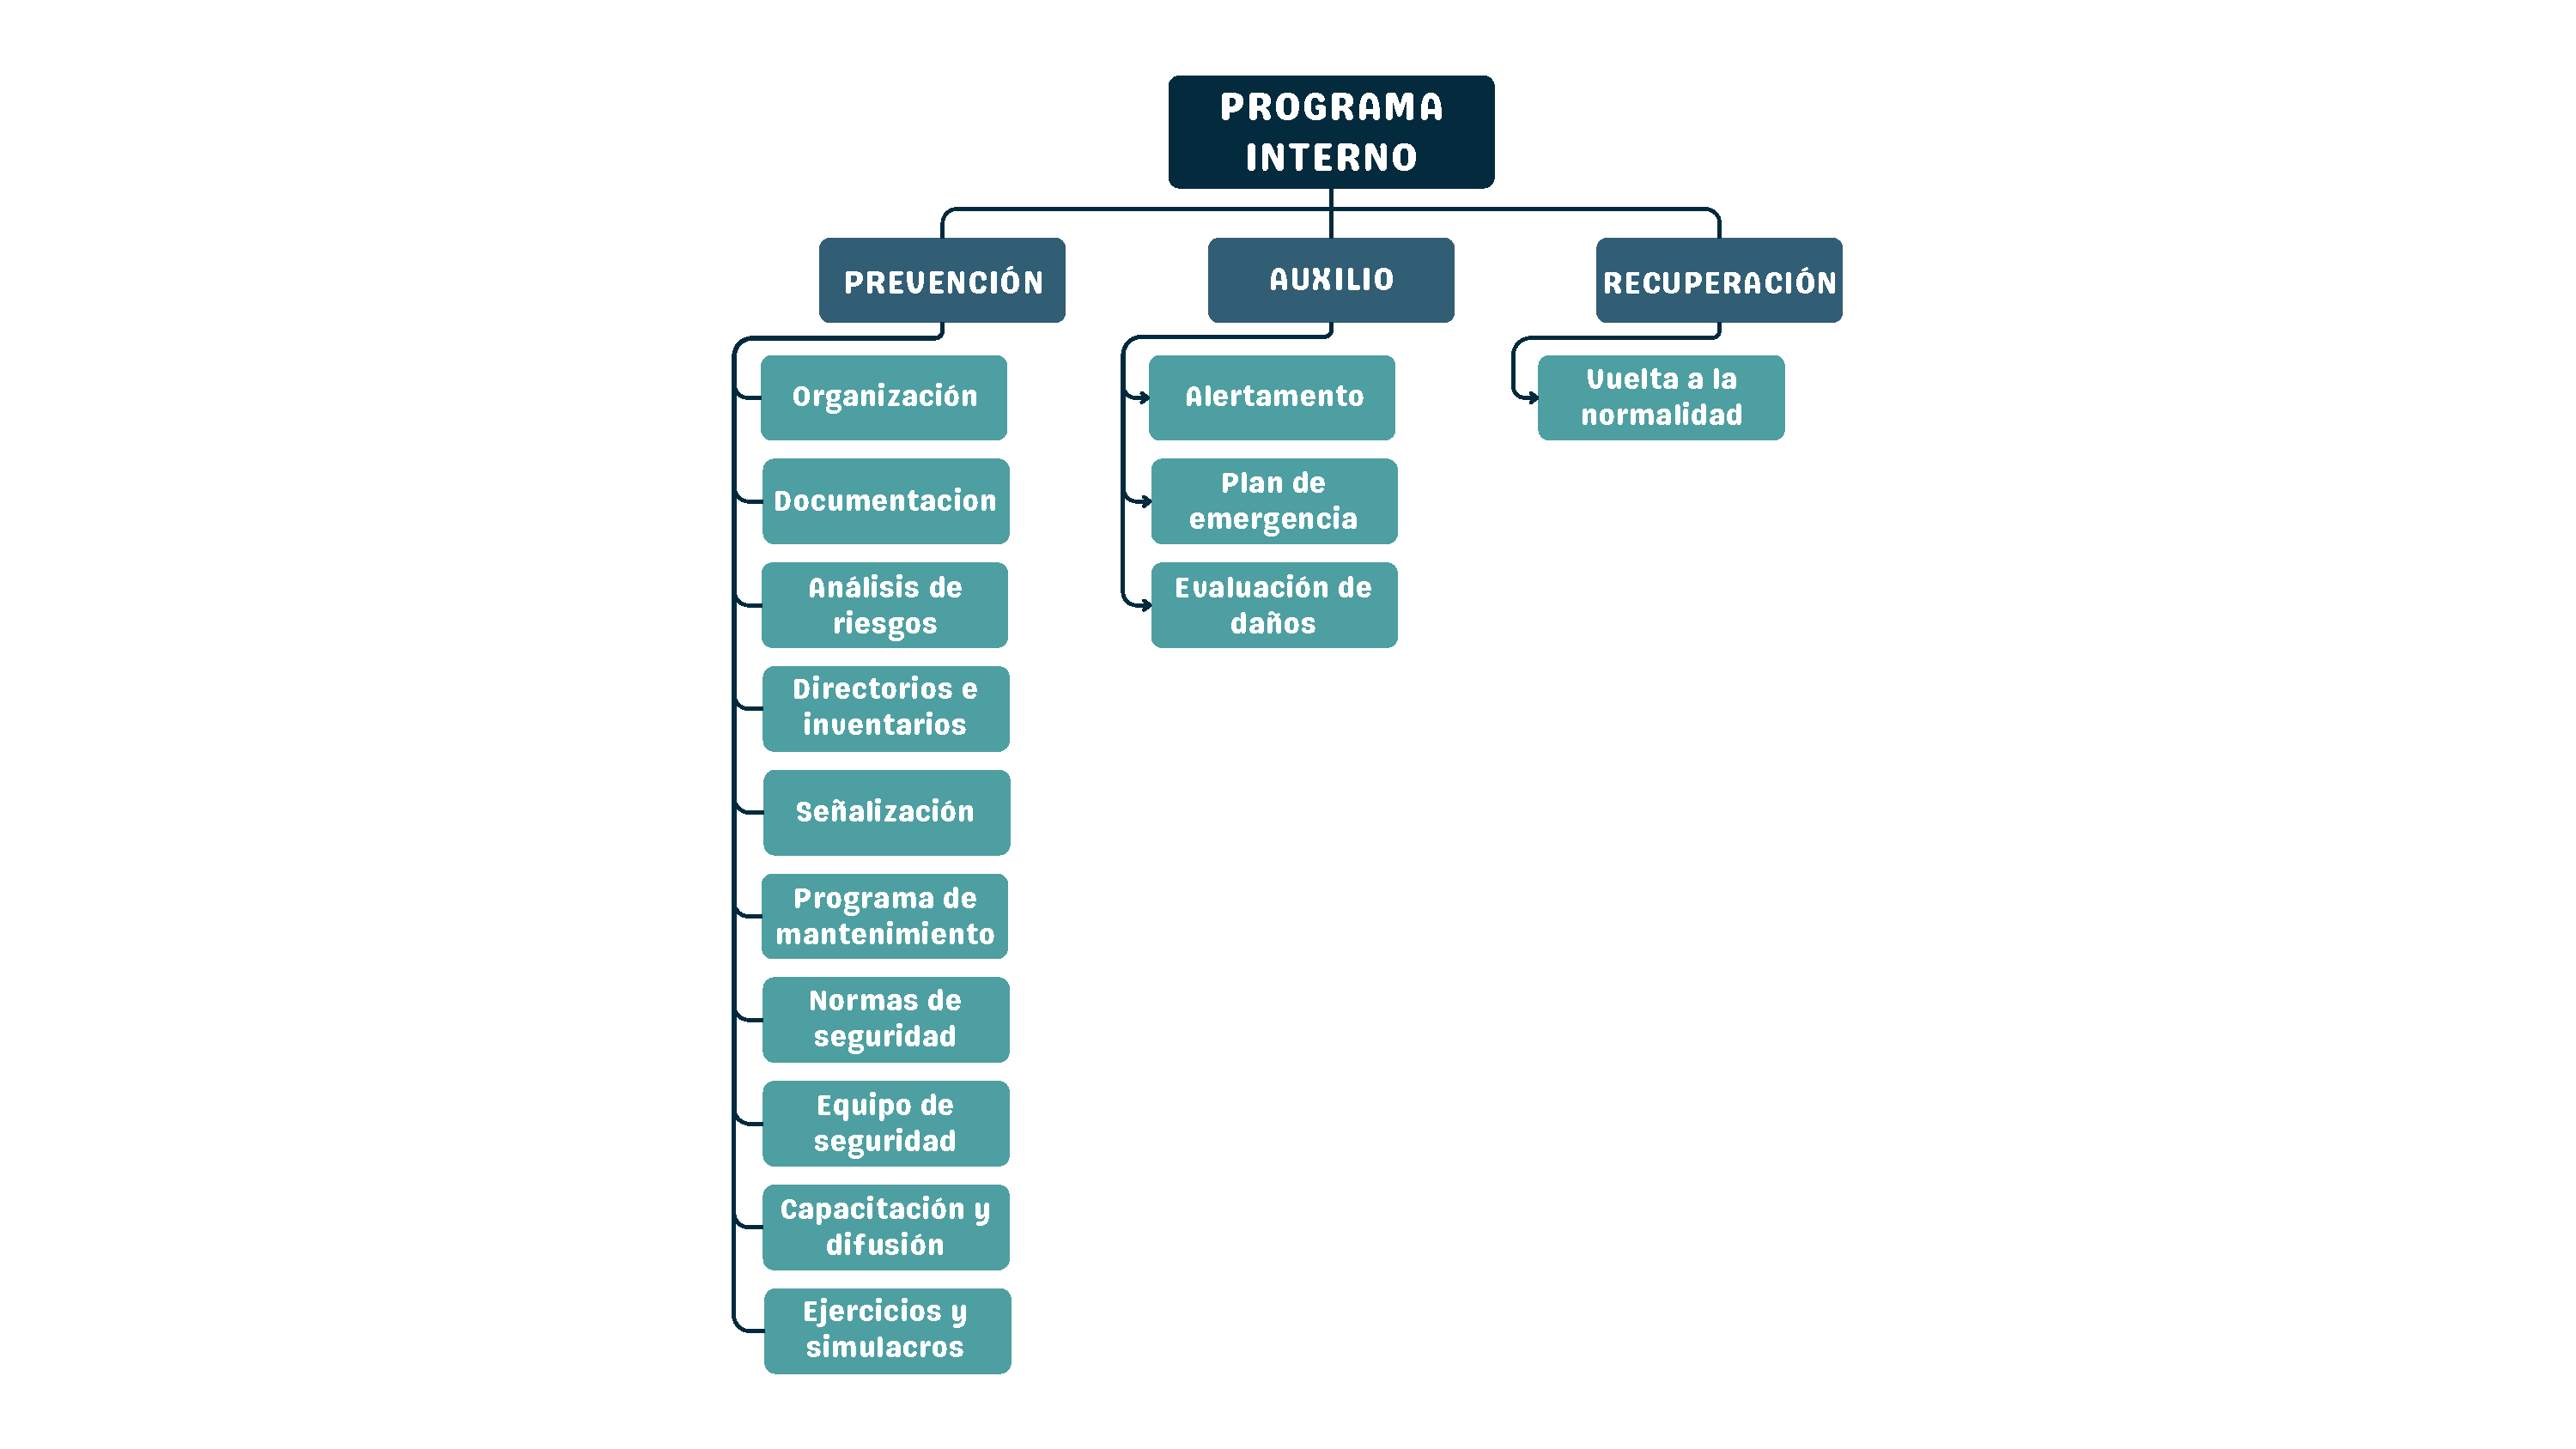
\includegraphics[trim = {140mm 15mm 140mm 15mm},clip,scale=0.4]{22/Img/programaInterno.pdf}
        \caption{Diagrama para la identificación de riesgos y acciones}
        \label{fig:dig}
    \end{figure}
    
    \subsubsection{Identificación de riesgos internos}
    
    
    \begin{figure}[H] 
        \centering
        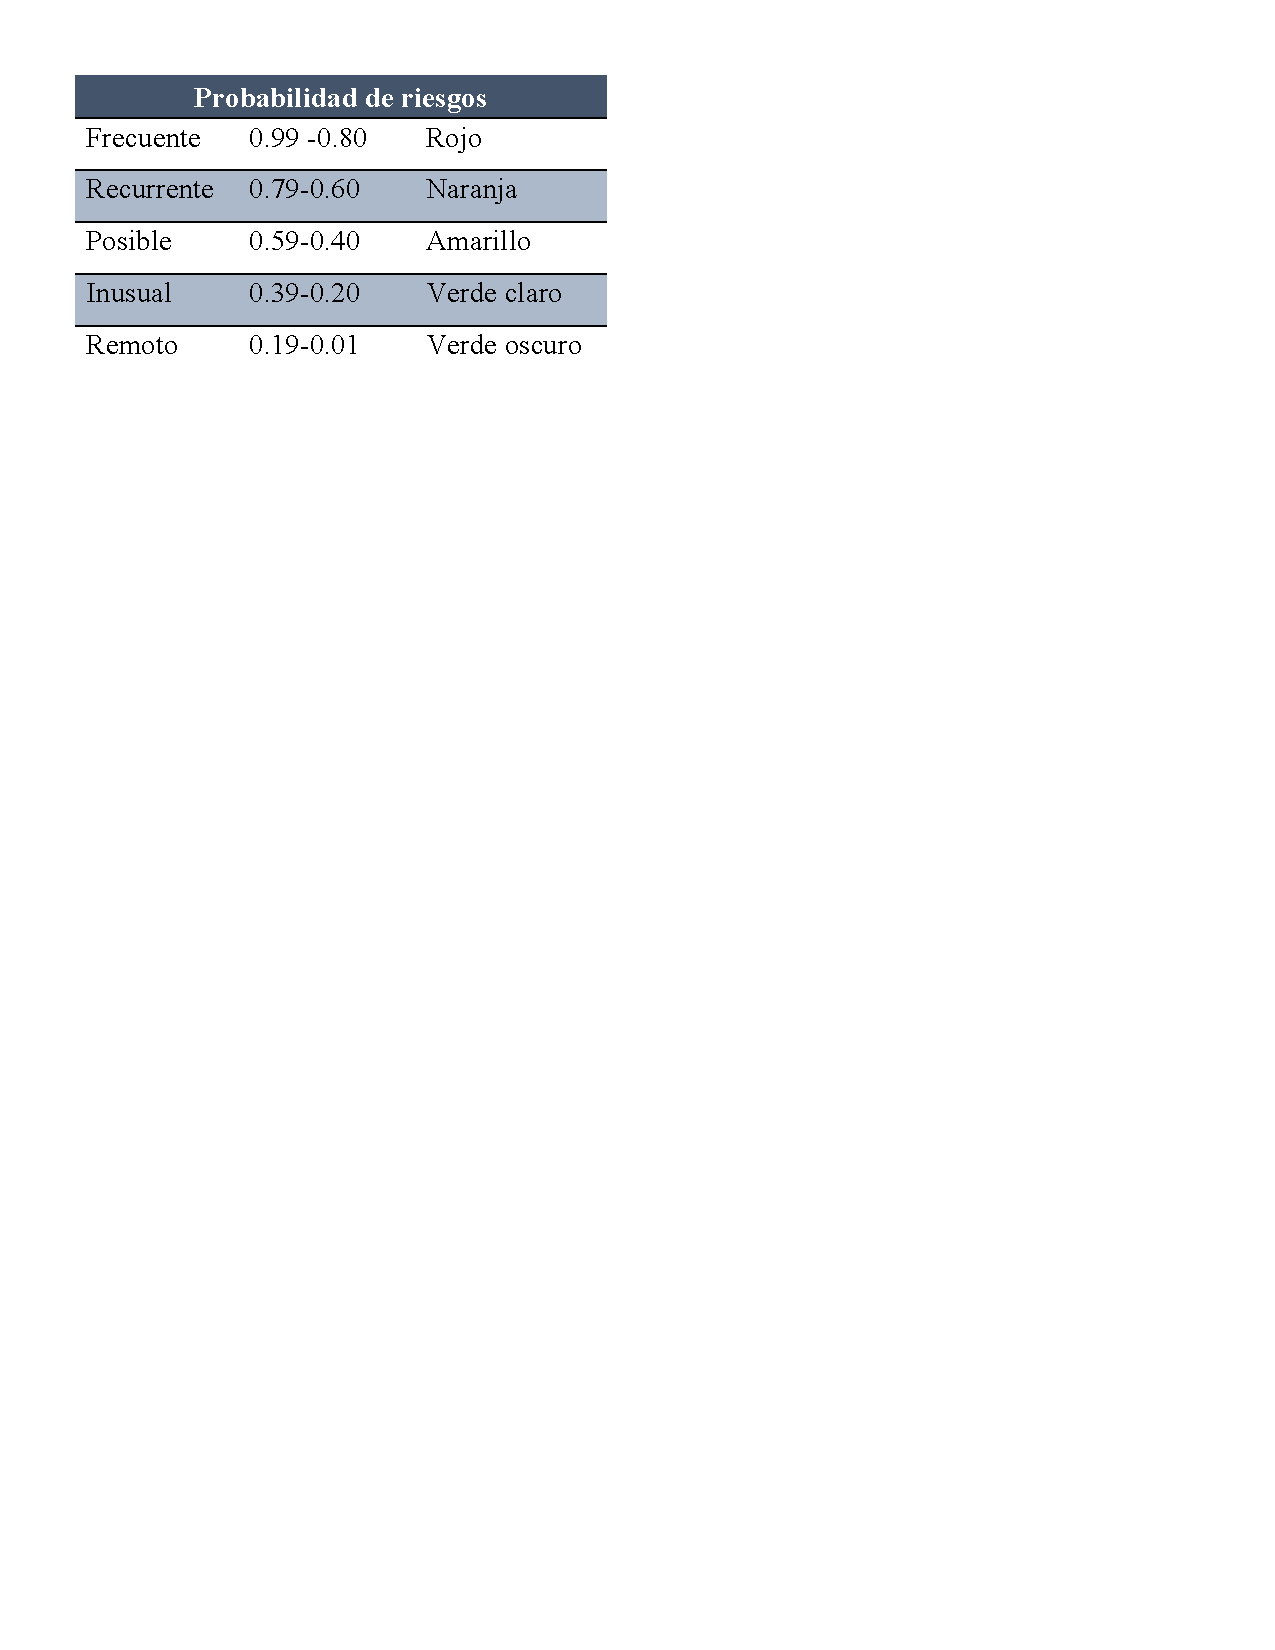
\includegraphics[trim = {10mm 215mm 100mm 10mm},clip,scale=0.7]{22/Img/riesgosPorProbabilidad.pdf}
        \caption{Riesgos con diferentes niveles y colores para distinguir la probabilidad}
        \label{fig:prob}
    \end{figure}
    
    \begin{figure}[H] 
        \centering
        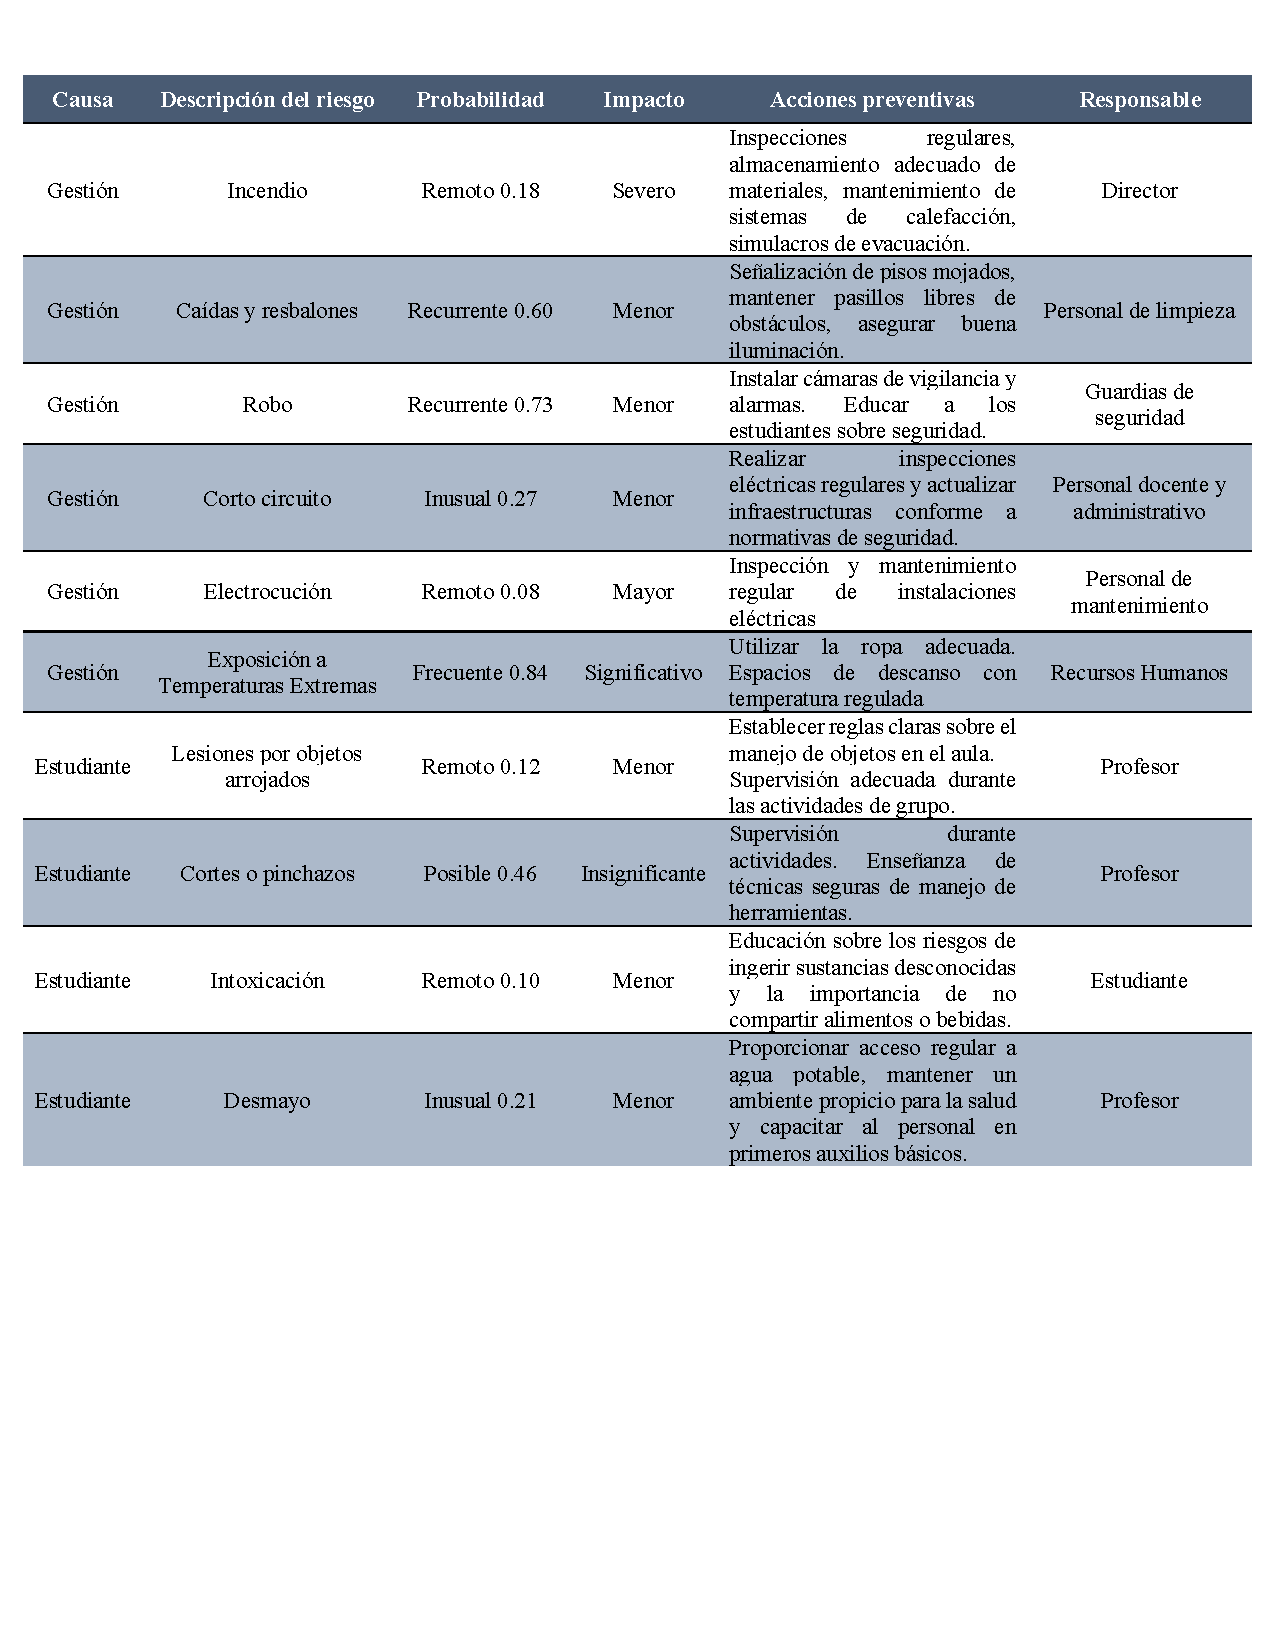
\includegraphics[trim = {1mm 70mm 1mm 10mm},clip,scale=0.38]{22/Img/riesgosInternos.pdf}
        \caption{Descripción de los riesgos al realizar las activida-
    des más comunes y de riesgo dentro de la empresa}
        \label{fig:ideIn}
    \end{figure}
    
    \subsubsection{Identificación de riesgos externos}
    
    \begin{figure}[H] 
        \centering
        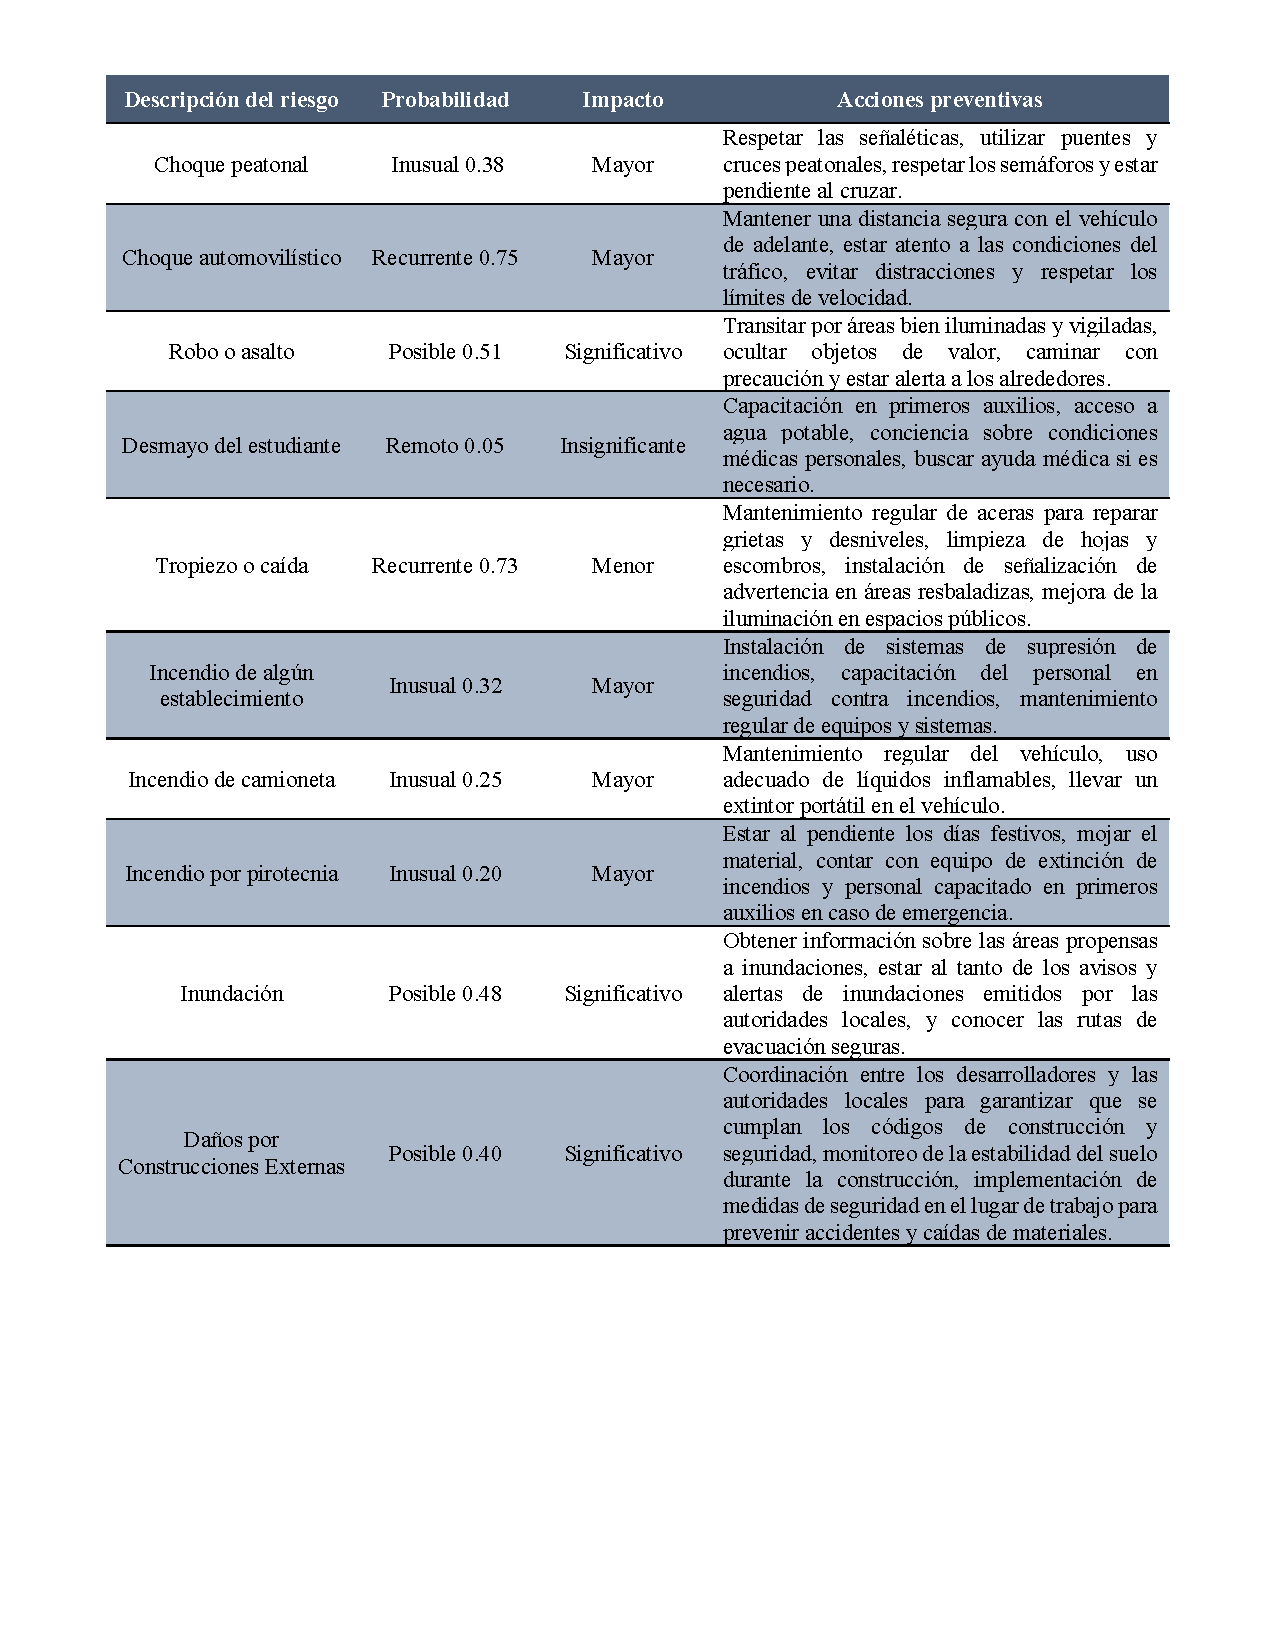
\includegraphics[trim = {15mm 60mm 15mm 10mm},clip,scale=0.41]{22/Img/riesgosExternos.pdf}
        \caption{Descripción de los riesgos externos}
        \label{fig:ideEx}
    \end{figure}
    \subsubsection{Programa de actividades de prevención y auxilio}
    
    
    \subsubsection{Plan de acción}
    
    
    \begin{figure}[H]
        \centering
        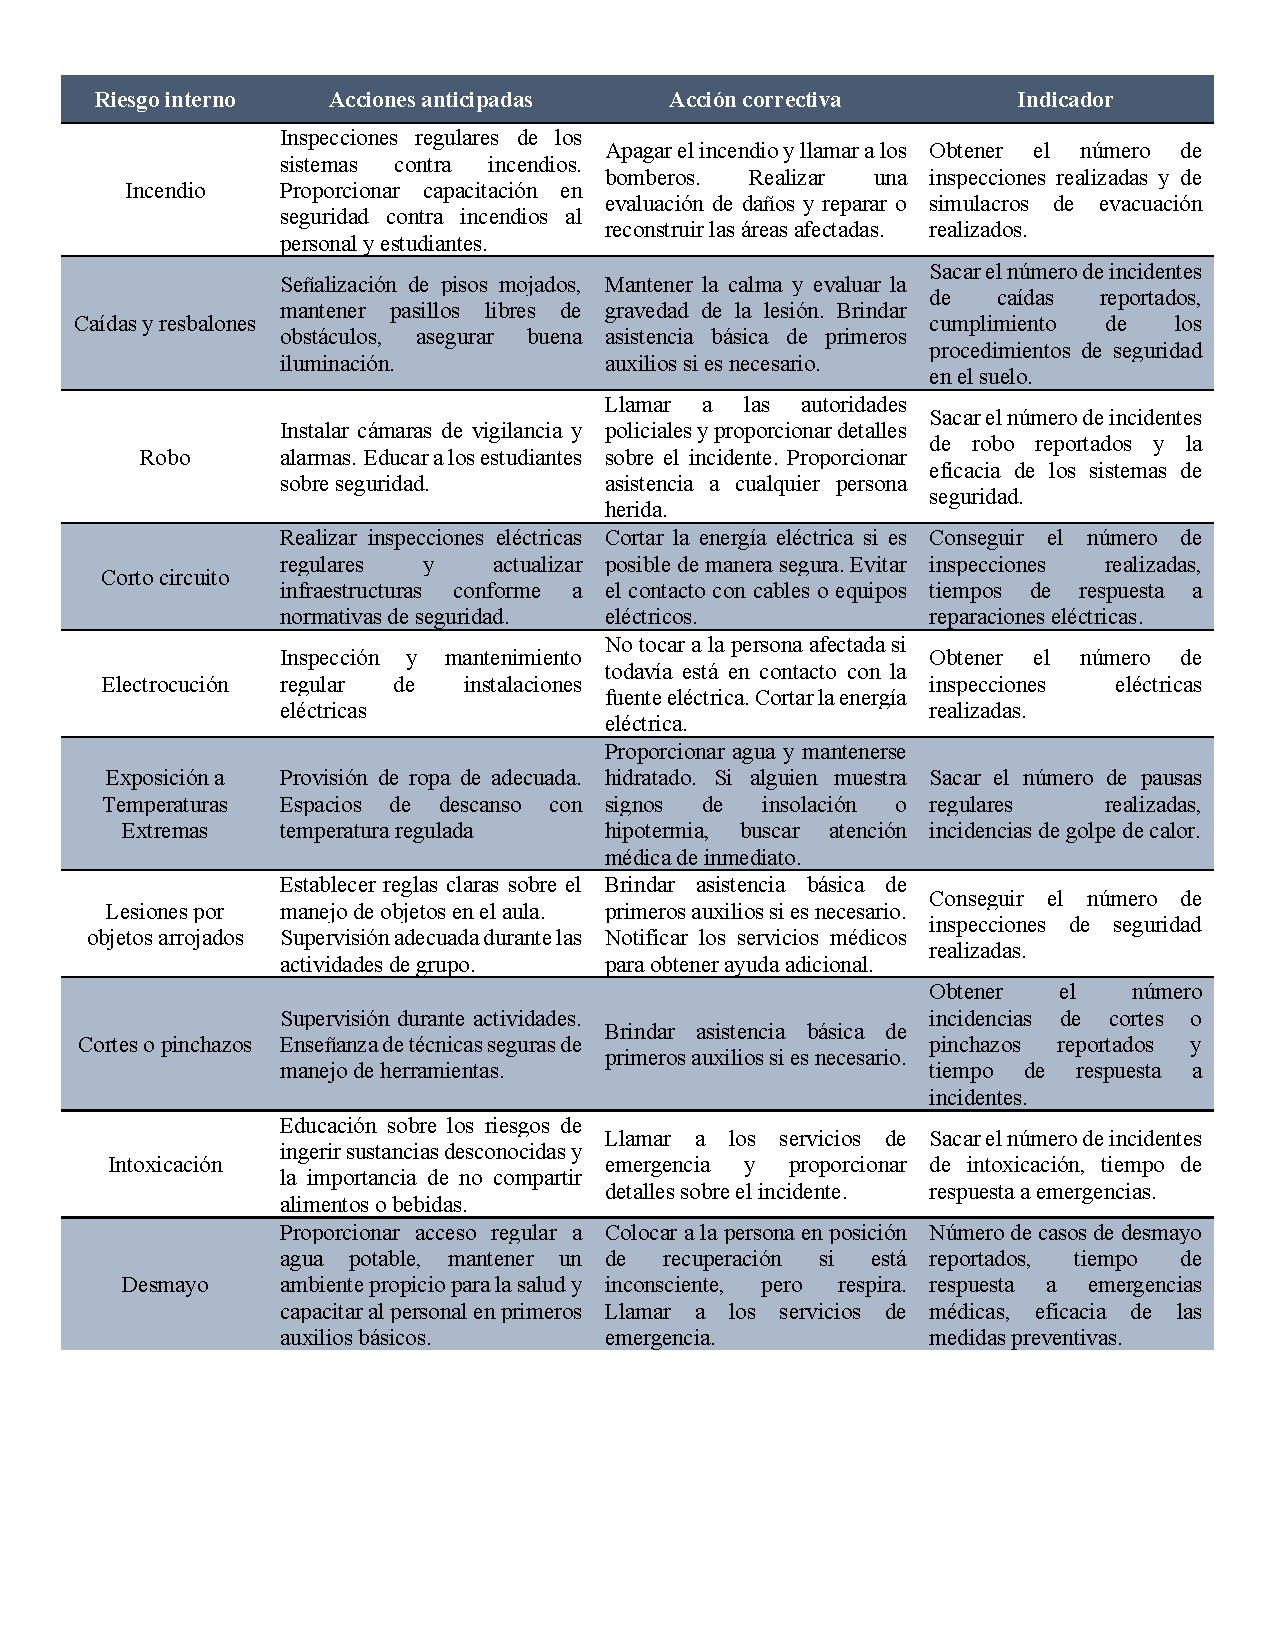
\includegraphics[trim = {10mm 40mm 10mm 10mm},clip,scale=0.41]{22/Img/riesgosInternos2.pdf}
        \caption{Descripción de las acciones anticipadas y correctivas ante un riesgo interno }
        \label{fig:accionAntInterno}
    \end{figure}
    
    \begin{figure}[H]
        \centering
        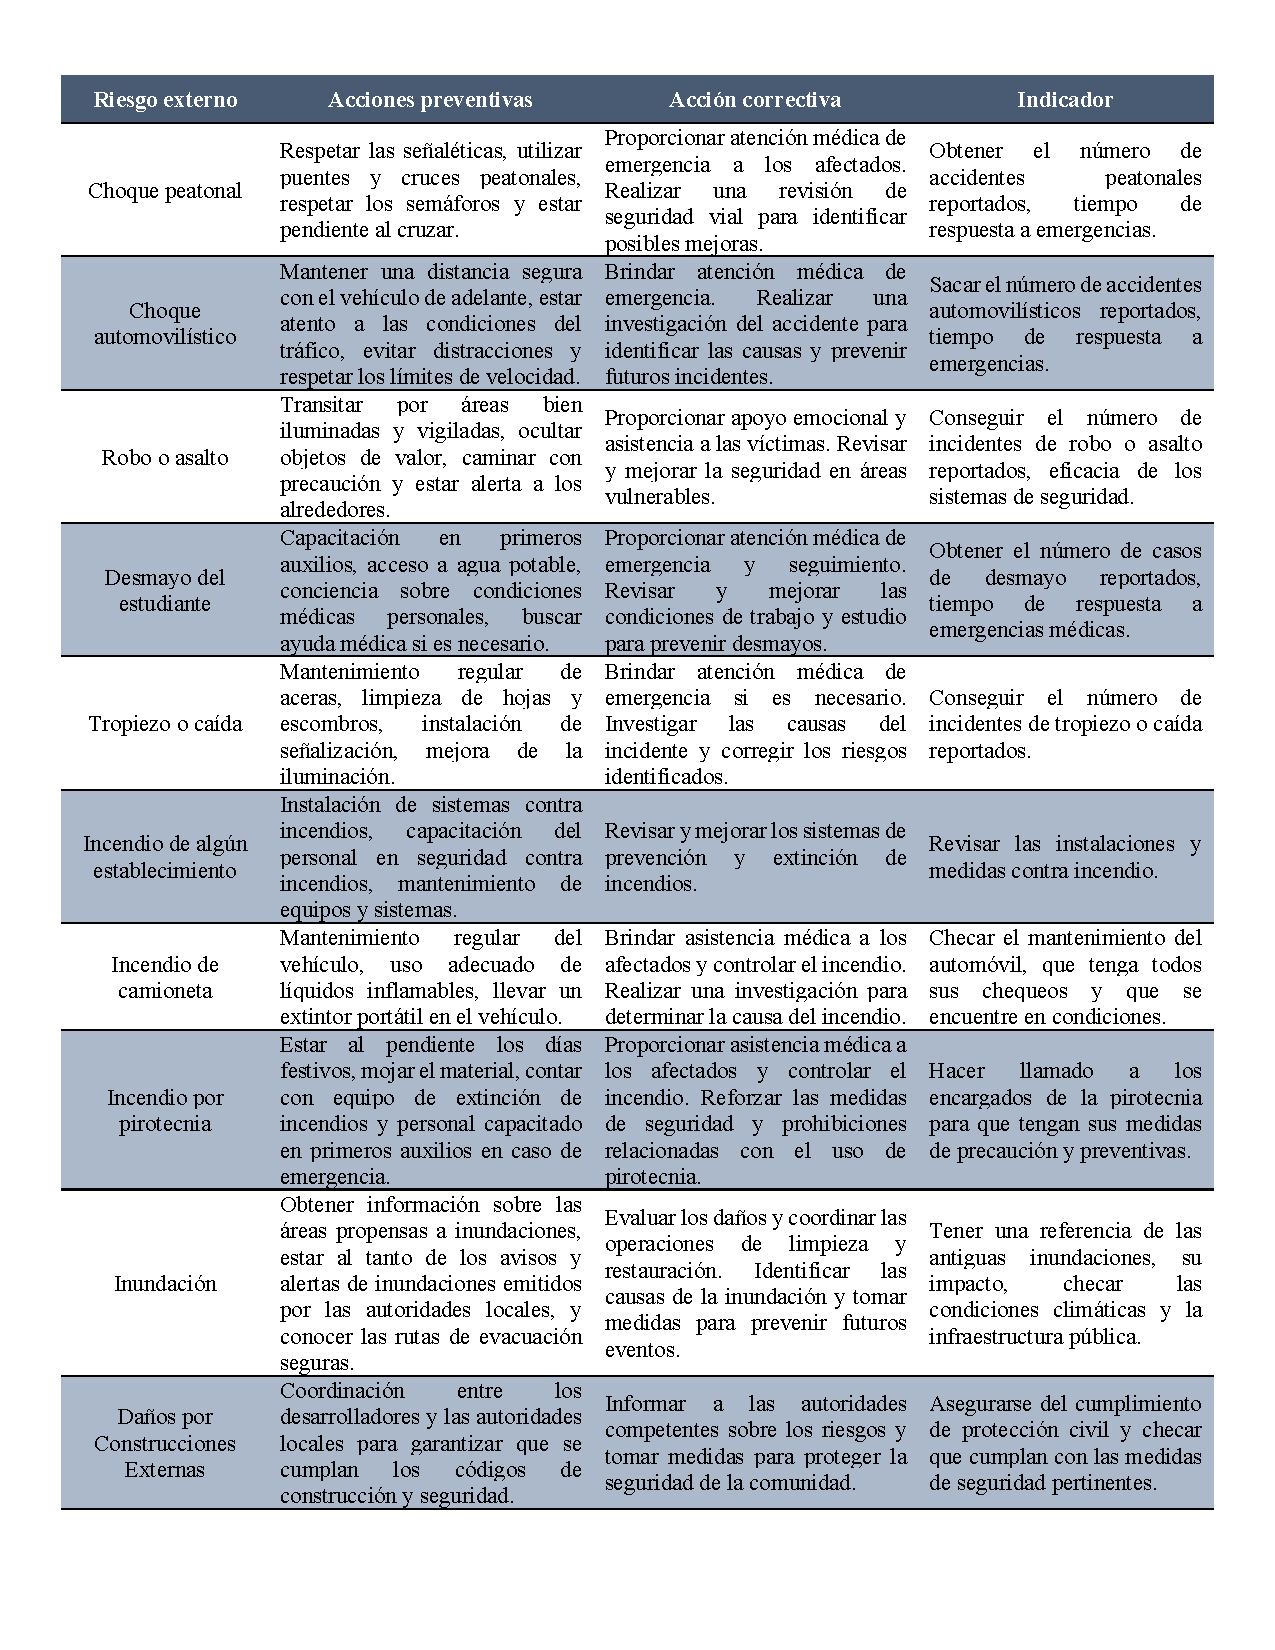
\includegraphics[trim = {10mm 20mm 10mm 10mm},clip,scale=0.41]{22/Img/riesgosExternos2.pdf}
        \caption{Descripción de las acciones anticipadas y correctivas ante un riesgo externo}
        \label{fig:accionAnti}
    \end{figure}
    
    
    
    
    \subsubsection{Identificación de capacidades}
    
    
    
    \subsubsection{Plano de localización de recursos}
    
    % \begin{figure}[H]
         %   \centering
          %  \includegraphics[trim = {20mm 25mm 20mm 12mm},clip,scale=0.3]%{22/Img/PlanoLocalizaciónRecursos.pdf}
    %        \caption{Plano del establecimiento de los recursos en materia de seguridad.}
     %       \label{fig:PlanoLocalizaciónRecursos}
      %  \end{figure}
    
    \subsubsection{Identificación de apoyos externos}
    \begin{figure}[H]
        \centering
        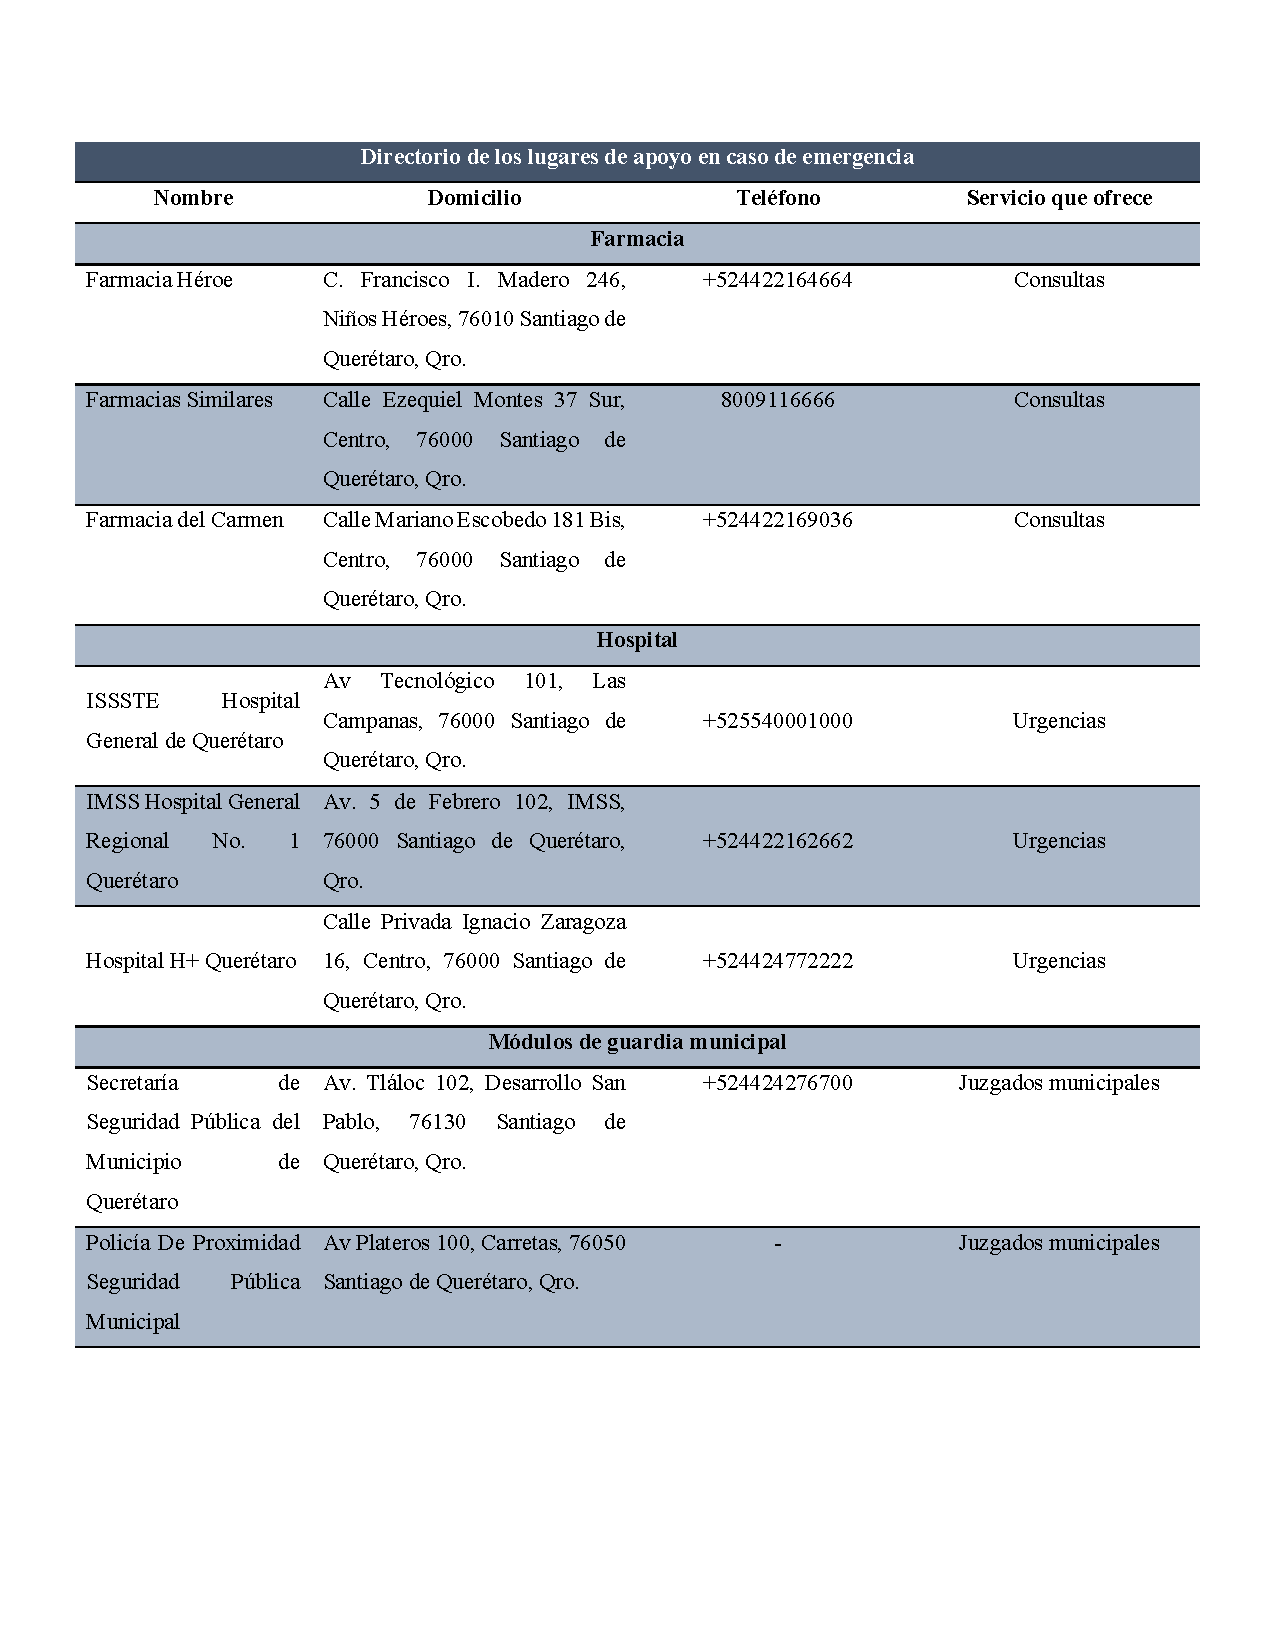
\includegraphics[trim = {10mm 45mm 10mm 15mm},clip,scale=0.4]{22/Img/apoyosExt.pdf}
        \caption{ Lugares que servirán de apoyo en una situación de emergencia.}
        \label{fig:apoyosExt}
    \end{figure}
    
    \subsubsection{Identificación de puntos de reunión}
    
    
    \begin{figure}[H]
        \centering
         \includegraphics[trim = {0.001mm 0.001mm 0.001mm 0.001mm},clip,scale=0.07]{22/Img/localizacionDePuntosDeReunion.pdf}
        \caption{Zona segura en caso de una evacuación de emergencia.}
        \label{fig:puntosDeReunión}
    \end{figure}
    
    
    \begin{figure}[H]
        \centering
        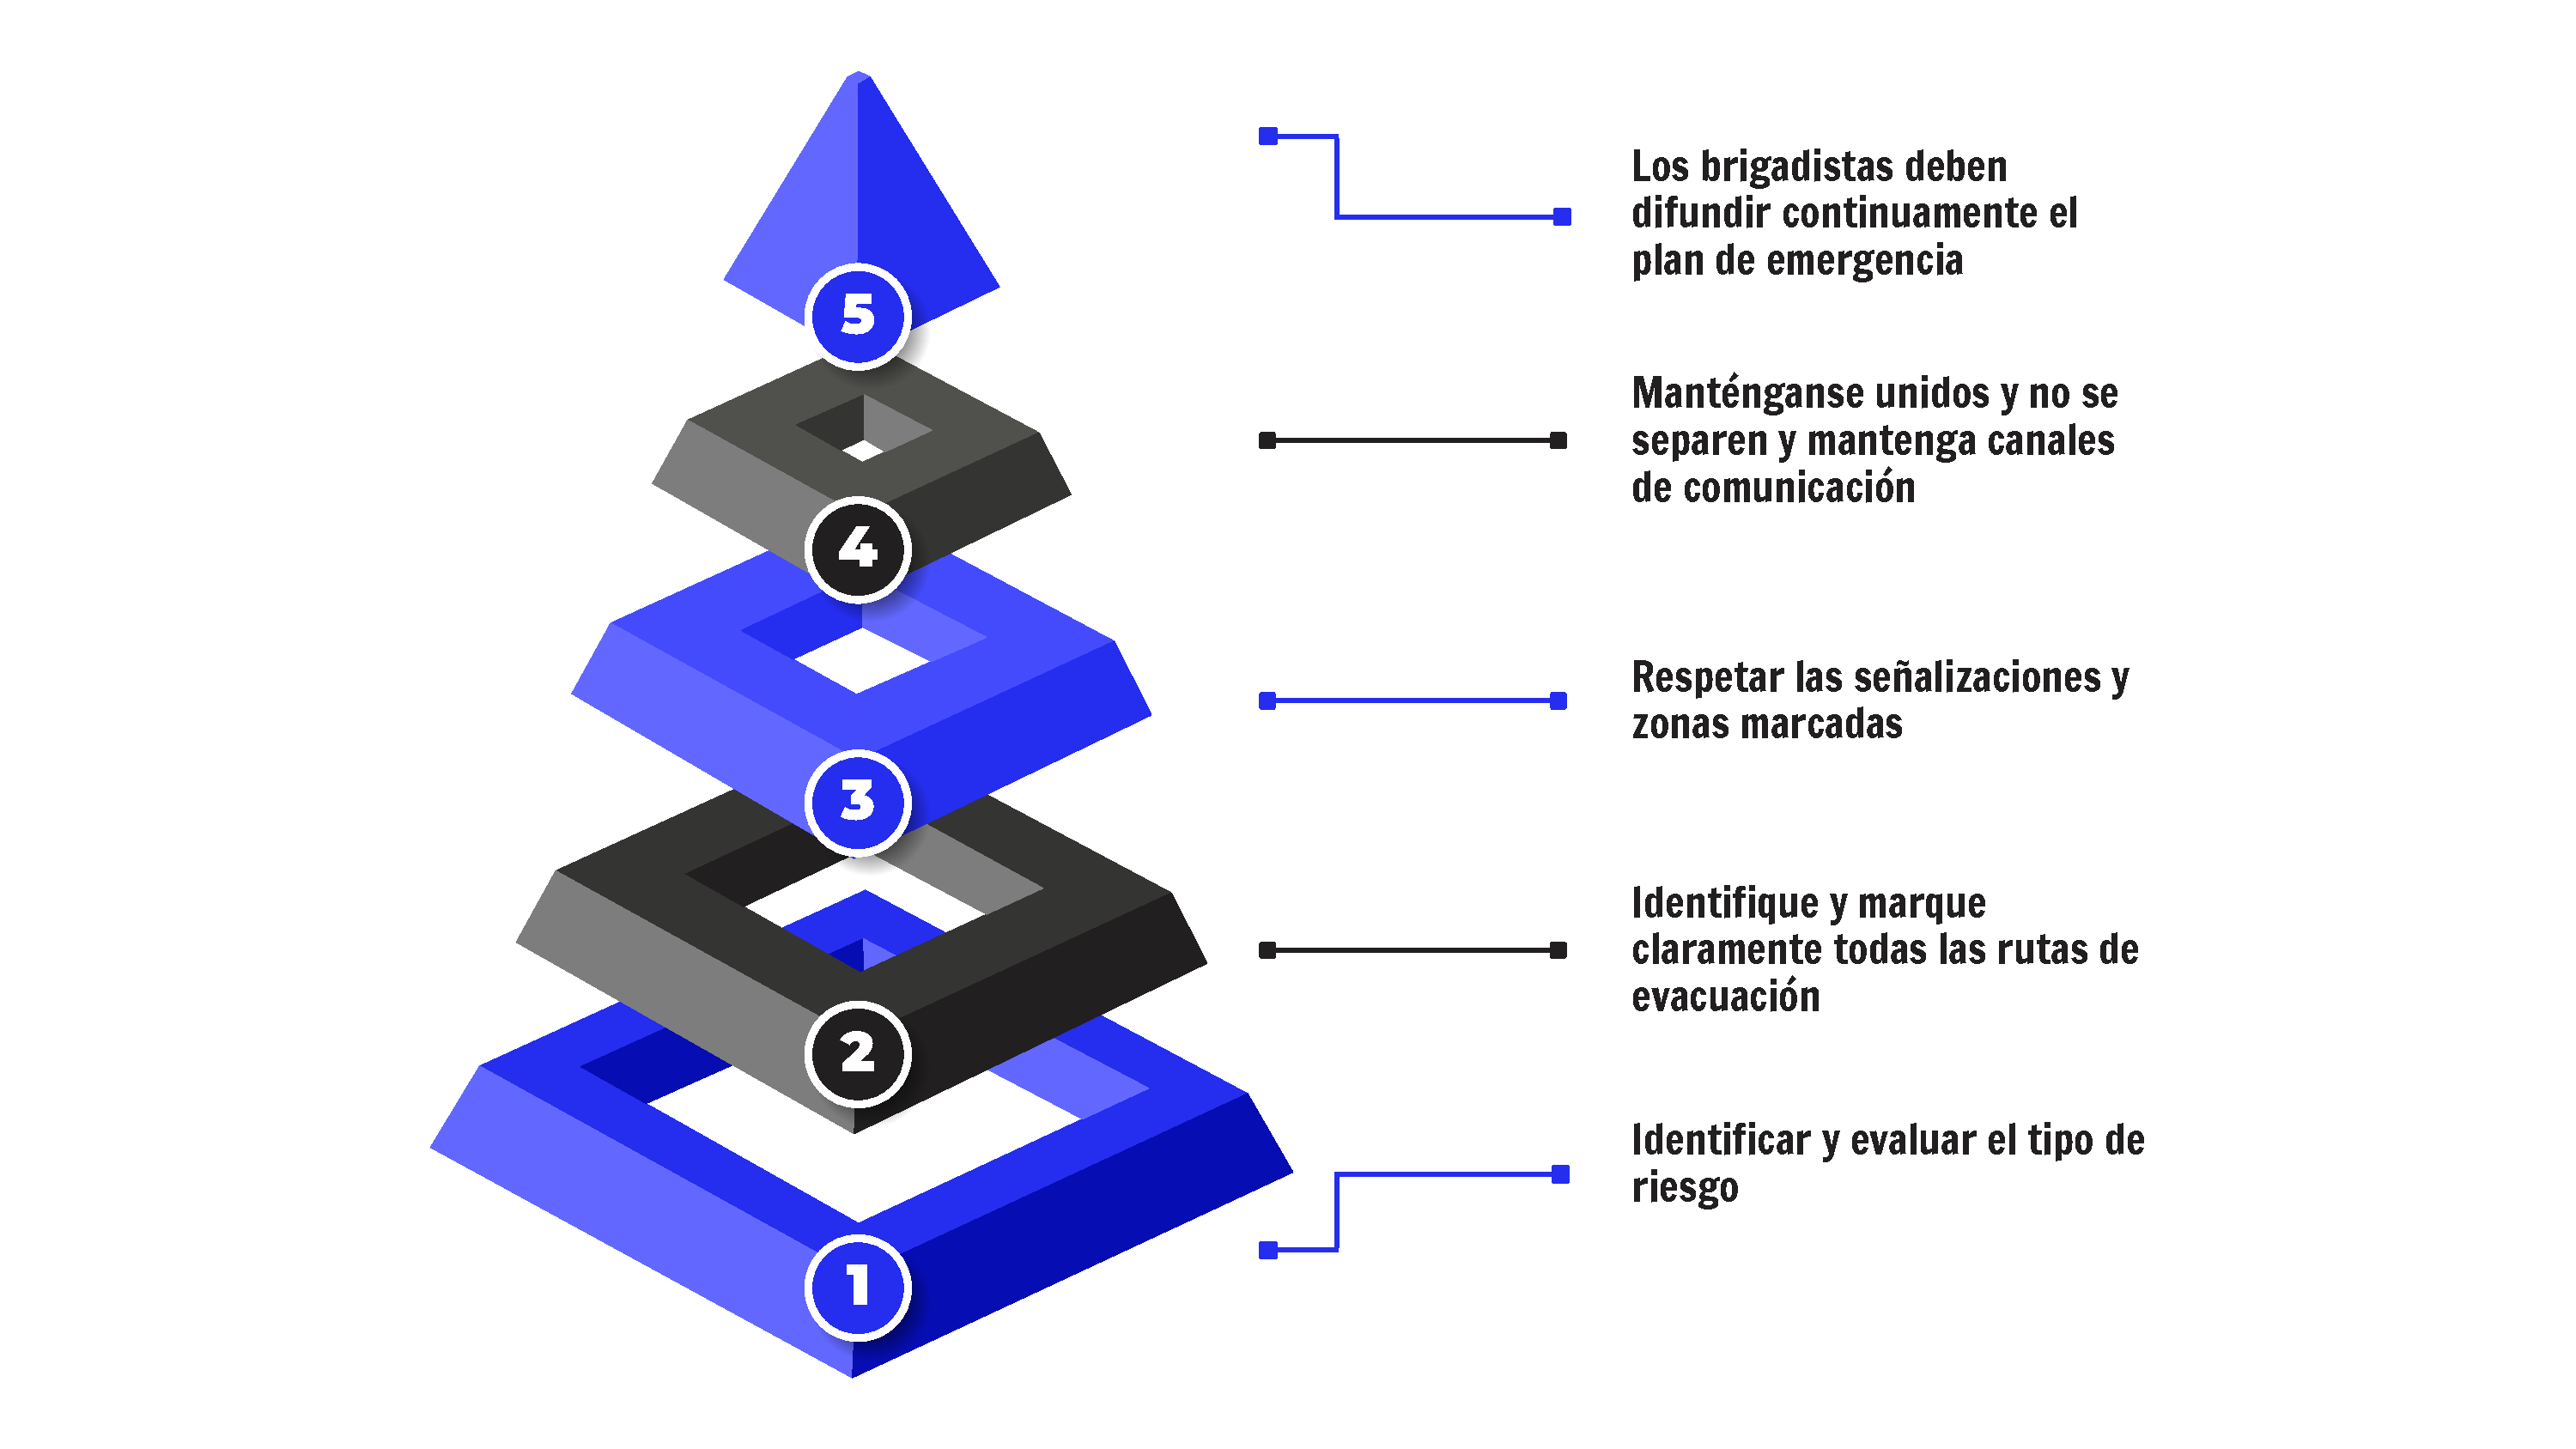
\includegraphics[trim = {60mm 10mm 60mm 10mm},clip,scale=0.25]{22/Img/repliegue.pdf}
        \caption{El repliegue que se realiza cunado las condiciones del inmueble son adecuadas.}
        \label{fig:planDeRepliege}
    \end{figure}
    
    
    
    \begin{figure}[H]
        \centering
        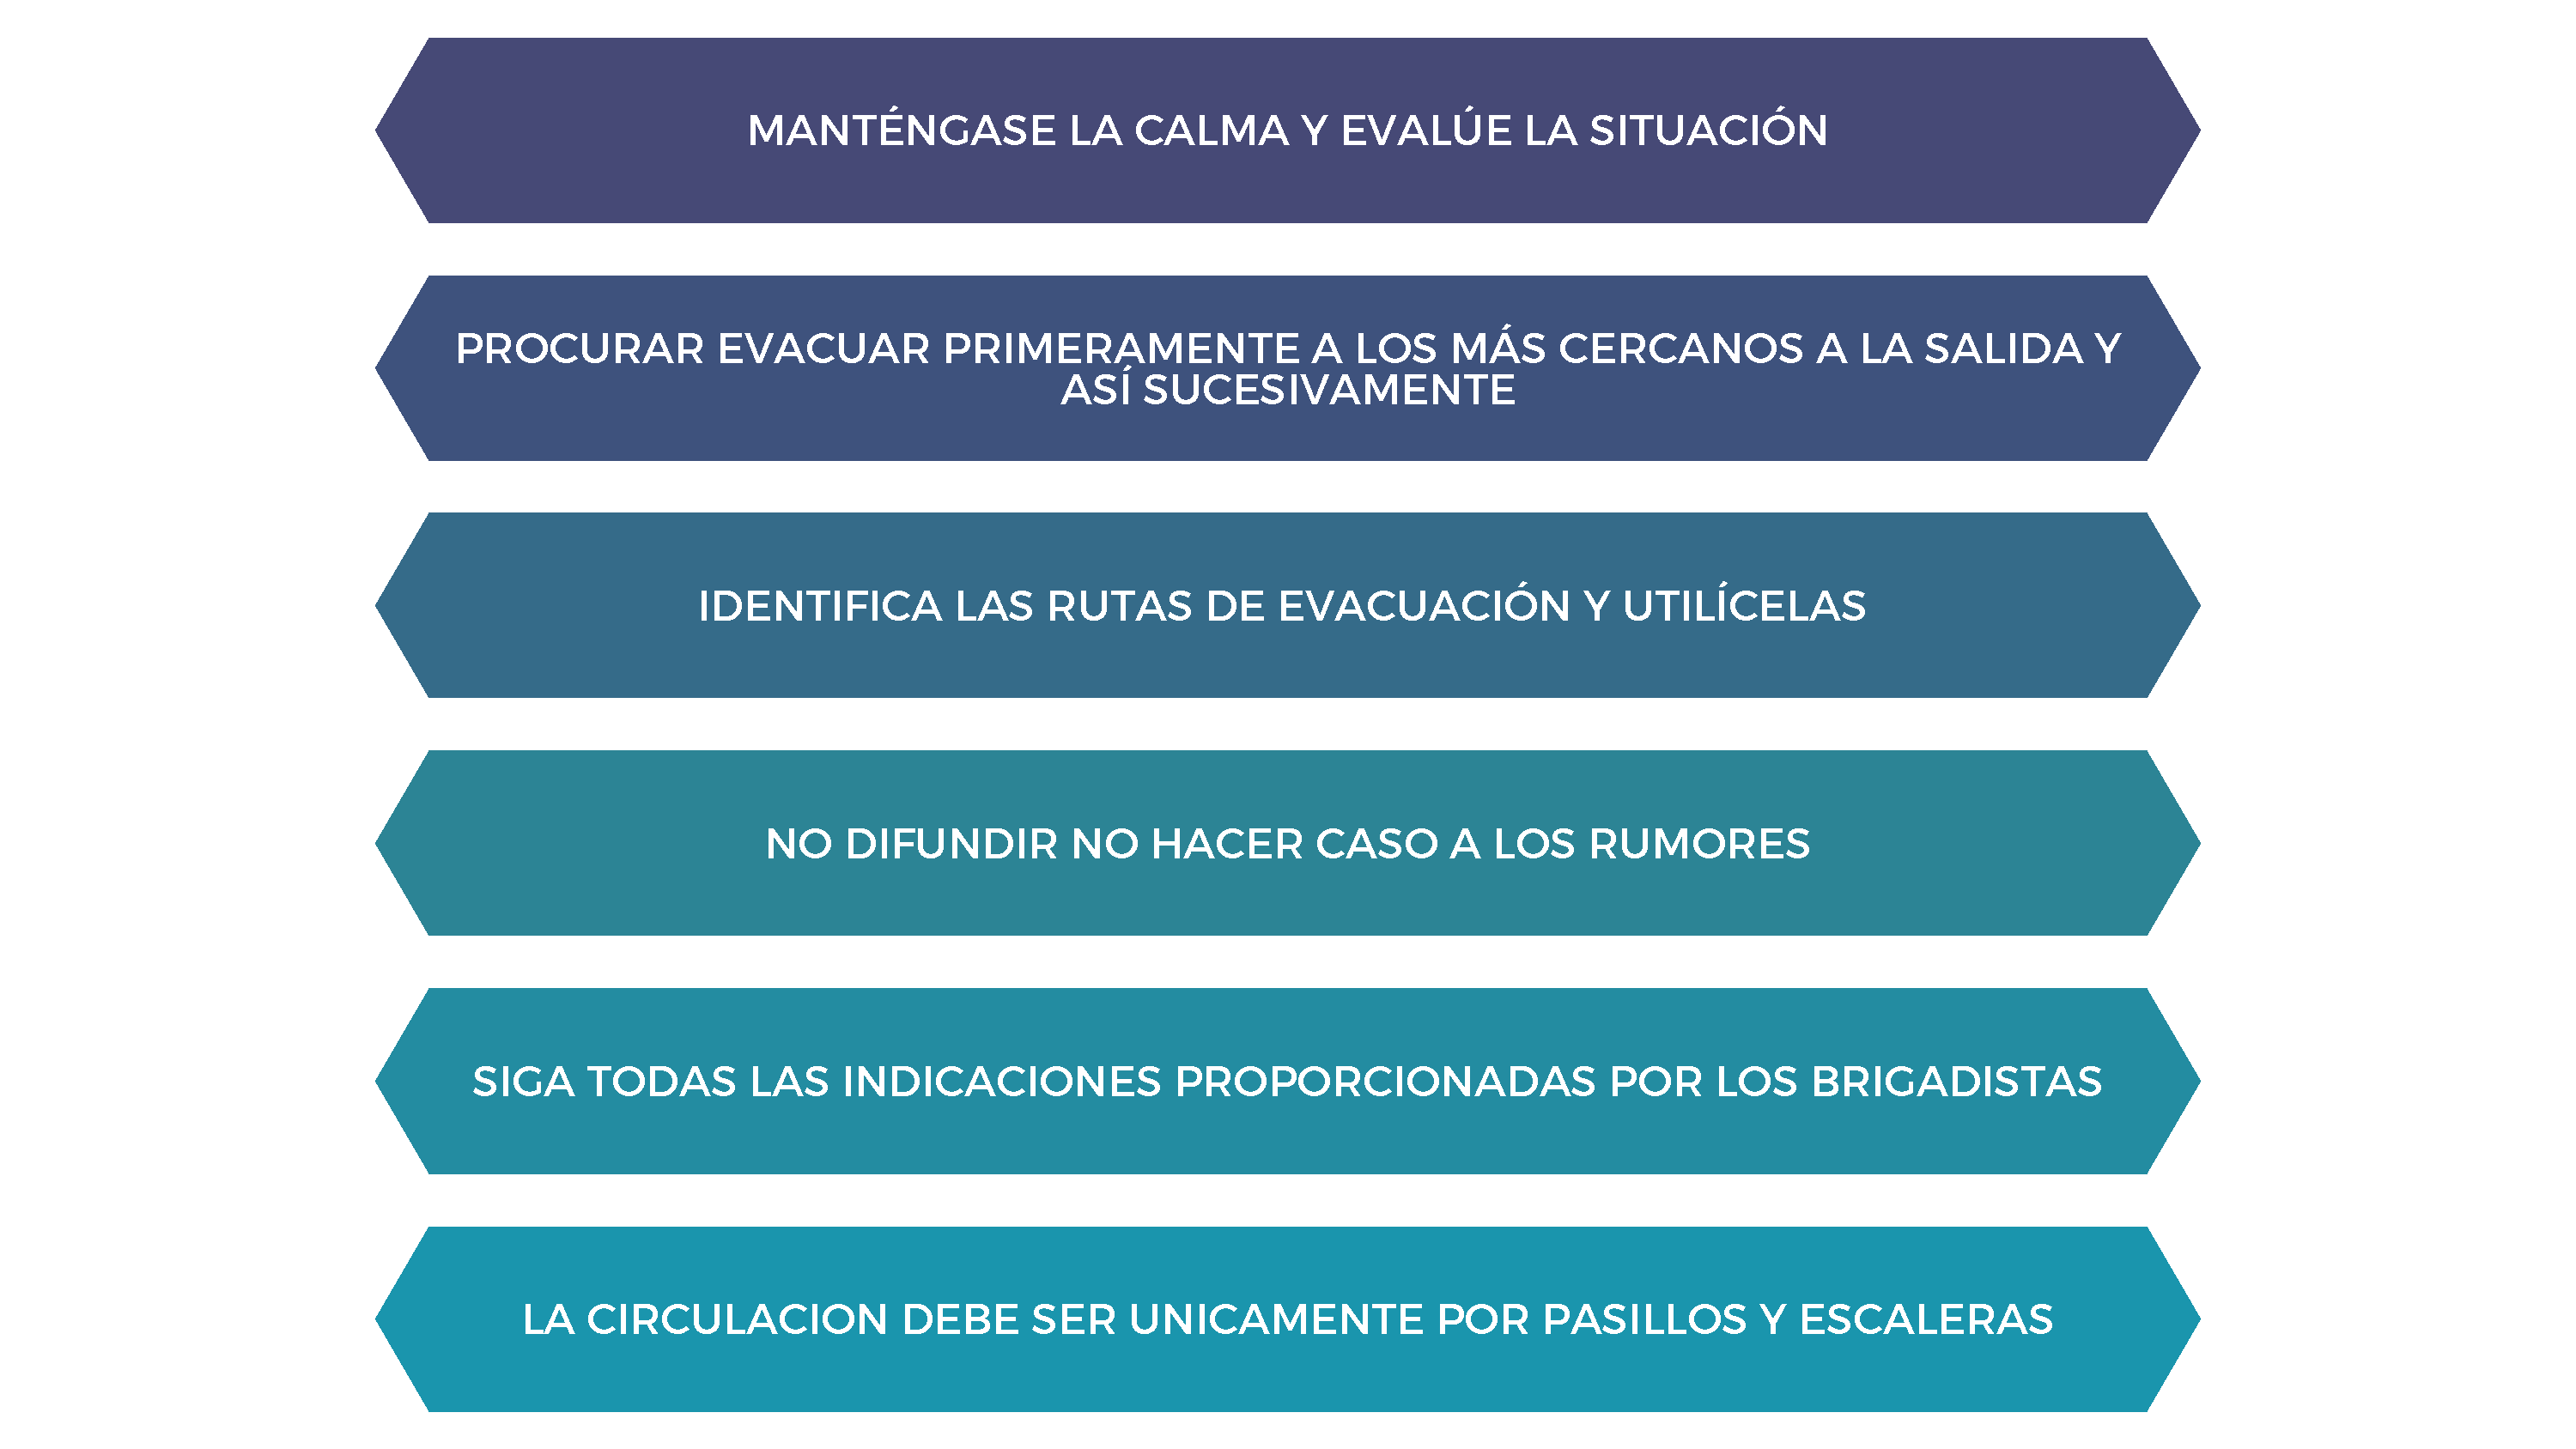
\includegraphics[trim = {60mm 10mm 60mm 10mm},clip,scale=0.23]{22/Img/evacuacion.pdf}
        \caption{Plan de evacuación en caso de emergencia.}
        \label{fig:planDeEvacuacion}
    \end{figure}
    
    \subsubsection{Brigada de evacuación}
    
    %\begin{figure}[H]
     %   \centering
      %  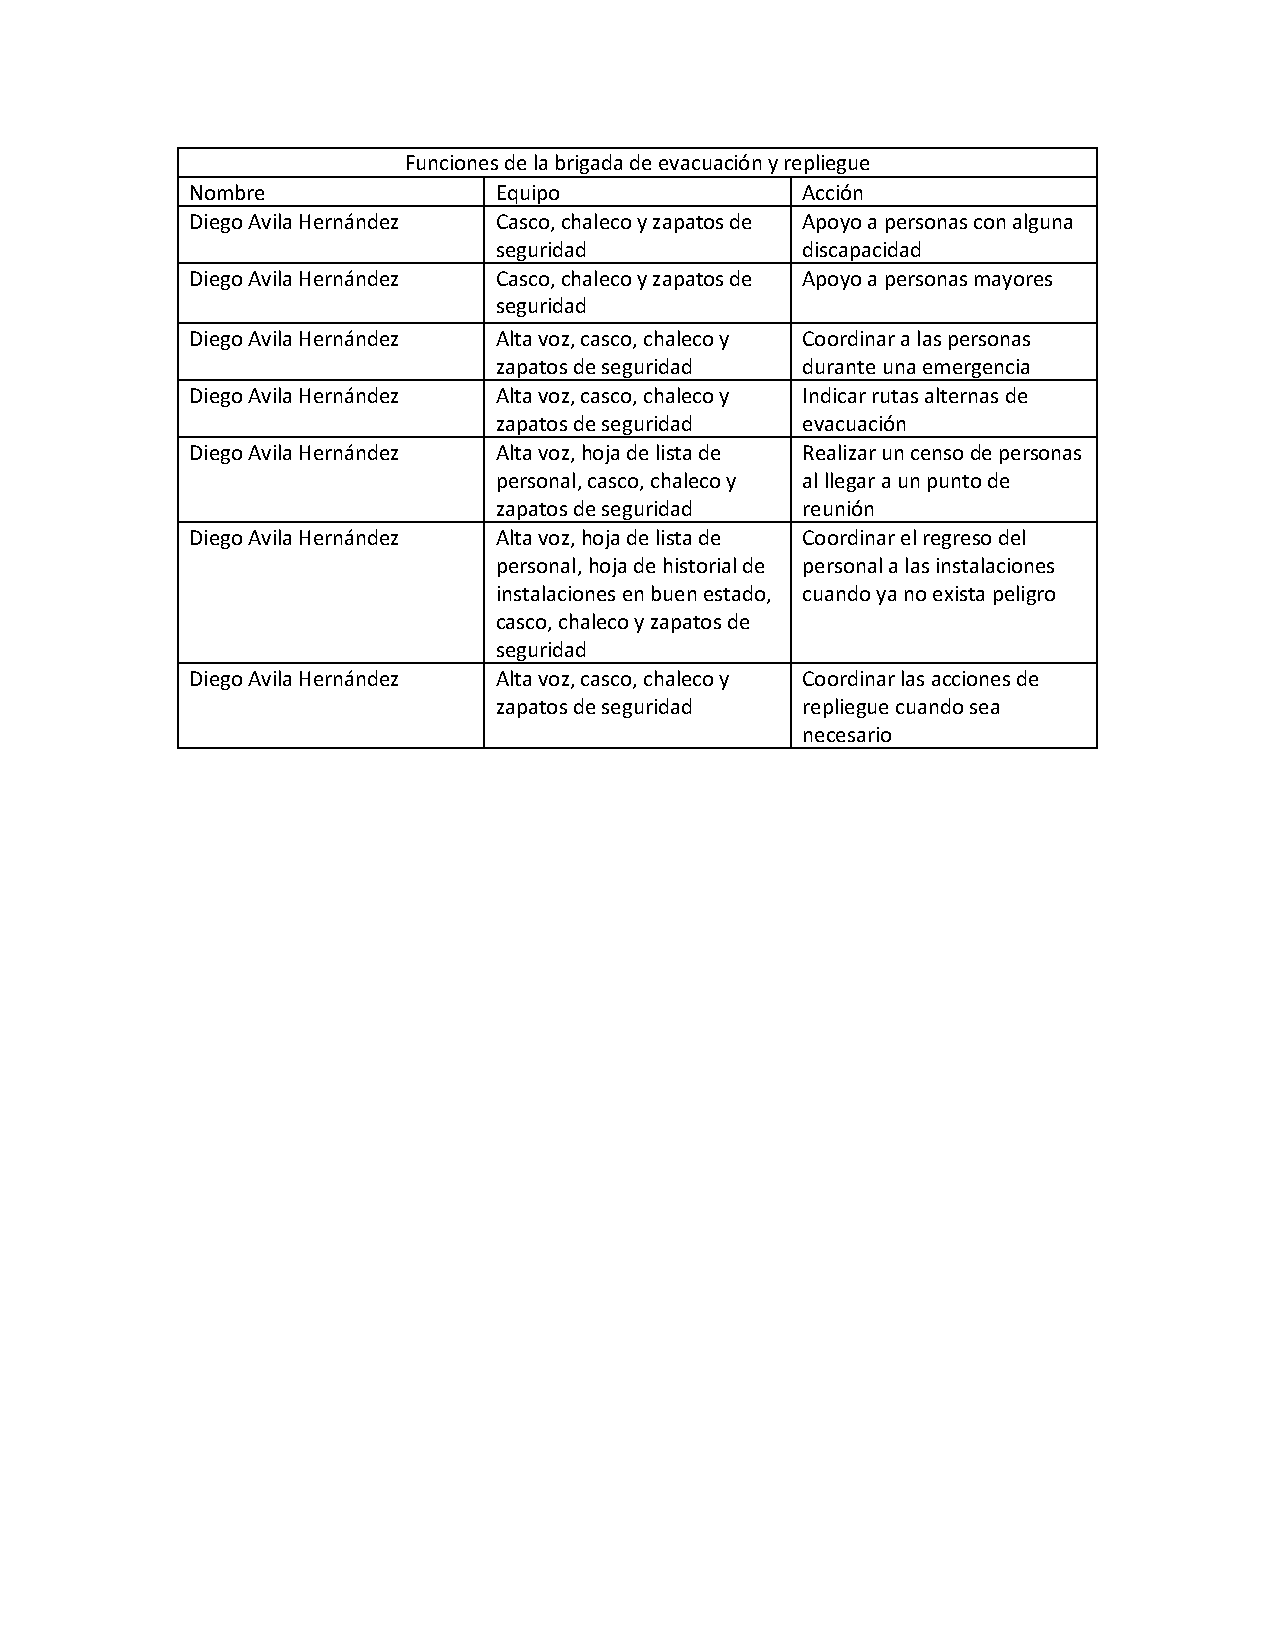
\includegraphics[trim = {20mm 90mm 40mm 45mm},clip,scale=0.5]{22/Img/brigada.pdf}
       % \caption{Acciones asignadas a cada integrante del equipo de trabajo en caso de una evacuación de emergencia o repliegue.}
        %\label{fig:brigada}
    %\end{figure}
    
    
    \subsubsection{Directorio de telefónicos de emergencia}
    
    
    
    \begin{figure}[H] 
        \centering
        \includegraphics[trim = {40mm 52mm 40mm 7mm},clip,scale=0.4]{22/Img/directorioTelefónicoParaEmergencias.pdf}
        \caption{Directorio telefónico de emergencias}
        \label{fig:Directorio}
    \end{figure}
    
    
    
    \subsection{Análisis de los métodos, materiales, herramientas e instalación utilizada en la ejecución del ensamble de un circuito electrónico}
    
    \subsubsection{Verificación}
    
    Costos de no calidad.
    % 
    % 
    \subsubsection{Desarrollo del sistema de tiempos predeterminado}
    % 
    % 
    \subsubsection{Desarrollo del muestreo del trabajo}
    % 
    %
    En el desarrollo del proyecto se planteó el problema de la fata de datos como lo son la media y la varianza de nuestra población, los cuales en nuestro análisis forman una parte fundamental para llegar a nuestros resultados. 
    
     \begin{equation}
            \label{equ:media}
           \mu = \dfrac{b+a}{2}
        \end{equation}
    
      \begin{equation}
            \label{equ:des}
            \sigma = \sqrt{\dfrac{(b-a+1)^2-1}{12}}
        \end{equation}
    
    
    
    Para ello se implementó varios métodos, uno de ellos es con el uso de las probabilidades, en donde para obtener la media poblacional se usó la ecuación \ref{equ:media} y para  la desviación estándar utilizamos la ecuación \ref{equ:des}, donde estás fórmulas nos ayudan a estimar la tendencia central de nuestra población con tan solo dos muestras, reduciendo así el costo de información y tiempo. Por esto mismo se logra fundamentar el porqué de la cantidad de observaciones que se realizaron en este proyecto, las cuales fueron dos, ya que solo es necesario estos dos valores para utilizar la ecuación \ref{equ:media}.
       
    \begin{figure}[H]
        \centering
        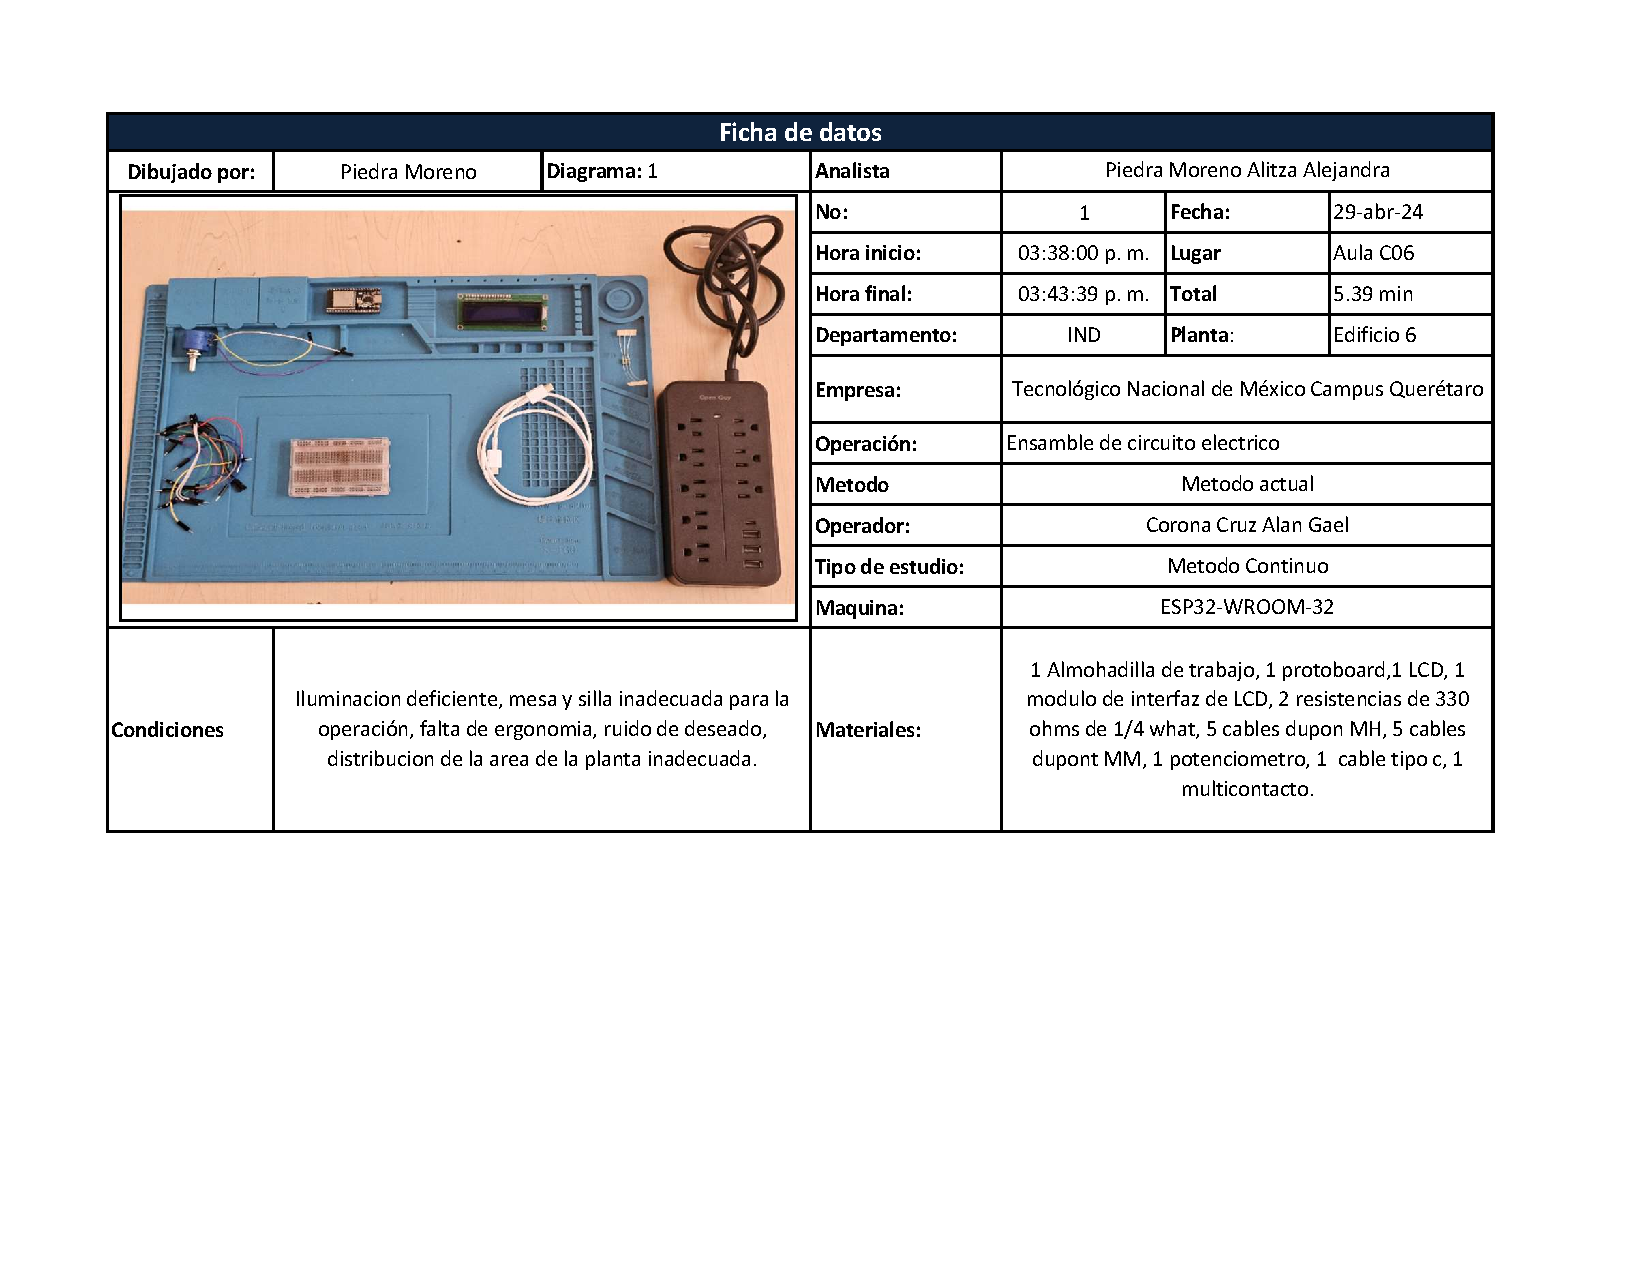
\includegraphics[trim = {17mm 70mm 25mm 15mm},clip,scale=0.37]{22/Img/hojaDeDatos1.pdf}
        \caption{Hoja de datos de la primera observación}
        \label{fig:hoja1}
    \end{figure}
    
    
    Para determinar el tiempo ciclo se generó un método de muestreo en el cual para ello se utilizó el método probabilístico, por lo cual sé generaron dos muestras en distintos momentos, dado que son variables mutuamente excluyentes, y dado que nuestro objetivo es encontrar una muestra que describa de forma precisa nuestro valor real. En la tabla mostrada en la figura \ref{fig:hoja1} se colocaron los datos más fundamentales e indispensable para el desarrollo de nuestro análisis, con estos datos registrados podemos empezar a analizar las imágenes pertinentes a la evidencia de la primera muestra, la cual fue tomada el día 29 de abril en el aula C06. Como de muestra en la figura \ref{fig:evi0} se presenta la imagen capturada del operador iniciando la operación con la distribución definida anteriormente, igual podemos observar un poco de las condiciones en las que se encuentran trabajando. 
    
    
    
    De igual forma, en la figura \ref{fig:evi1} podemos observar el momento en  el que el operador está conectando el potenciómetro en el protoboard, como se puede observar en la imagen el operador está colocando el cable con ambas manos, provocando un movimiento ineficiente dado que el operador podría utilizar ese movimiento para realizar otra operación.
    
    
    \begin{figure}[H]
        \centering
        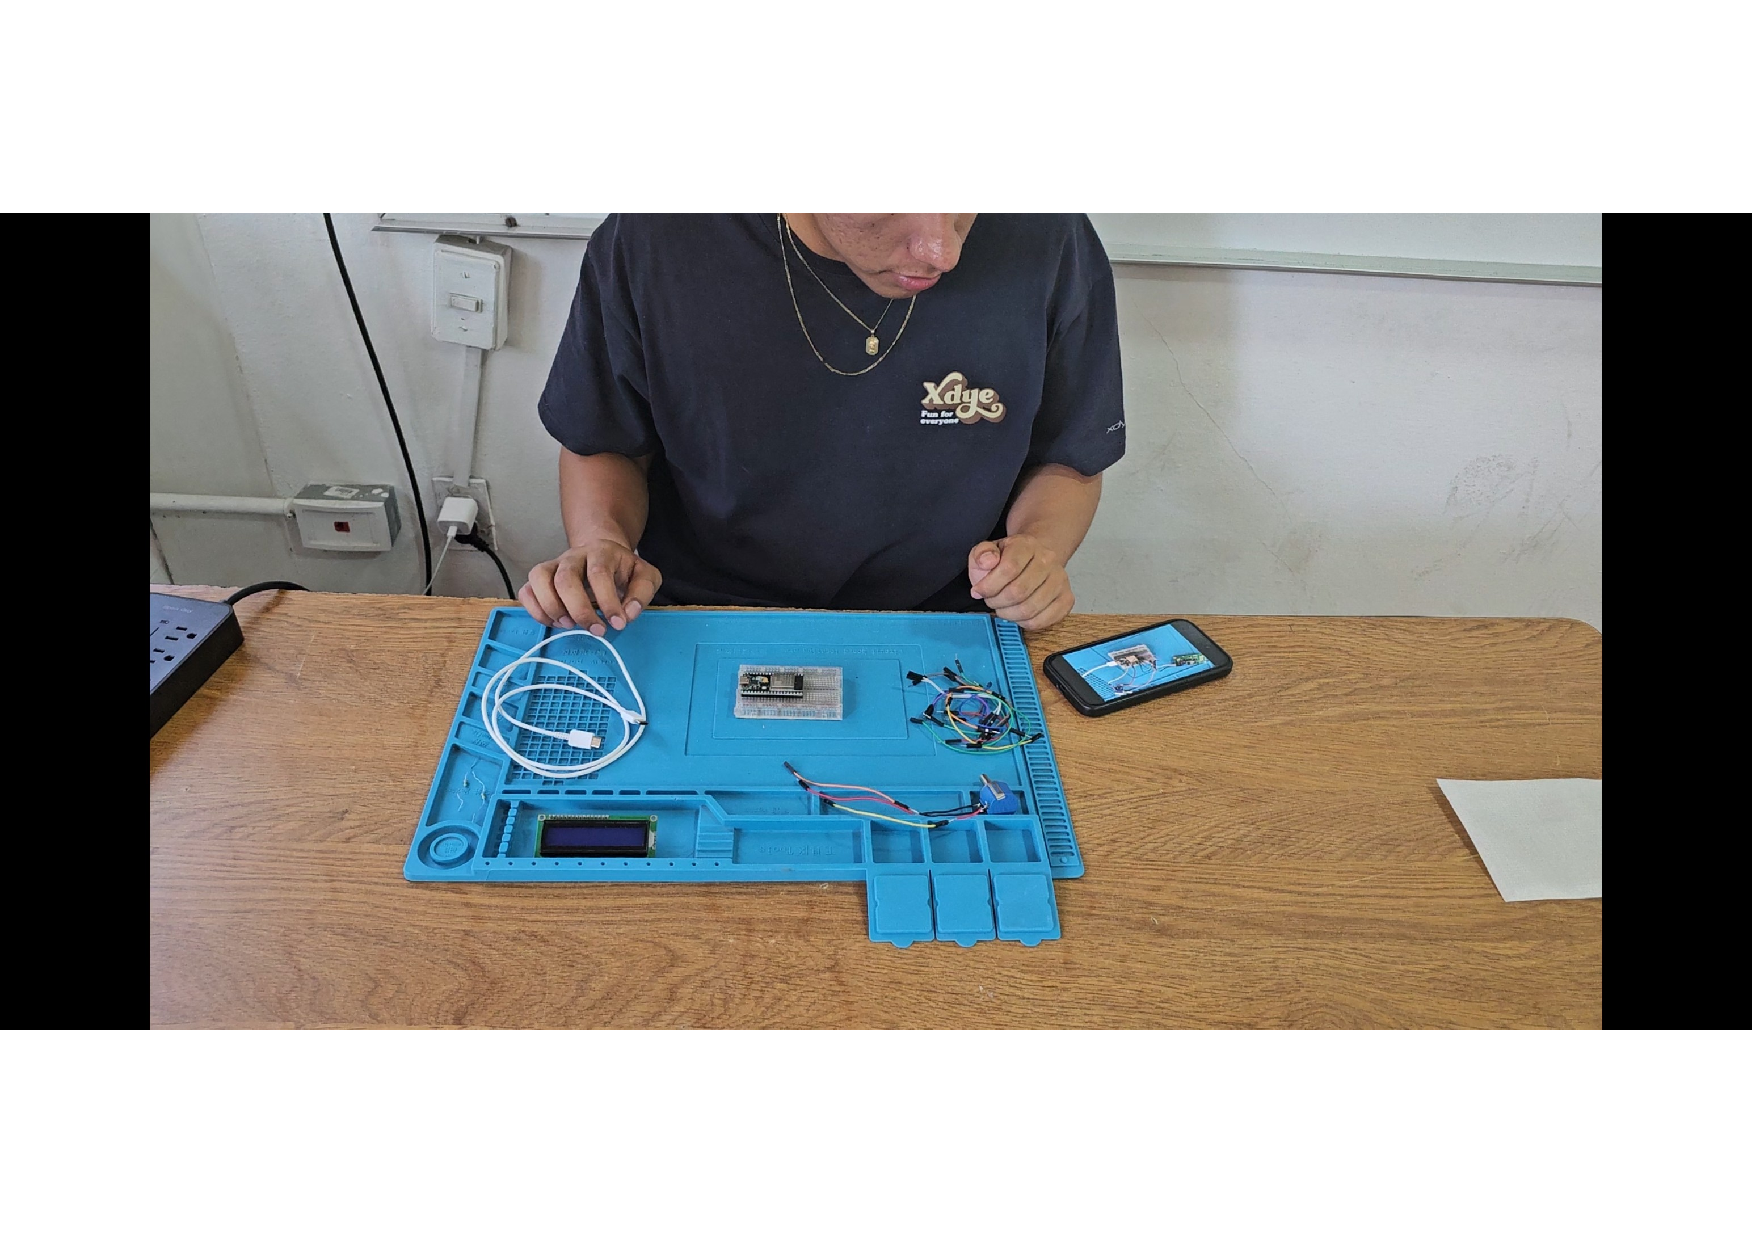
\includegraphics[trim = {25mm 40mm 25mm 10mm},clip,scale=0.3]{22/Img/e1.pdf}
        \caption{Inicio de la operación}
        \label{fig:evi0}
    \end{figure}
    
    
    
    Por otra parte, en la figura \ref{fig:evi2} se enseña como el operador lleva desarrollando el ensamble ya con un avance significativo, posterior a esto en la figura \ref{fig:evi3} está colocando la LCD, aunque ciertamente este paso iba antes, y por ello mismo se observa en el video como el operador batalla para colocar las resistencias por el cable que las atraviesan y por ende este paso se complica un poco más, y esto a su vez puede conducir a una perdida de tiempo así como generar una mala conexión lo cual solo podría causar consecuencias negativas, por ello la importancia de una buena planeación a la hora de desarrollar el manual así como la capacitación del operador con los métodos, para su aprendizaje adecuado.
    
    
       
    \begin{figure}[H]
        \centering
        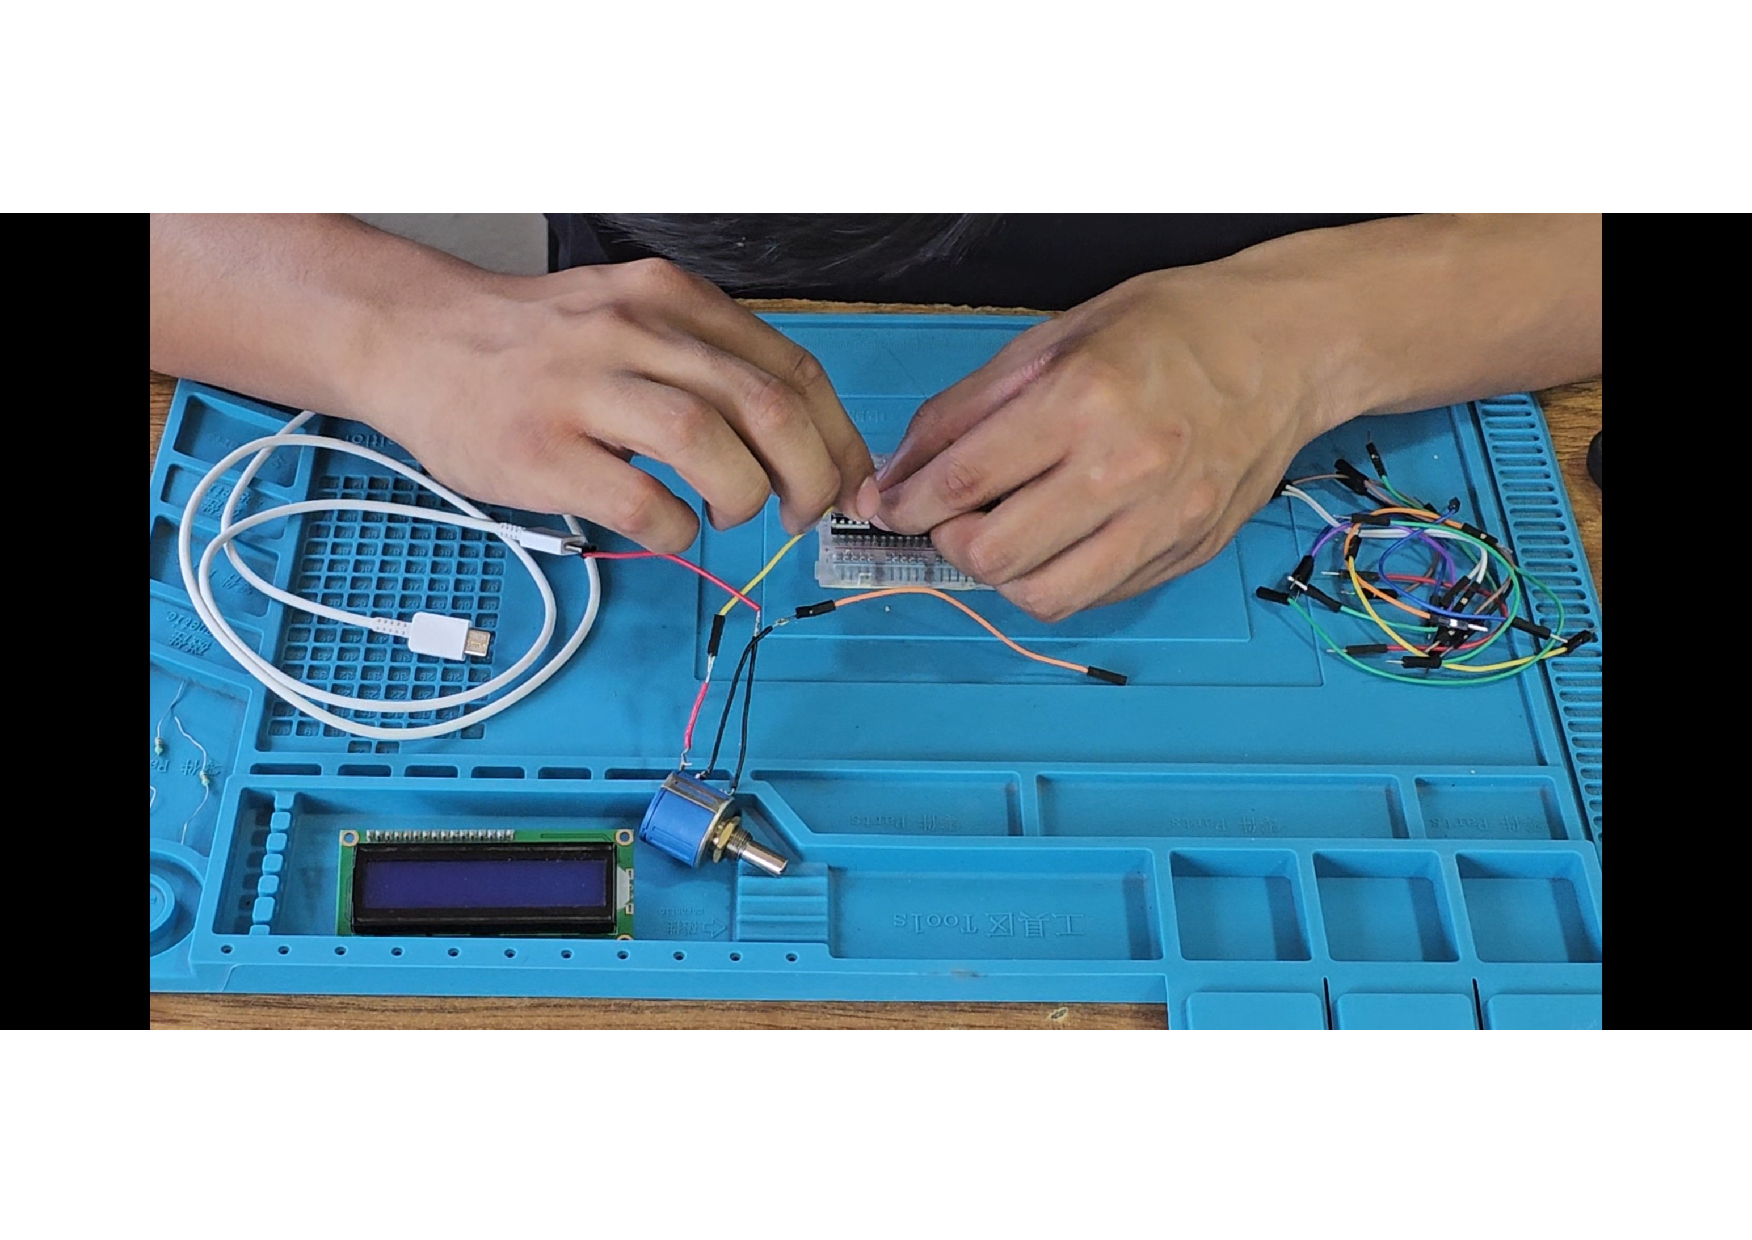
\includegraphics[trim = {25mm 25mm 25mm 10mm},clip,scale=0.3]{22/Img/e2.pdf}
        \caption{Ensamble del potenciómetro}
        \label{fig:evi1}
    \end{figure}
    
    
    
     Así mismo en la figura \ref{fig:evi4} observamos como el operador procede a conectar la ESP32 a la fuente de energía y en ese momento como se observa en la figura \ref{fig:evi5} empieza a encender la LCD y trata unos cuantos segundos en aparecer el texto, posterior a esto el operador voltea la LCD para observar los datos e interactuar con los valores del potenciómetro como se observa en la figura \ref{fig:evi6} en la cual el operador está agarrando el potenciómetro con una mano y la otra mueve el interruptor o cursor de este, ya por último en la figura \ref{fig:evi7} sé amplio la imagen para ver la pantalla de la LCD  ya que no es muy visible en la figura anterior.
    
     \begin{figure}[H]
        \centering
        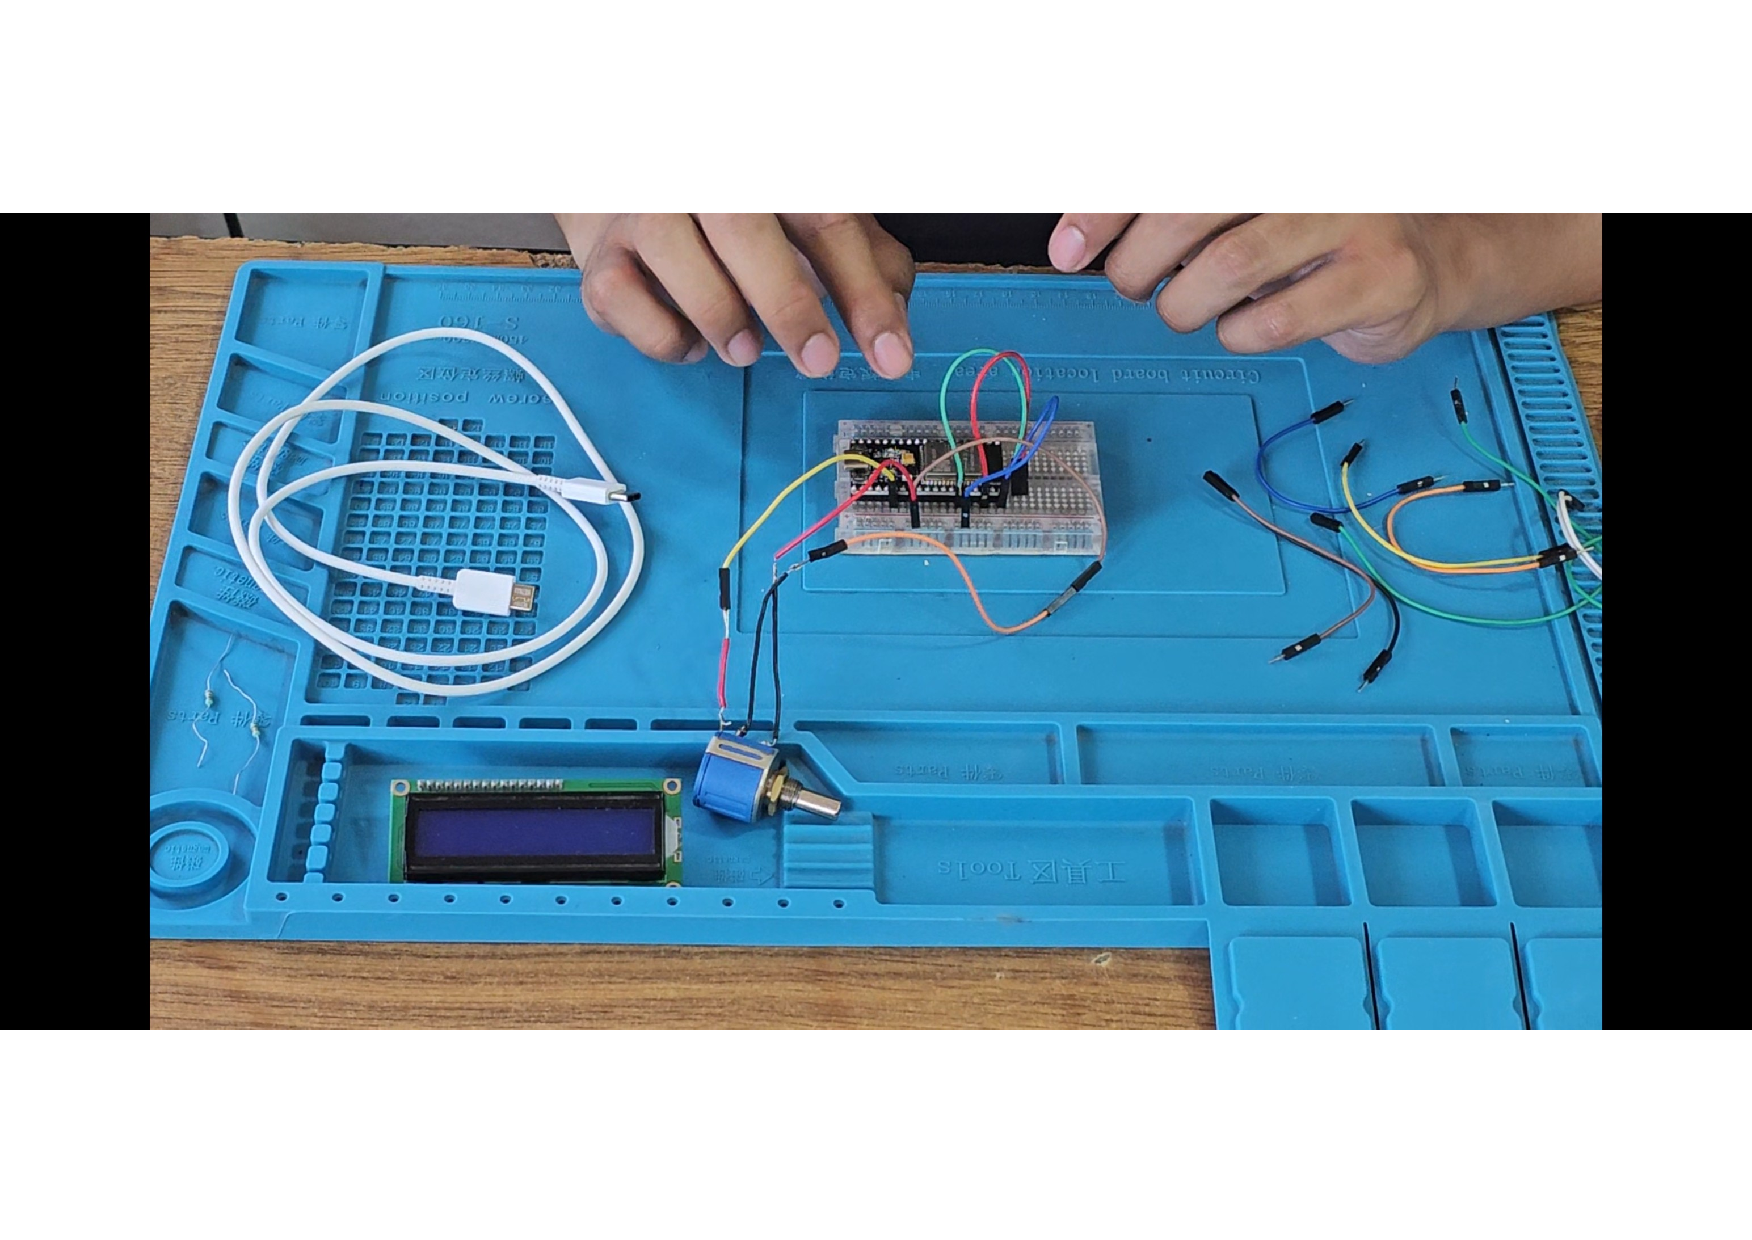
\includegraphics[trim =  {25mm 25mm 25mm 10mm},clip,scale=0.3]{22/Img/e5.pdf}
        \caption{Operación a mitad de la secuencia}
        \label{fig:evi2}
    \end{figure}
    
    
    \begin{figure}[H]
        \centering
        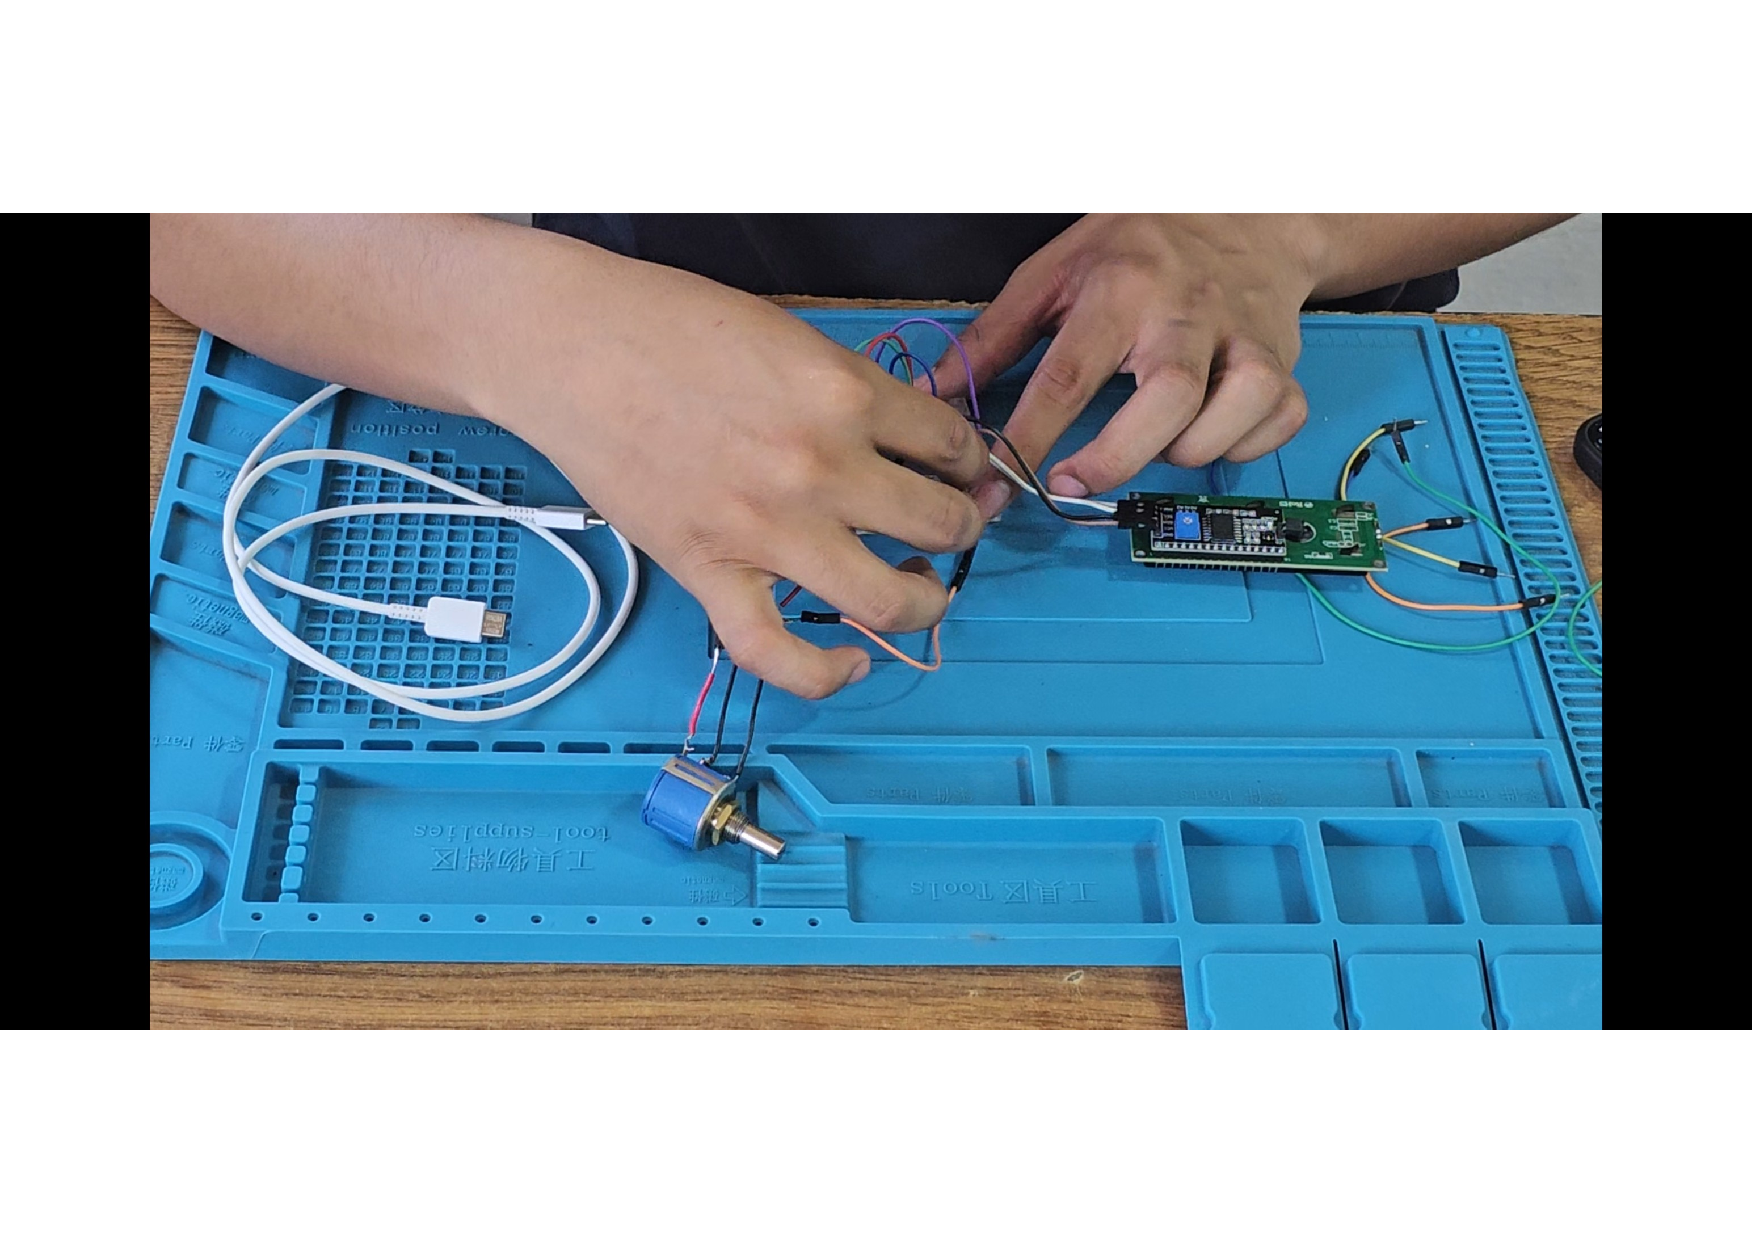
\includegraphics[trim =  {25mm 25mm 25mm 10mm},clip,scale=0.3]{22/Img/e8.pdf}
        \caption{Colocación de la LCD}
        \label{fig:evi3}
    \end{figure}
    
    
    \begin{figure}[H]
        \centering
        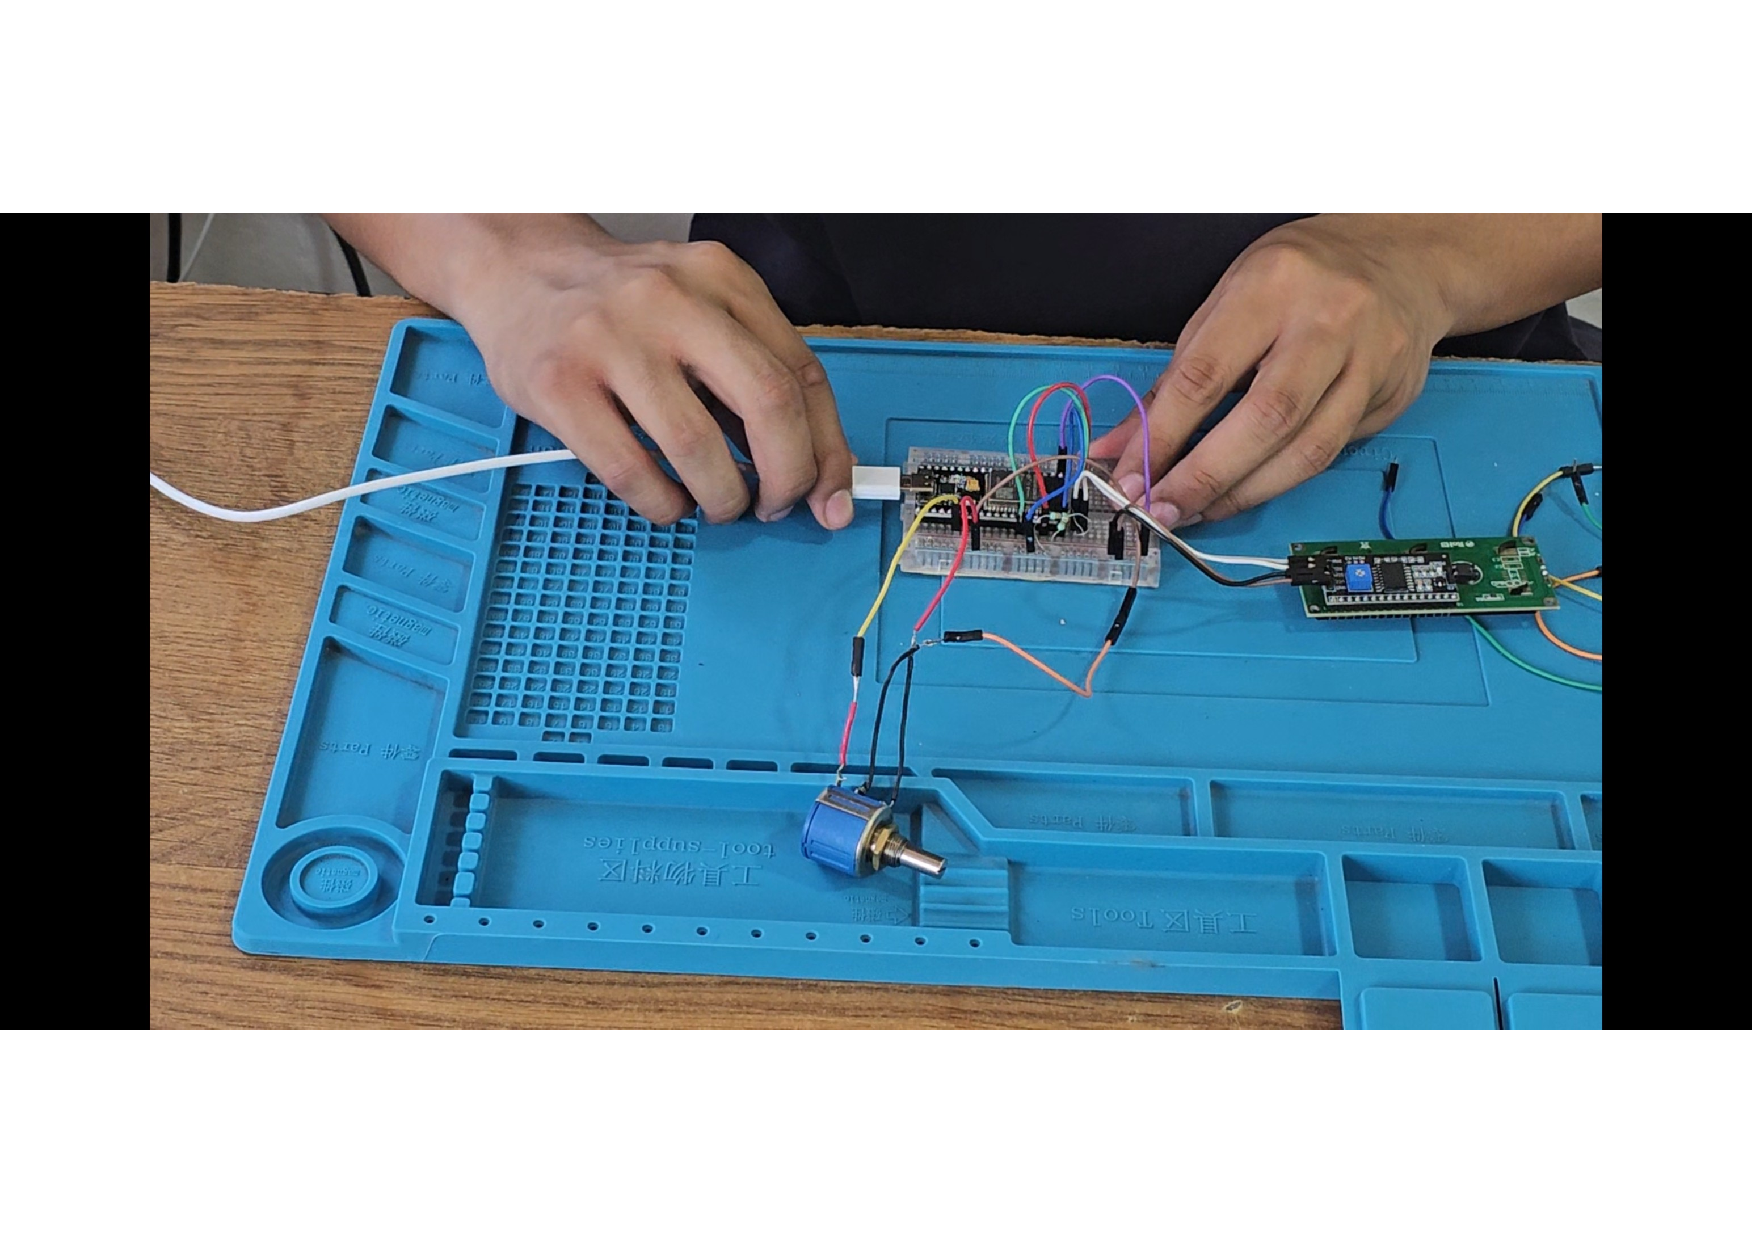
\includegraphics[trim = {25mm 25mm 25mm 10mm},clip,scale=0.3]{22/Img/e10.pdf}
        \caption{Conexión al cable C}
        \label{fig:evi4}
    \end{figure}
    
    
    \begin{figure}[H]
        \centering
        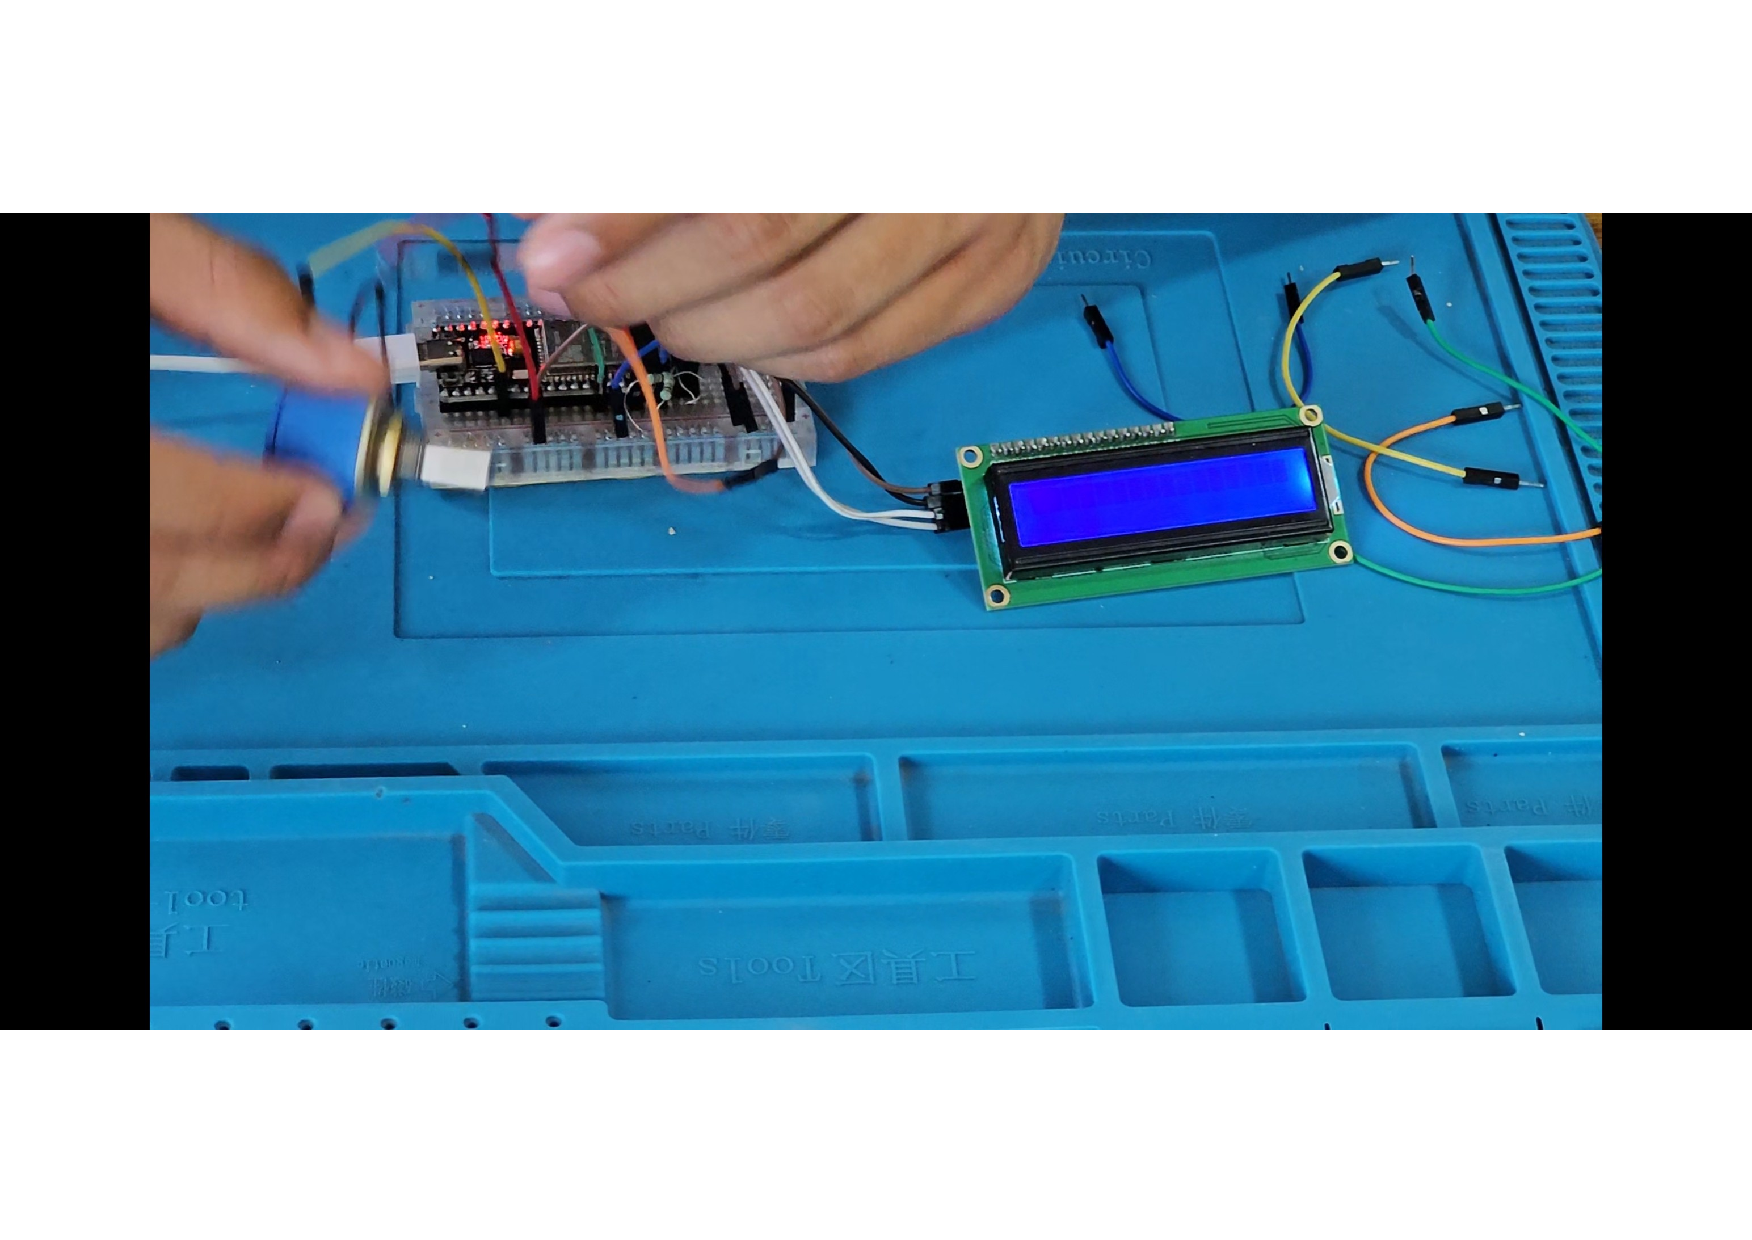
\includegraphics[trim =  {25mm 25mm 25mm 10mm},clip,scale=0.3]{22/Img/e12.pdf}
        \caption{Proceso de encendido de la LCD}
        \label{fig:evi5}
    \end{figure}
    
    
    \begin{figure}[H]
        \centering
        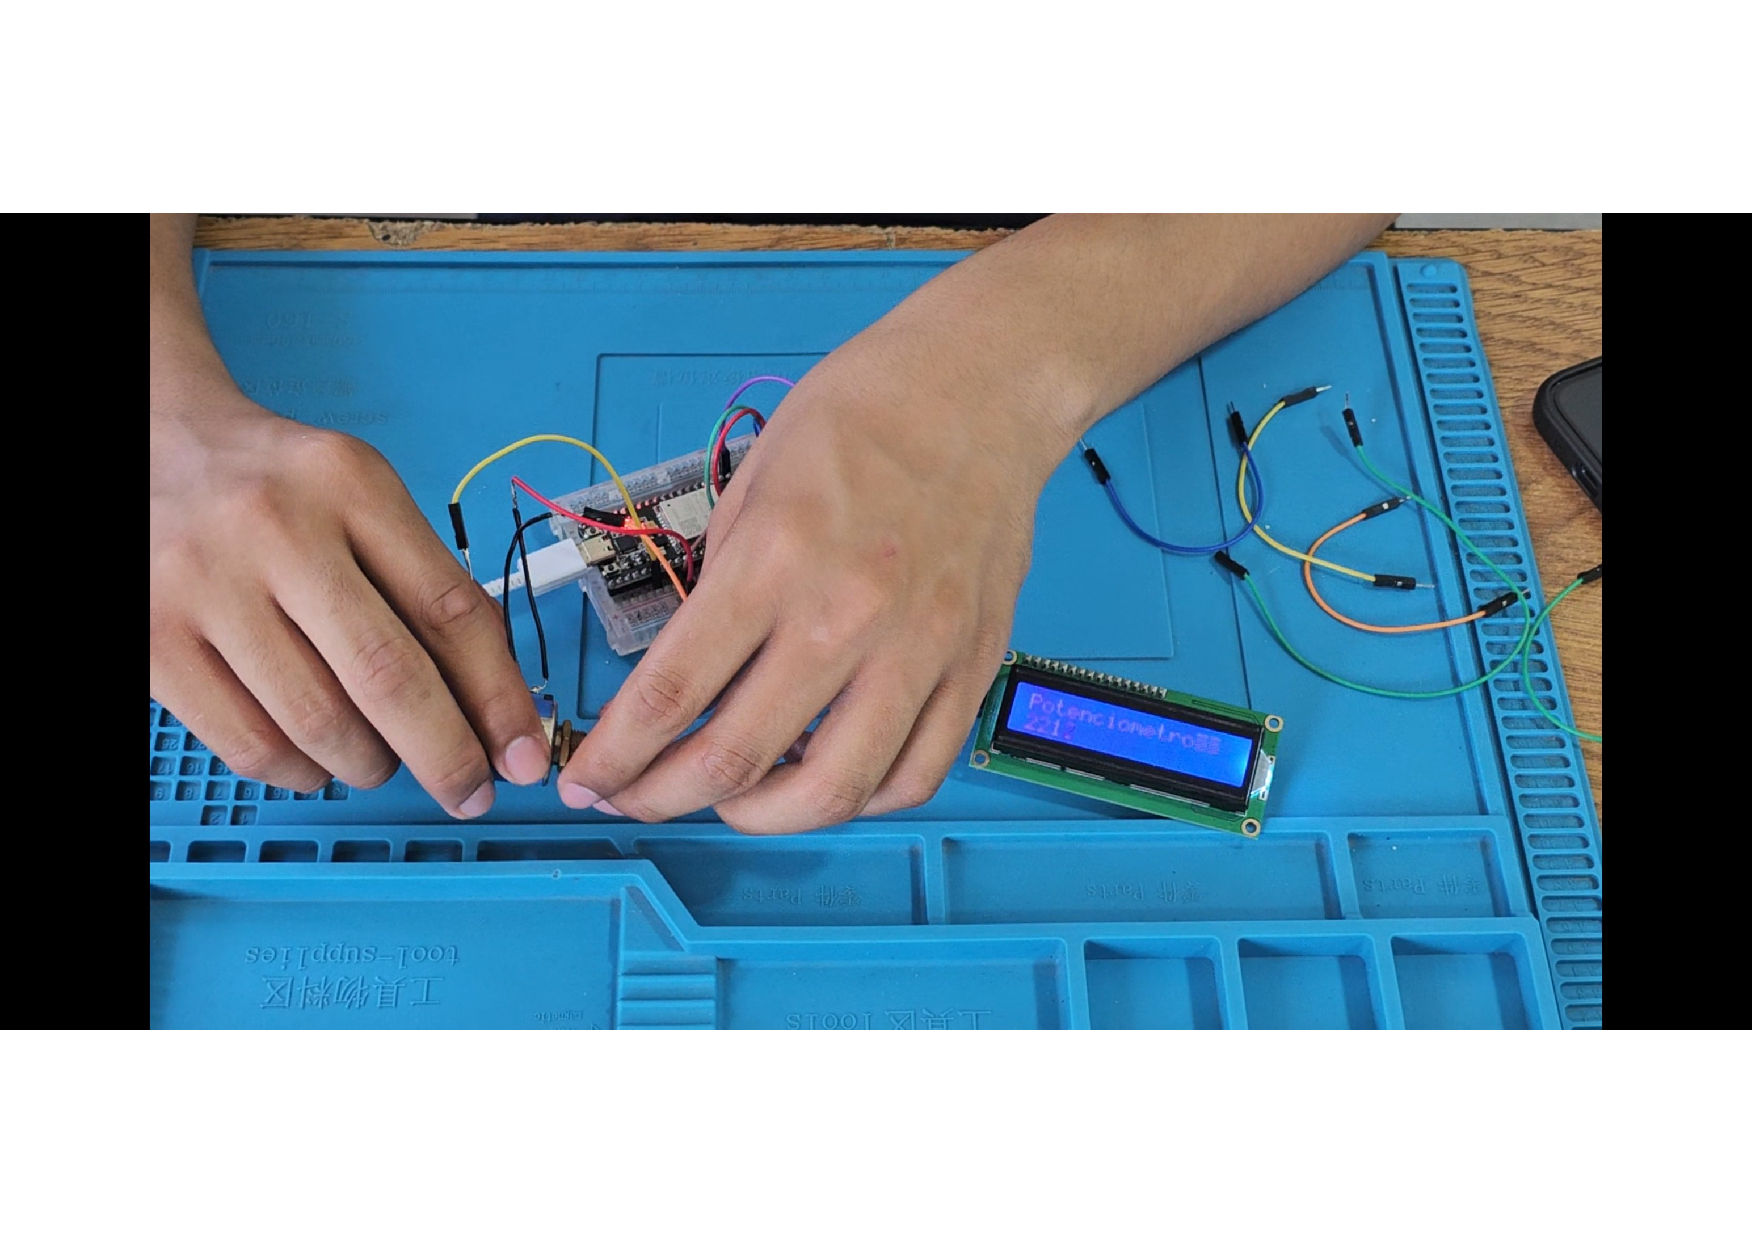
\includegraphics[trim = {25mm 25mm 25mm 10mm},clip,scale=0.3]{22/Img/e15.pdf}
        \caption{Interacción con el potenciómetro}
        \label{fig:evi6}
    \end{figure}
    
    
    \begin{figure}[H]
        \centering
        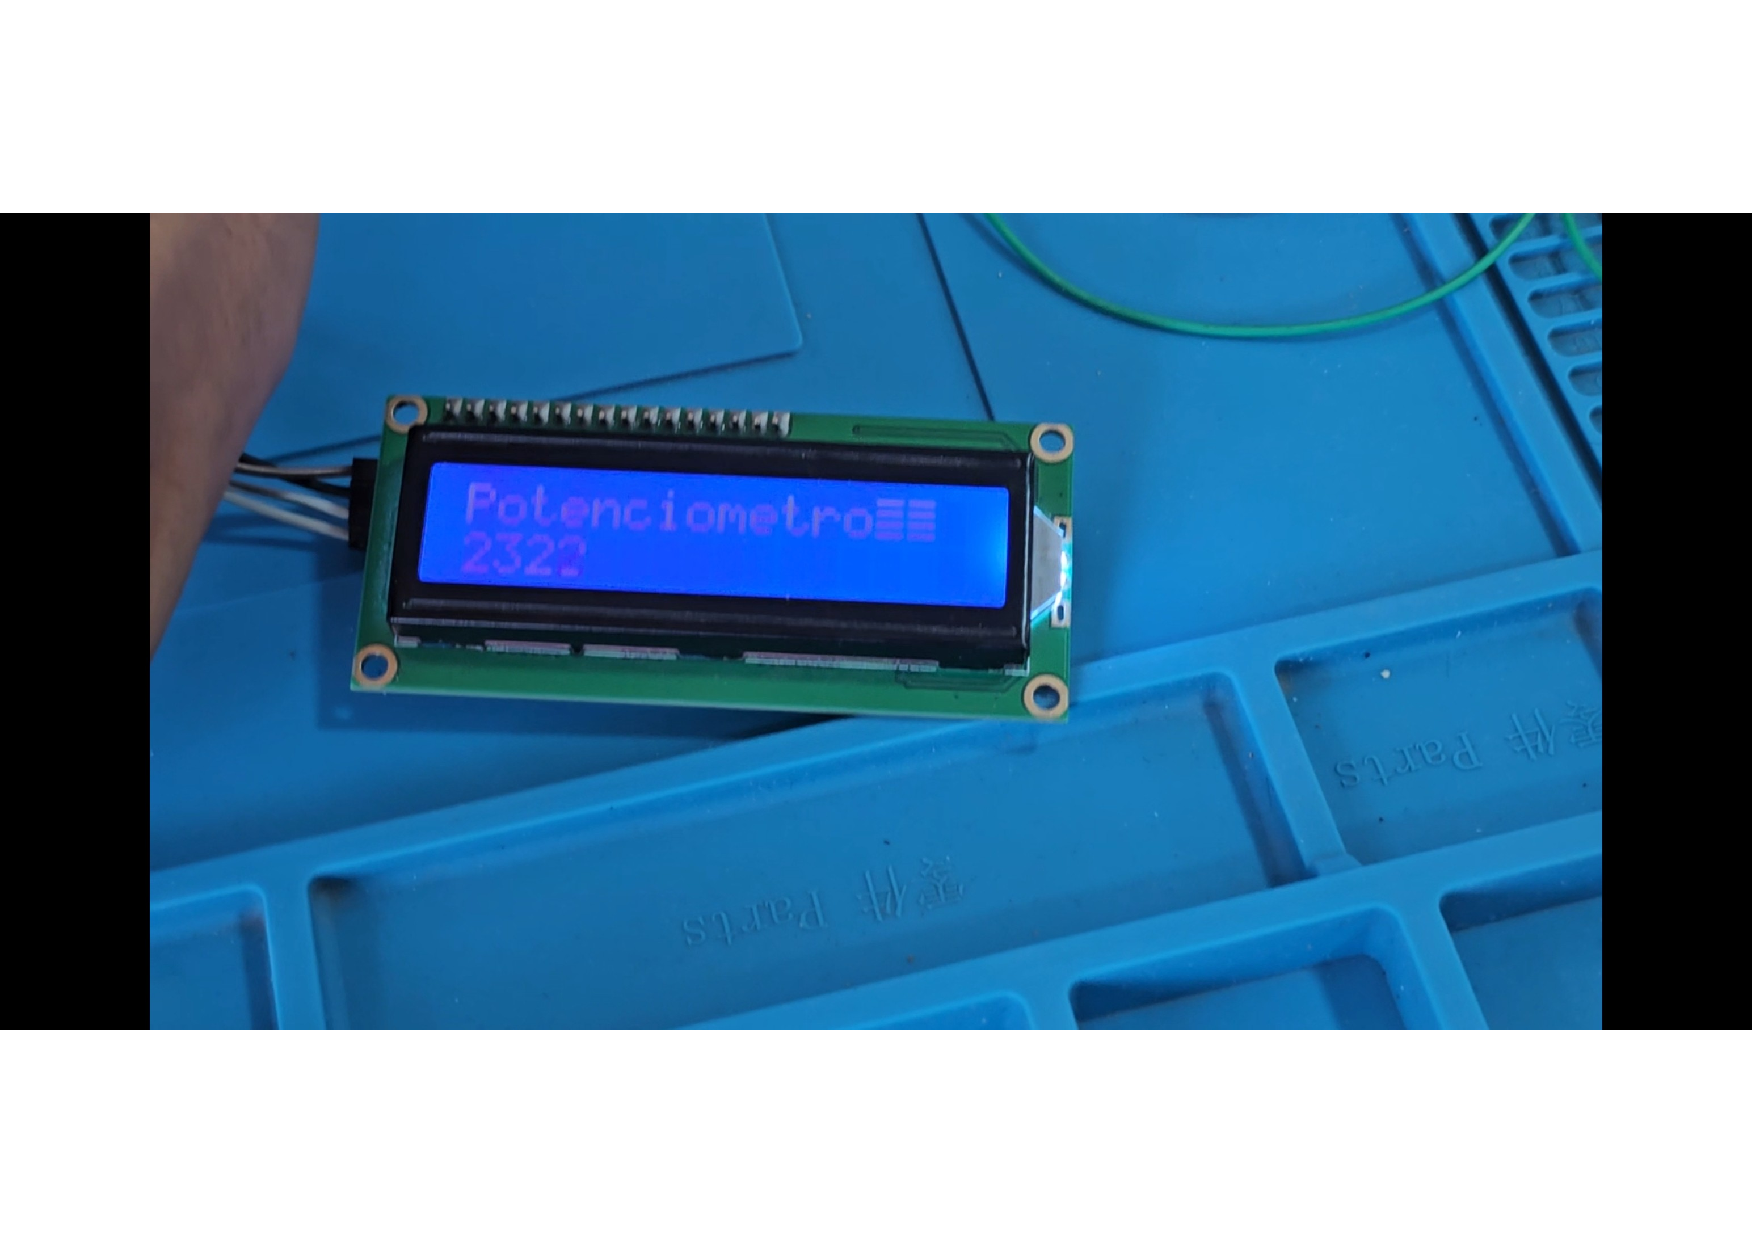
\includegraphics[trim =  {25mm 25mm 25mm 10mm},clip,scale=0.3]{22/Img/e17.pdf}
        \caption{Encuadre de la LCD}
        \label{fig:evi7}
    \end{figure}
    
    
    \begin{figure}[H]
        \centering
        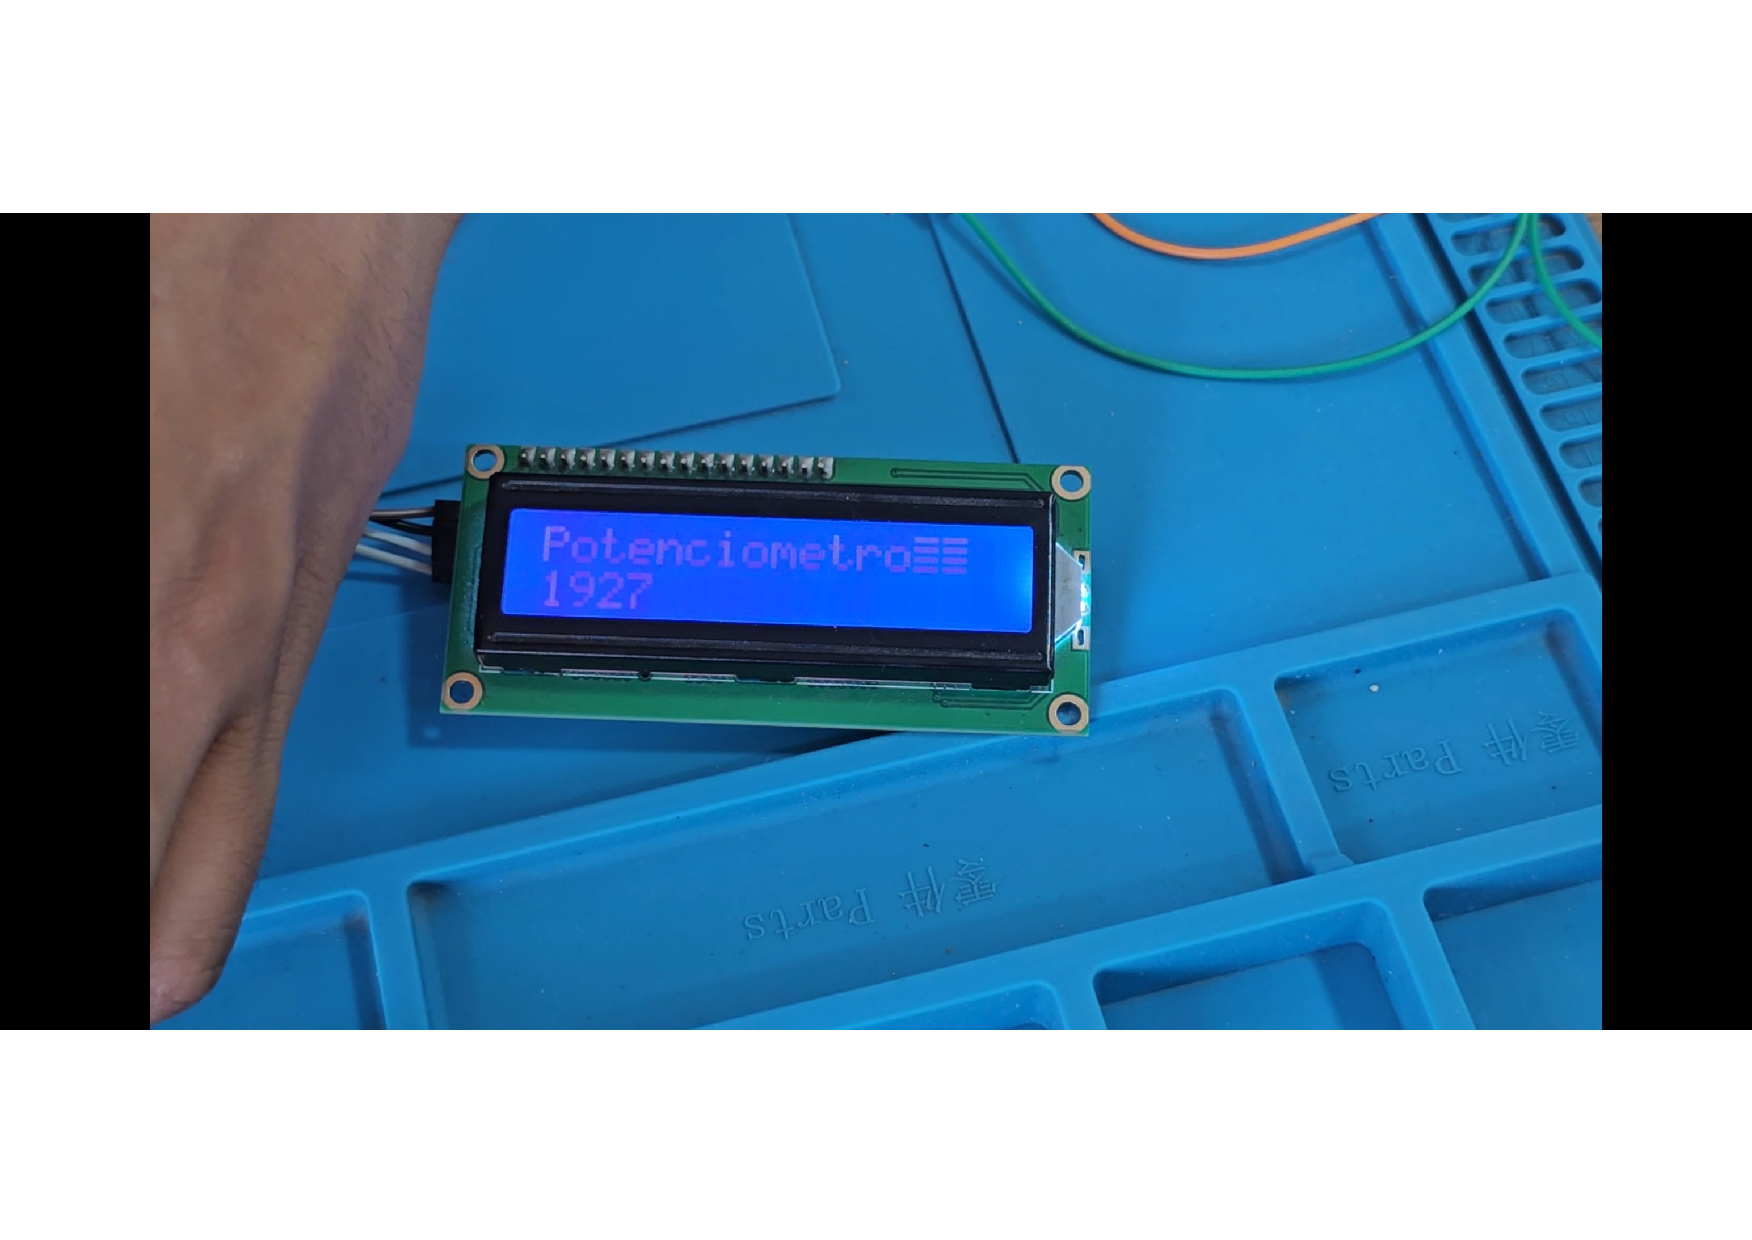
\includegraphics[trim =  {25mm 25mm 25mm 10mm},clip,scale=0.3]{22/Img/e20.pdf}
        \caption{Cambio de valor}
        \label{fig:evi8}
    \end{figure}
    
    Posterior a recolectar esta muestra de datos, se realizó otro muestreo 3 días después, para ello de igual forma se registraron los datos pertinentes en la tabla mostrada en la figura \ref{fig:hoja2}, de igual forma solo se registraron los datos esenciales para nuestro análisis.
    
    
     Con estos datos a la mano se puede empezar el análisis pertinente y muestreo de nuestra operación, para empezar, en la figura \ref{fig:ev1} se observa como el operador comienza con el ensamble, de antemano se apoyó del instructivo para evitar equivocaciones, con esto mencionado el operador tomo el potenciómetro, conecto el cable con una mano a la ESP y con la otra sostuvo el proto lo cual puede causar un movimiento ineficiente, ya que para ser más rápido, el operador pudo conectar dos cables al mismo tiempo.
    
    \begin{figure}[H]
        \centering
        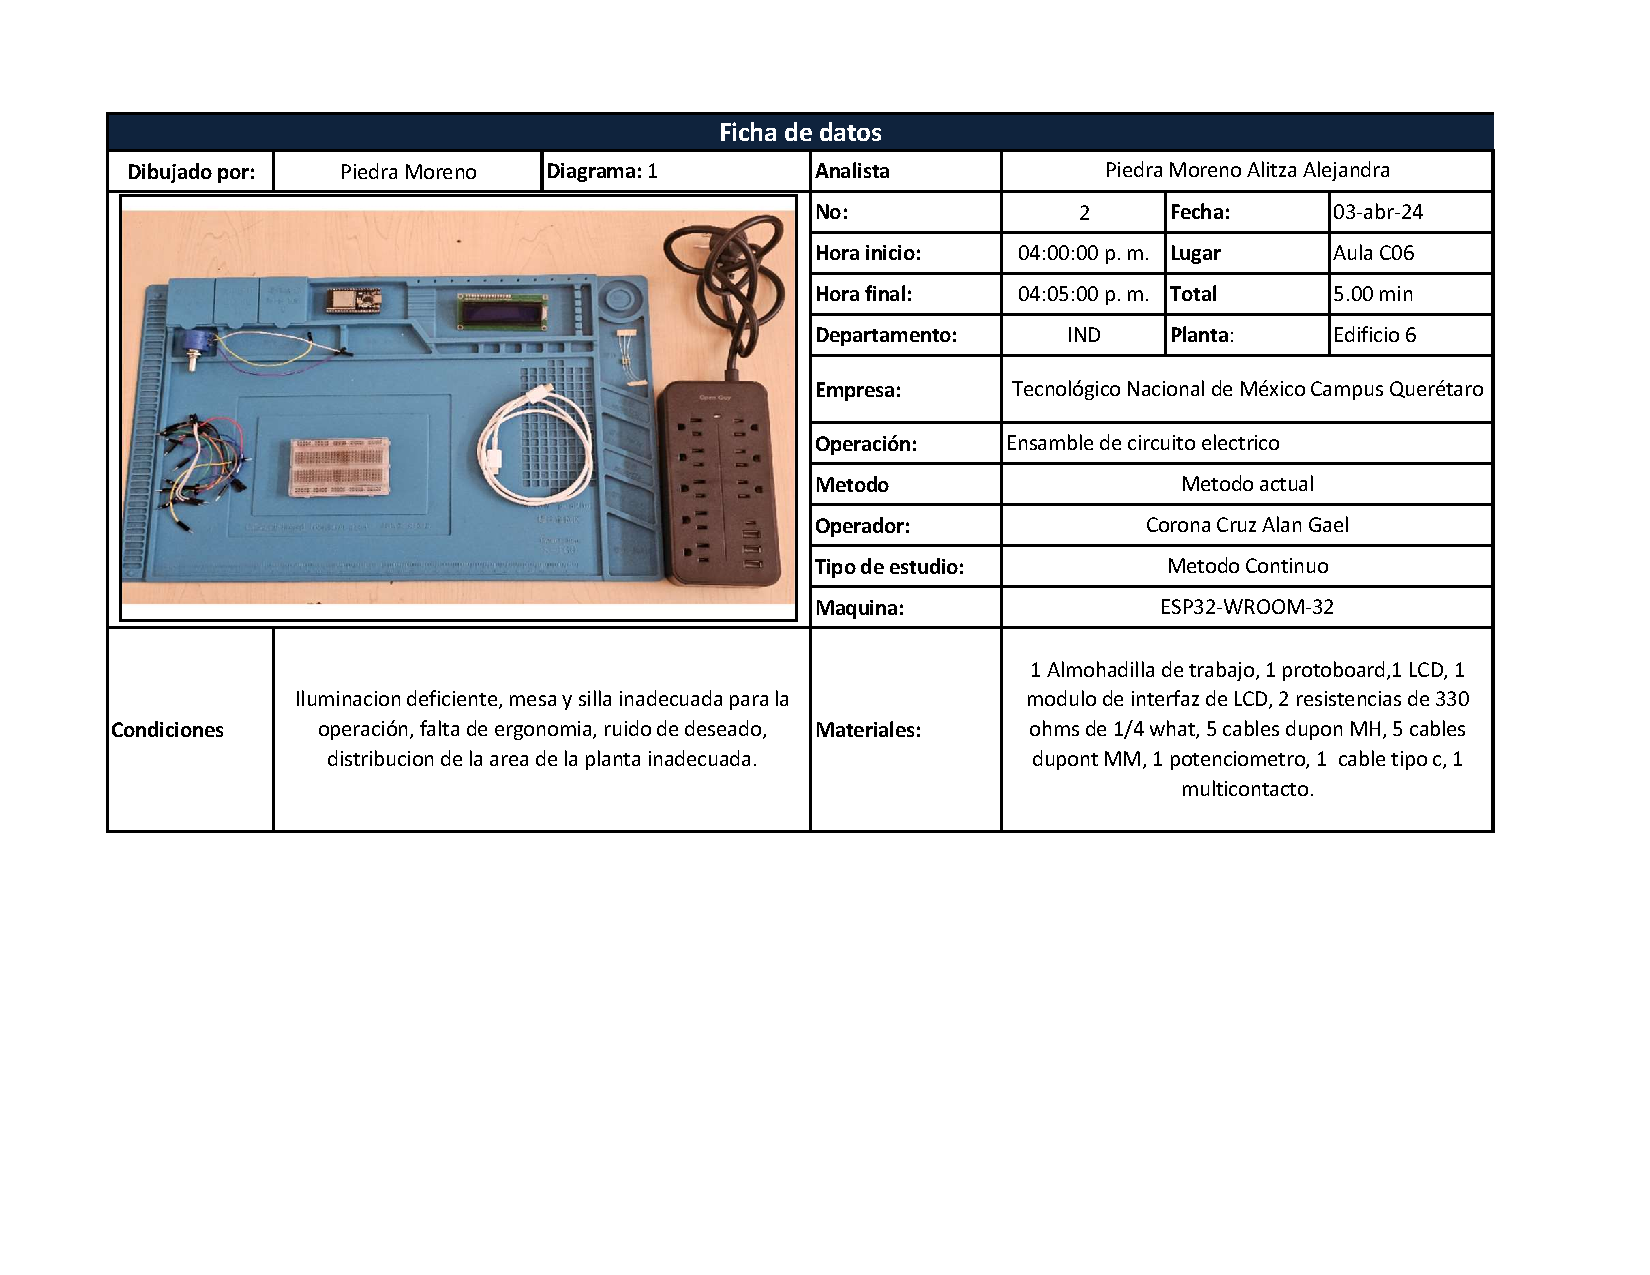
\includegraphics[trim = {17mm 70mm 25mm 15mm},clip,scale=0.37]{22/Img/hojaDeDatos2.pdf}
        \caption{Hoja de datos para la segunda muestra}
        \label{fig:hoja2}
    \end{figure}
    
     
     Por otra parte, en la figura \ref{fig:evi2} se observa al operador conectar la LCD, en esta observamos como el operador conecta con una mano y con la otra mano sostiene, pero como se guio con el instructivo podemos cambiarlo para que conecte los dos cables al mismo tiempo, ya que este puede ayudarnos a reducir tiempos o de igual forma generar mayor comodidad a la hora de realizar la operación, ya para la figura \ref{fig:evi3} se observa  al operador conectar los últimos cables para el buen funcionamiento de nuestro circuito, así mismo en la figura \ref{fig:evi4} el operador conecta la ESP al cable tipo C y a la energía, esto para probar el funcionamiento del circuito, posterior a esto se observa la interacción del operador con el potenciómetro, y como es que funciona la LCD, igualmente en la figura \ref{fig:evi5} se observa un acercamiento a la pantalla del LCD y es una evidencia de que se están enviando correctamente los valores del potenciómetro.
    
     
    \begin{figure}[H]
        \centering
        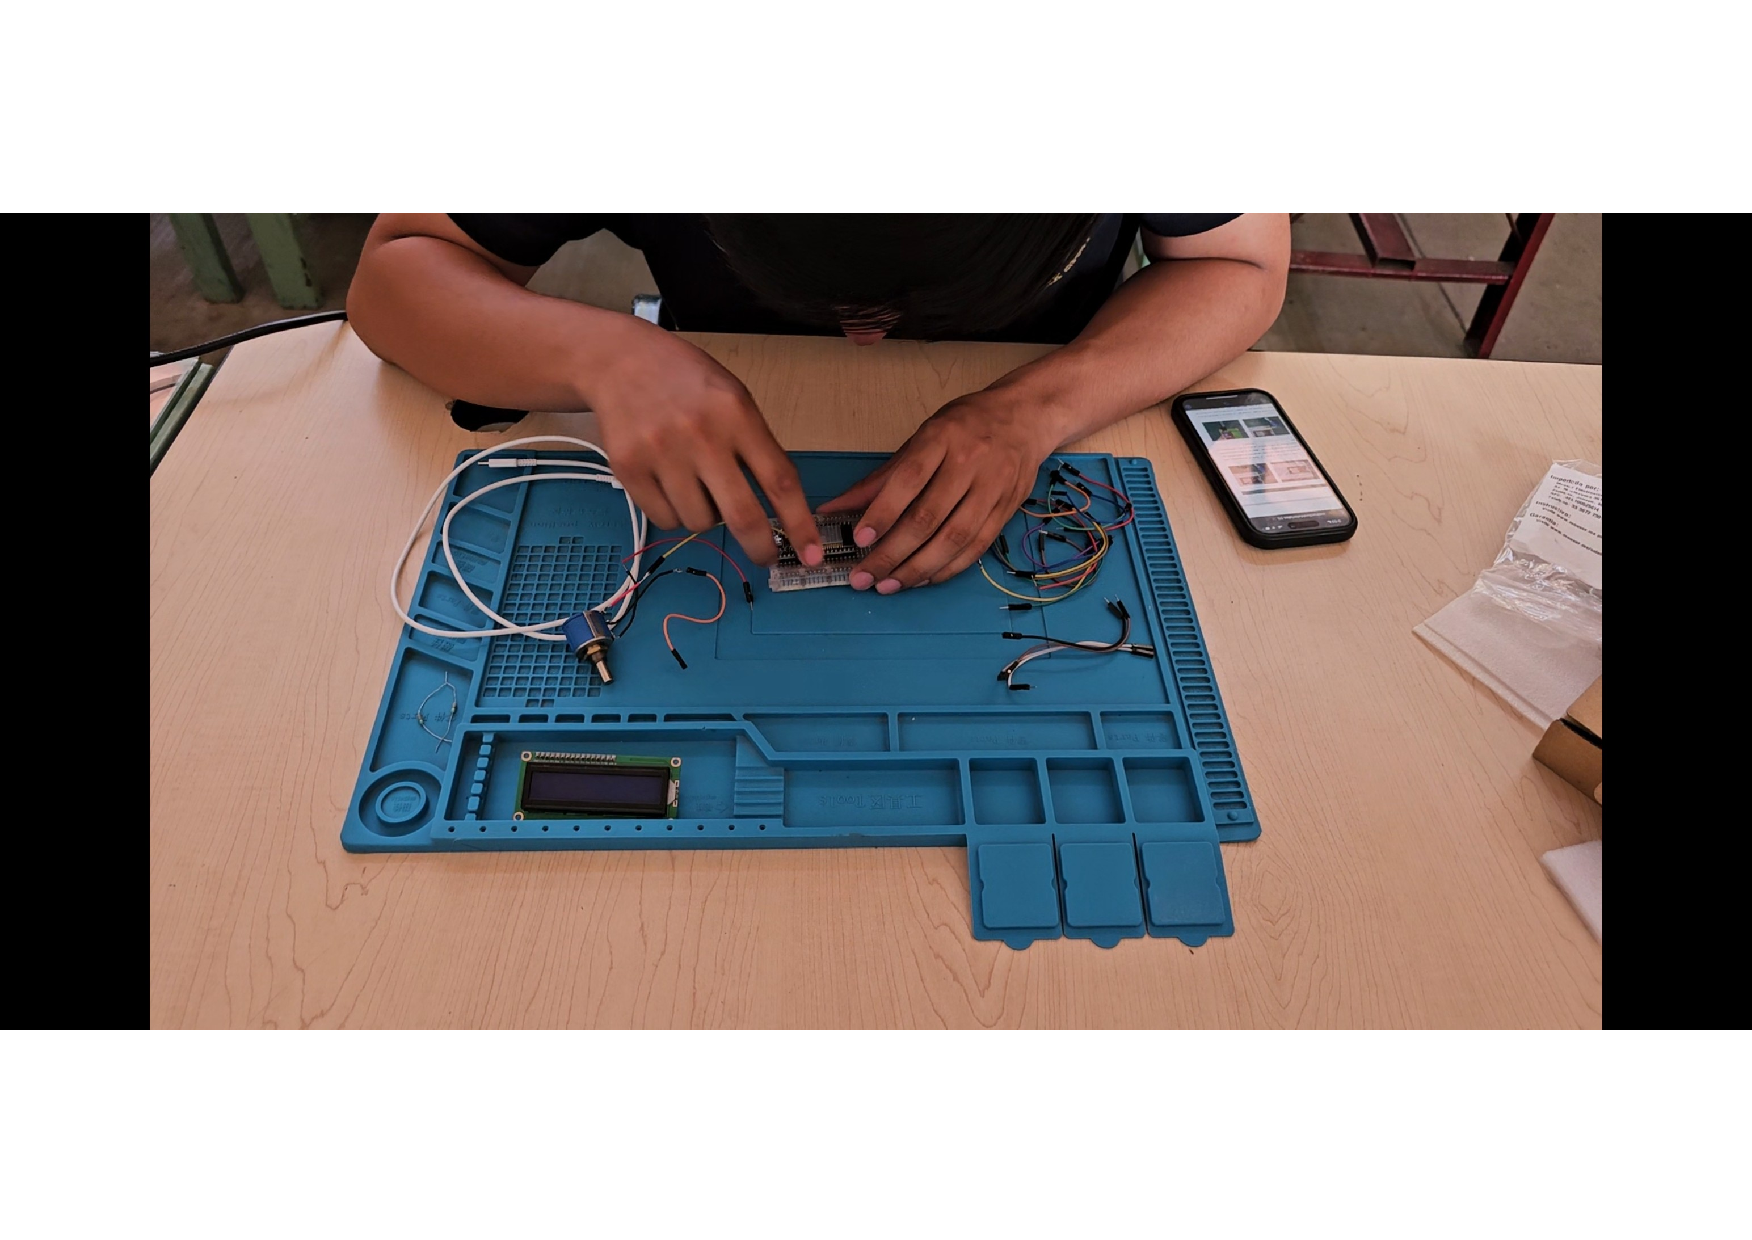
\includegraphics[trim = {25mm 25mm 25mm 10mm},clip,scale=0.3]{22/Img/ev1.pdf}
        \caption{Inicio del ensamble de la muestra 2}
        \label{fig:ev1}
    \end{figure}
    
    \begin{figure}[H]
        \centering
        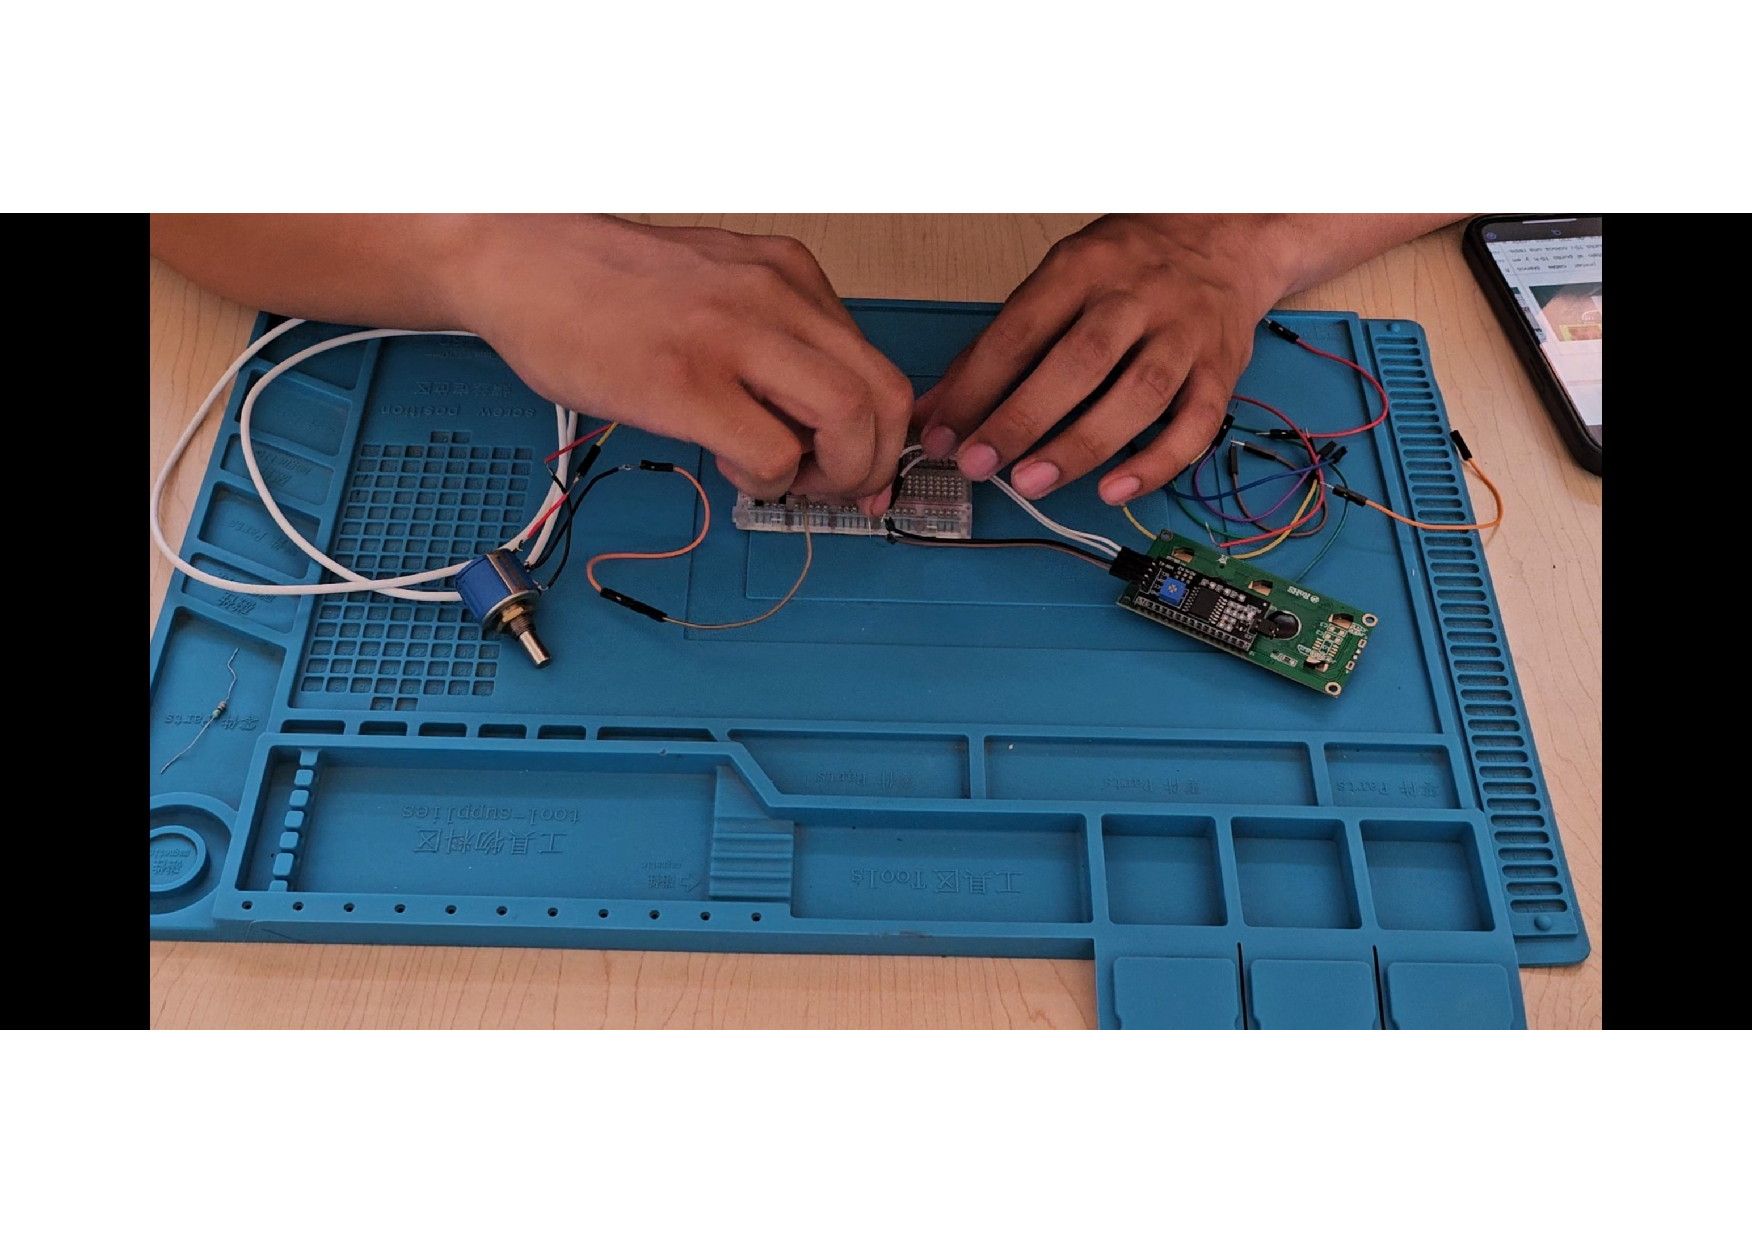
\includegraphics[trim = {25mm 25mm 25mm 10mm},clip,scale=0.3]{22/Img/ev2.pdf}
        \caption{Conexión de la LCD}
        \label{fig:ev2}
    \end{figure}
    
    
    \begin{figure}[H]
        \centering
        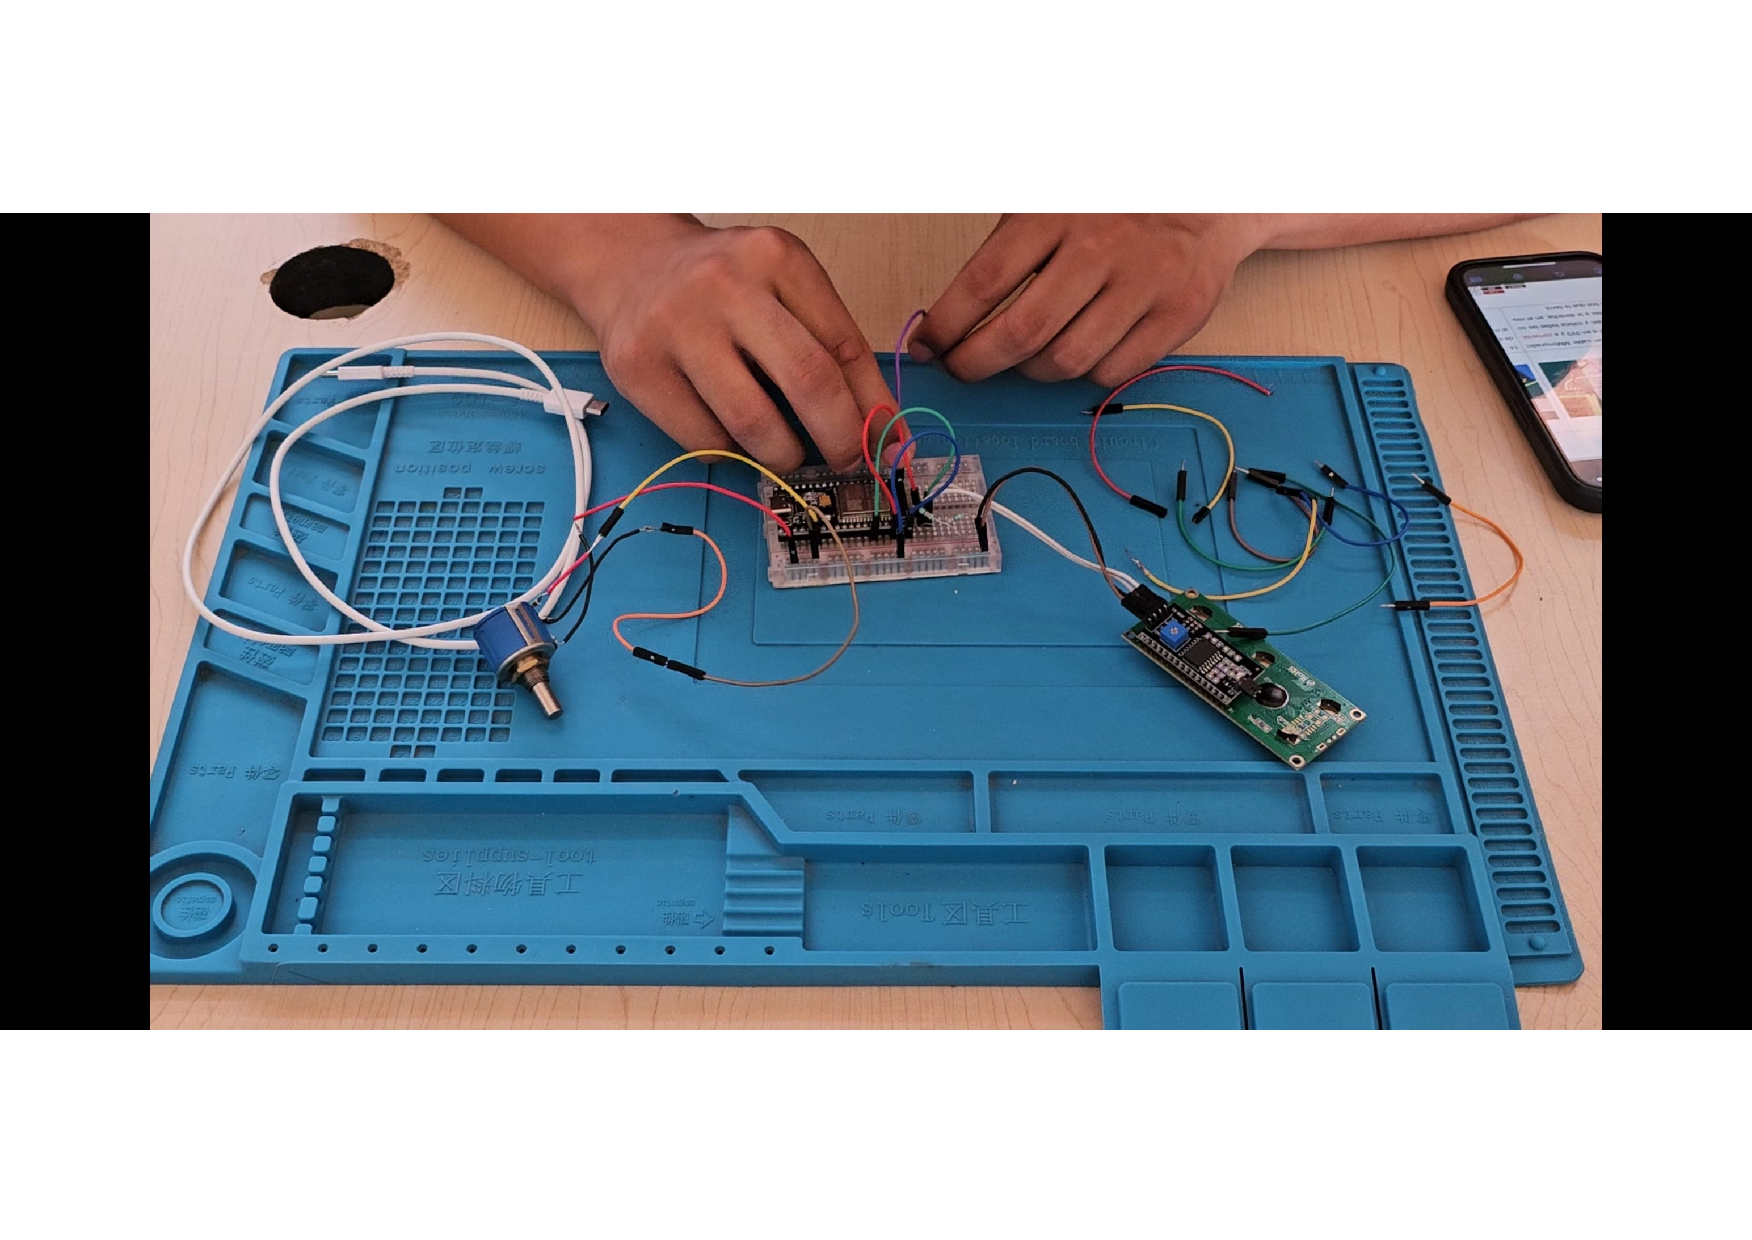
\includegraphics[trim = {25mm 25mm 25mm 10mm},clip,scale=0.3]{22/Img/ev3.pdf}
        \caption{Conexiones restantes}
        \label{fig:ev3}
    \end{figure}
    
    
    
    
    \begin{figure}[H]
        \centering
        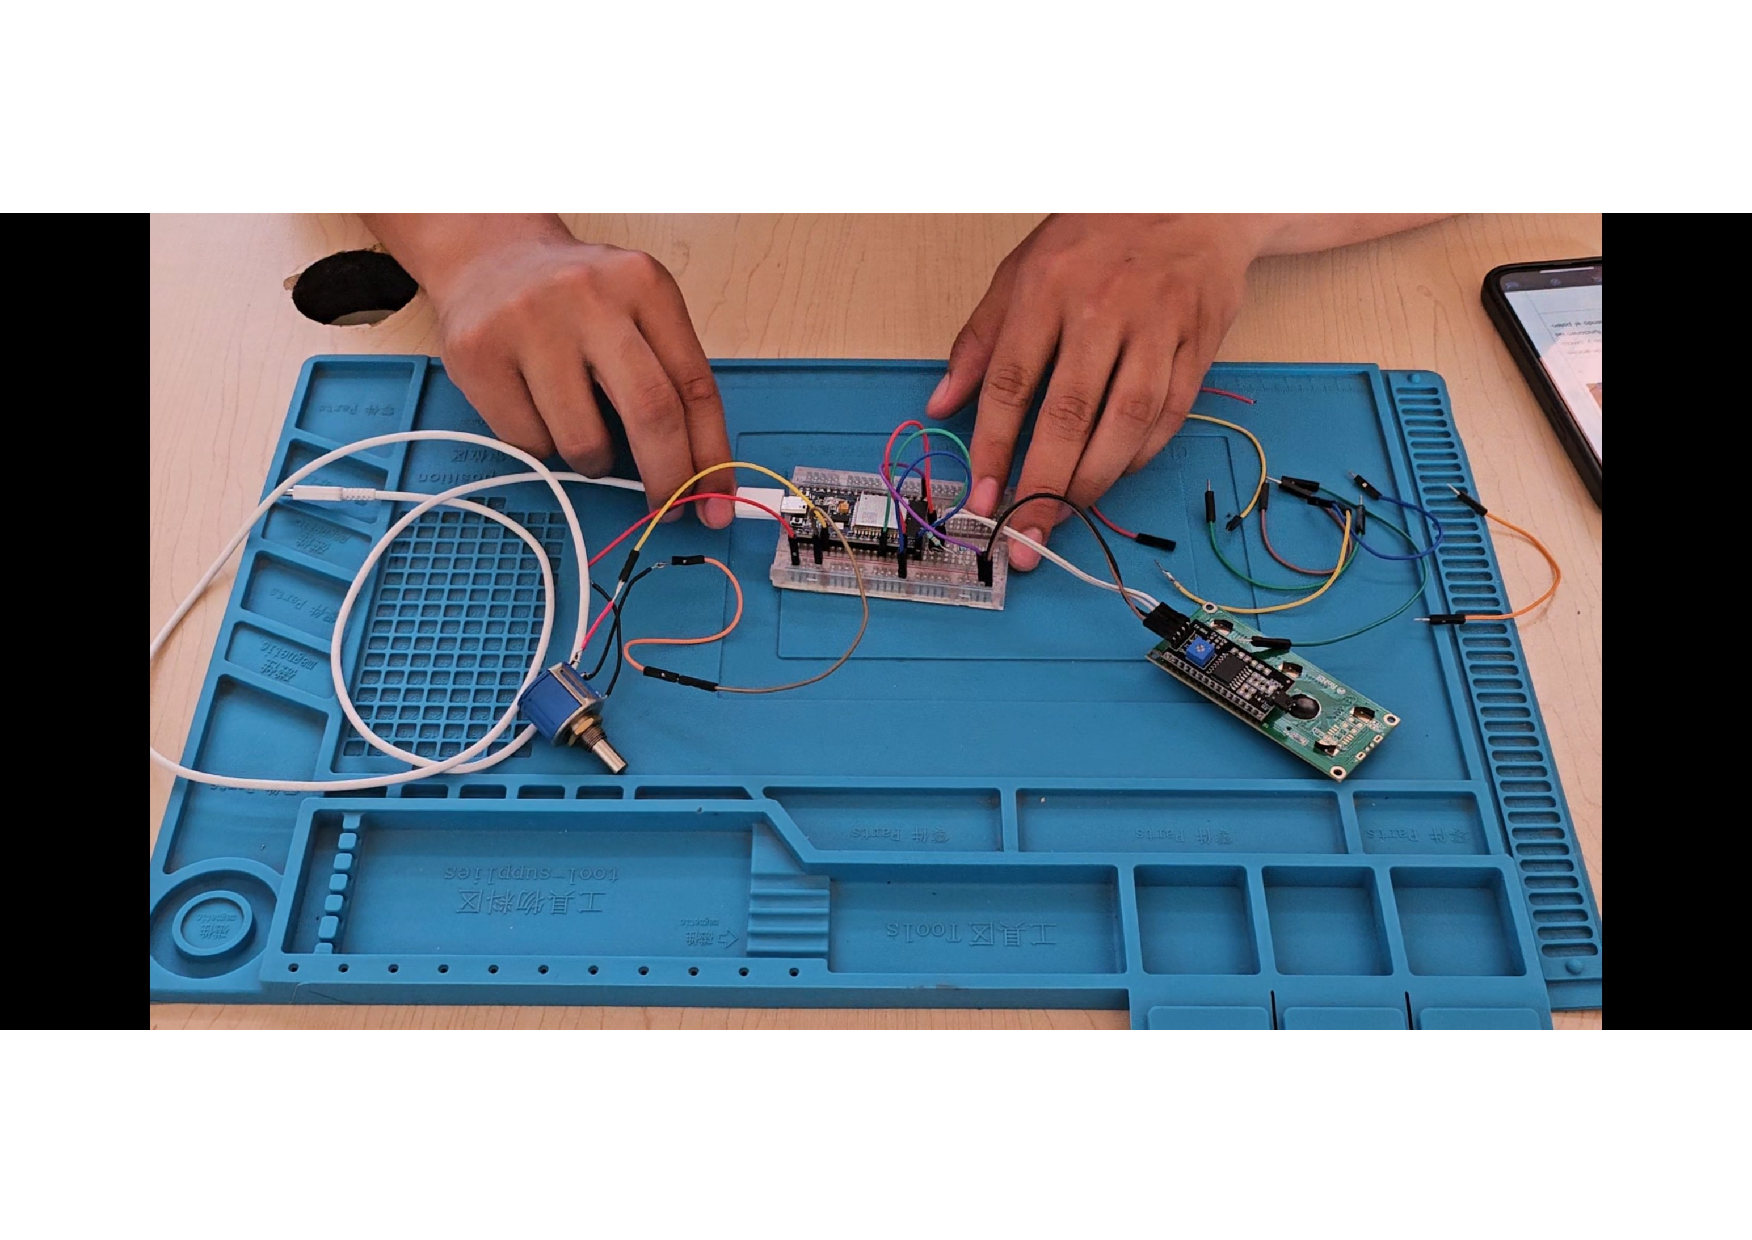
\includegraphics[trim = {25mm 25mm 25mm 10mm},clip,scale=0.3]{22/Img/ev4.pdf}
        \caption{Colocación el cable tipo C}
        \label{fig:ev4}
    \end{figure}
    
    
    \begin{figure}[H]
        \centering
        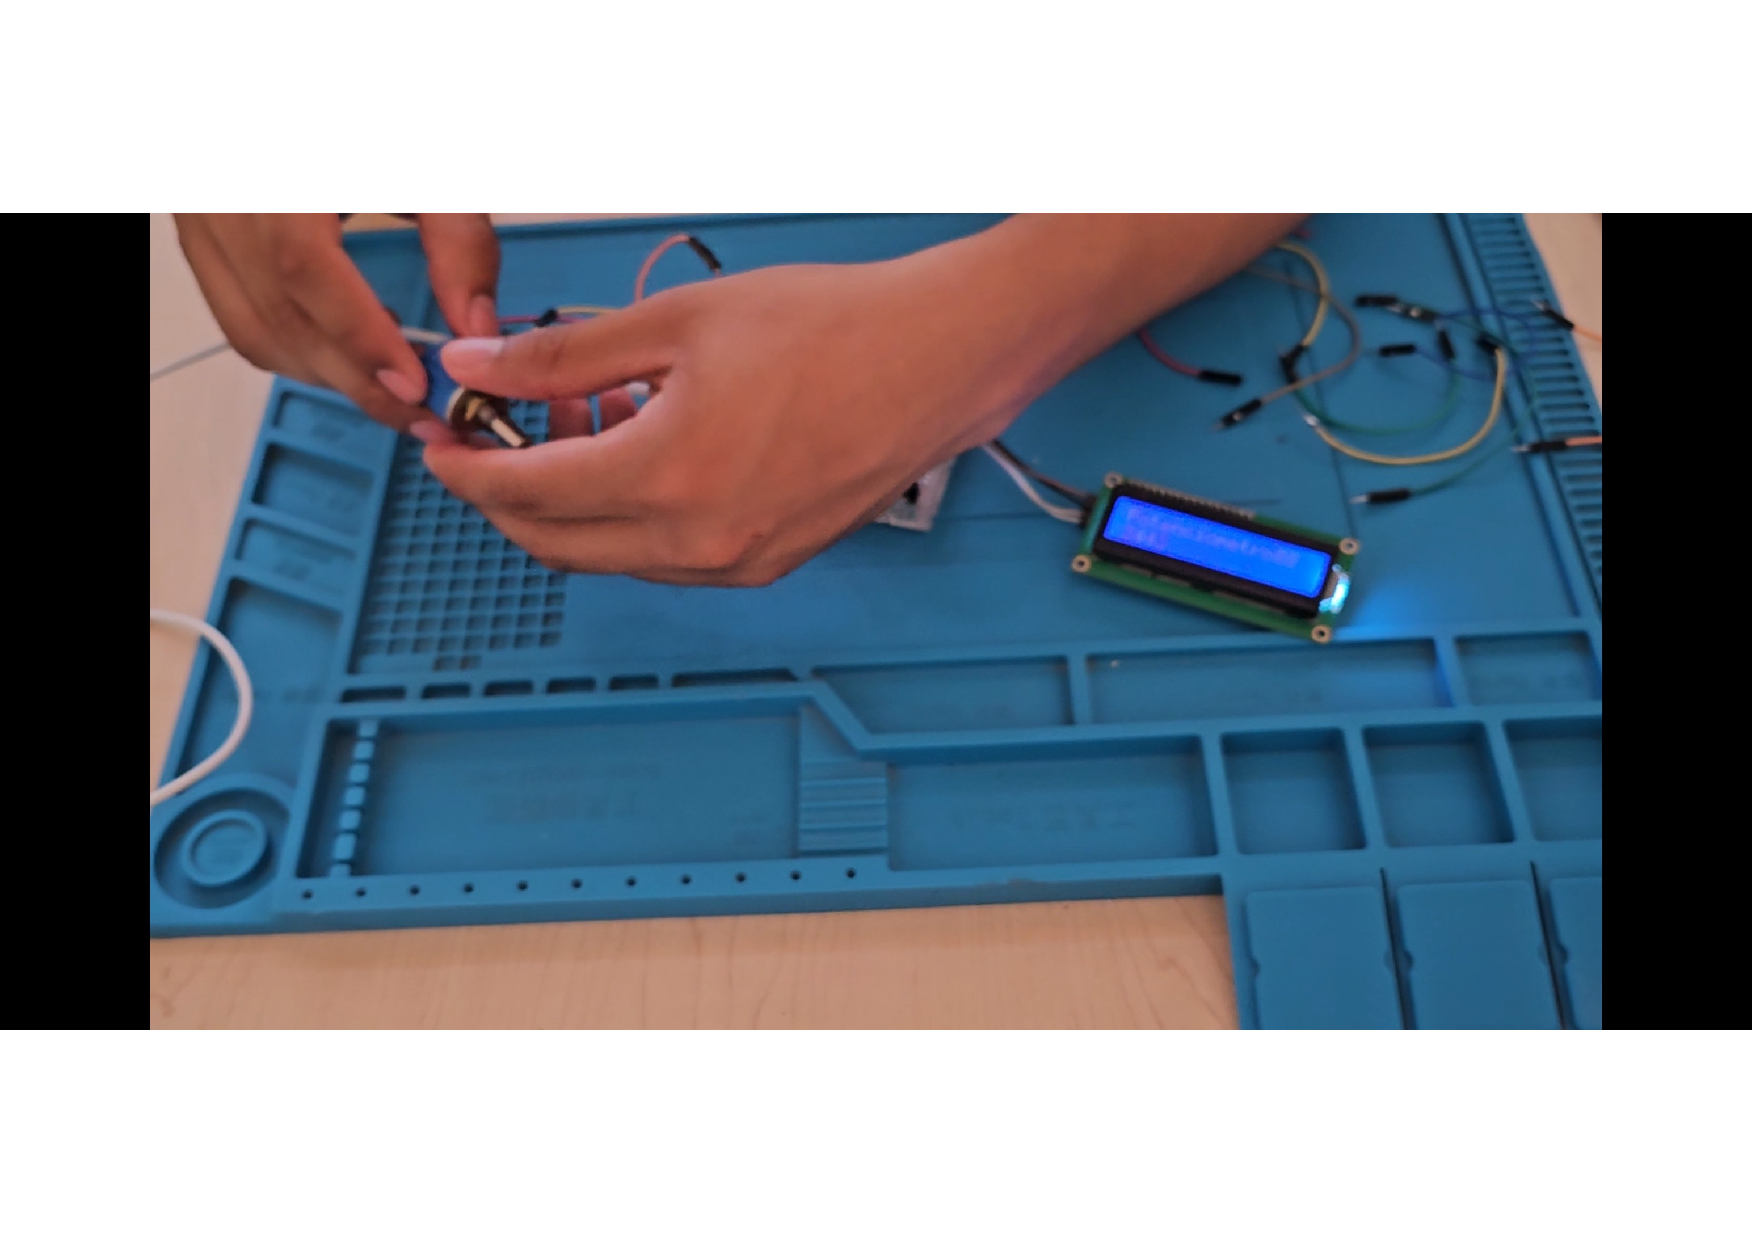
\includegraphics[trim ={25mm 25mm 25mm 10mm},clip,scale=0.3]{22/Img/ev5.pdf}
        \caption{Cambio de los valores con el potenciómetro}
        \label{fig:ev5}
    \end{figure}
    
    \begin{figure}[H]
        \centering
        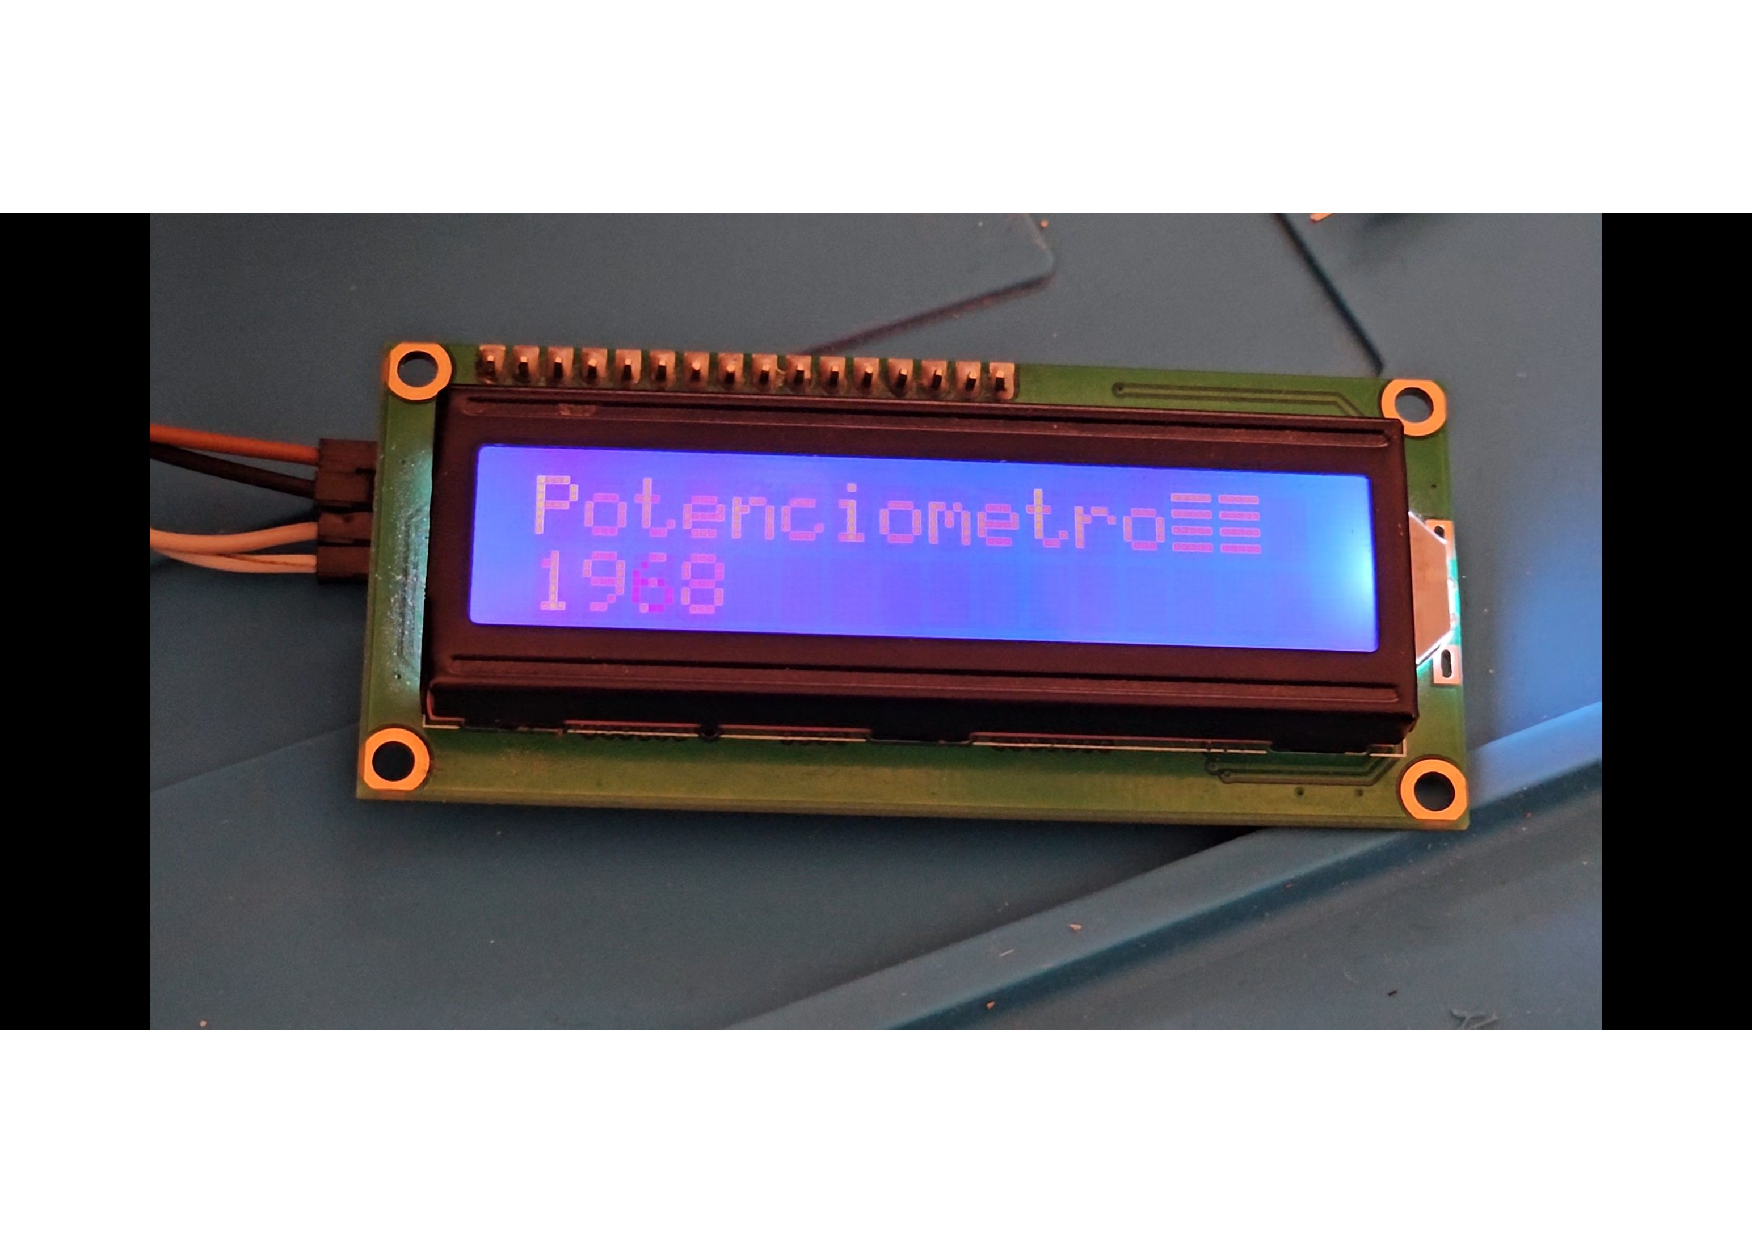
\includegraphics[trim = {25mm 25mm 25mm 10mm},clip,scale=0.3]{22/Img/ev6.pdf}
        \caption{Acercamiento a la LCD en funcionamiento}
        \label{fig:ev6}
    \end{figure}
    
    
    \begin{figure}[H]
        \centering
        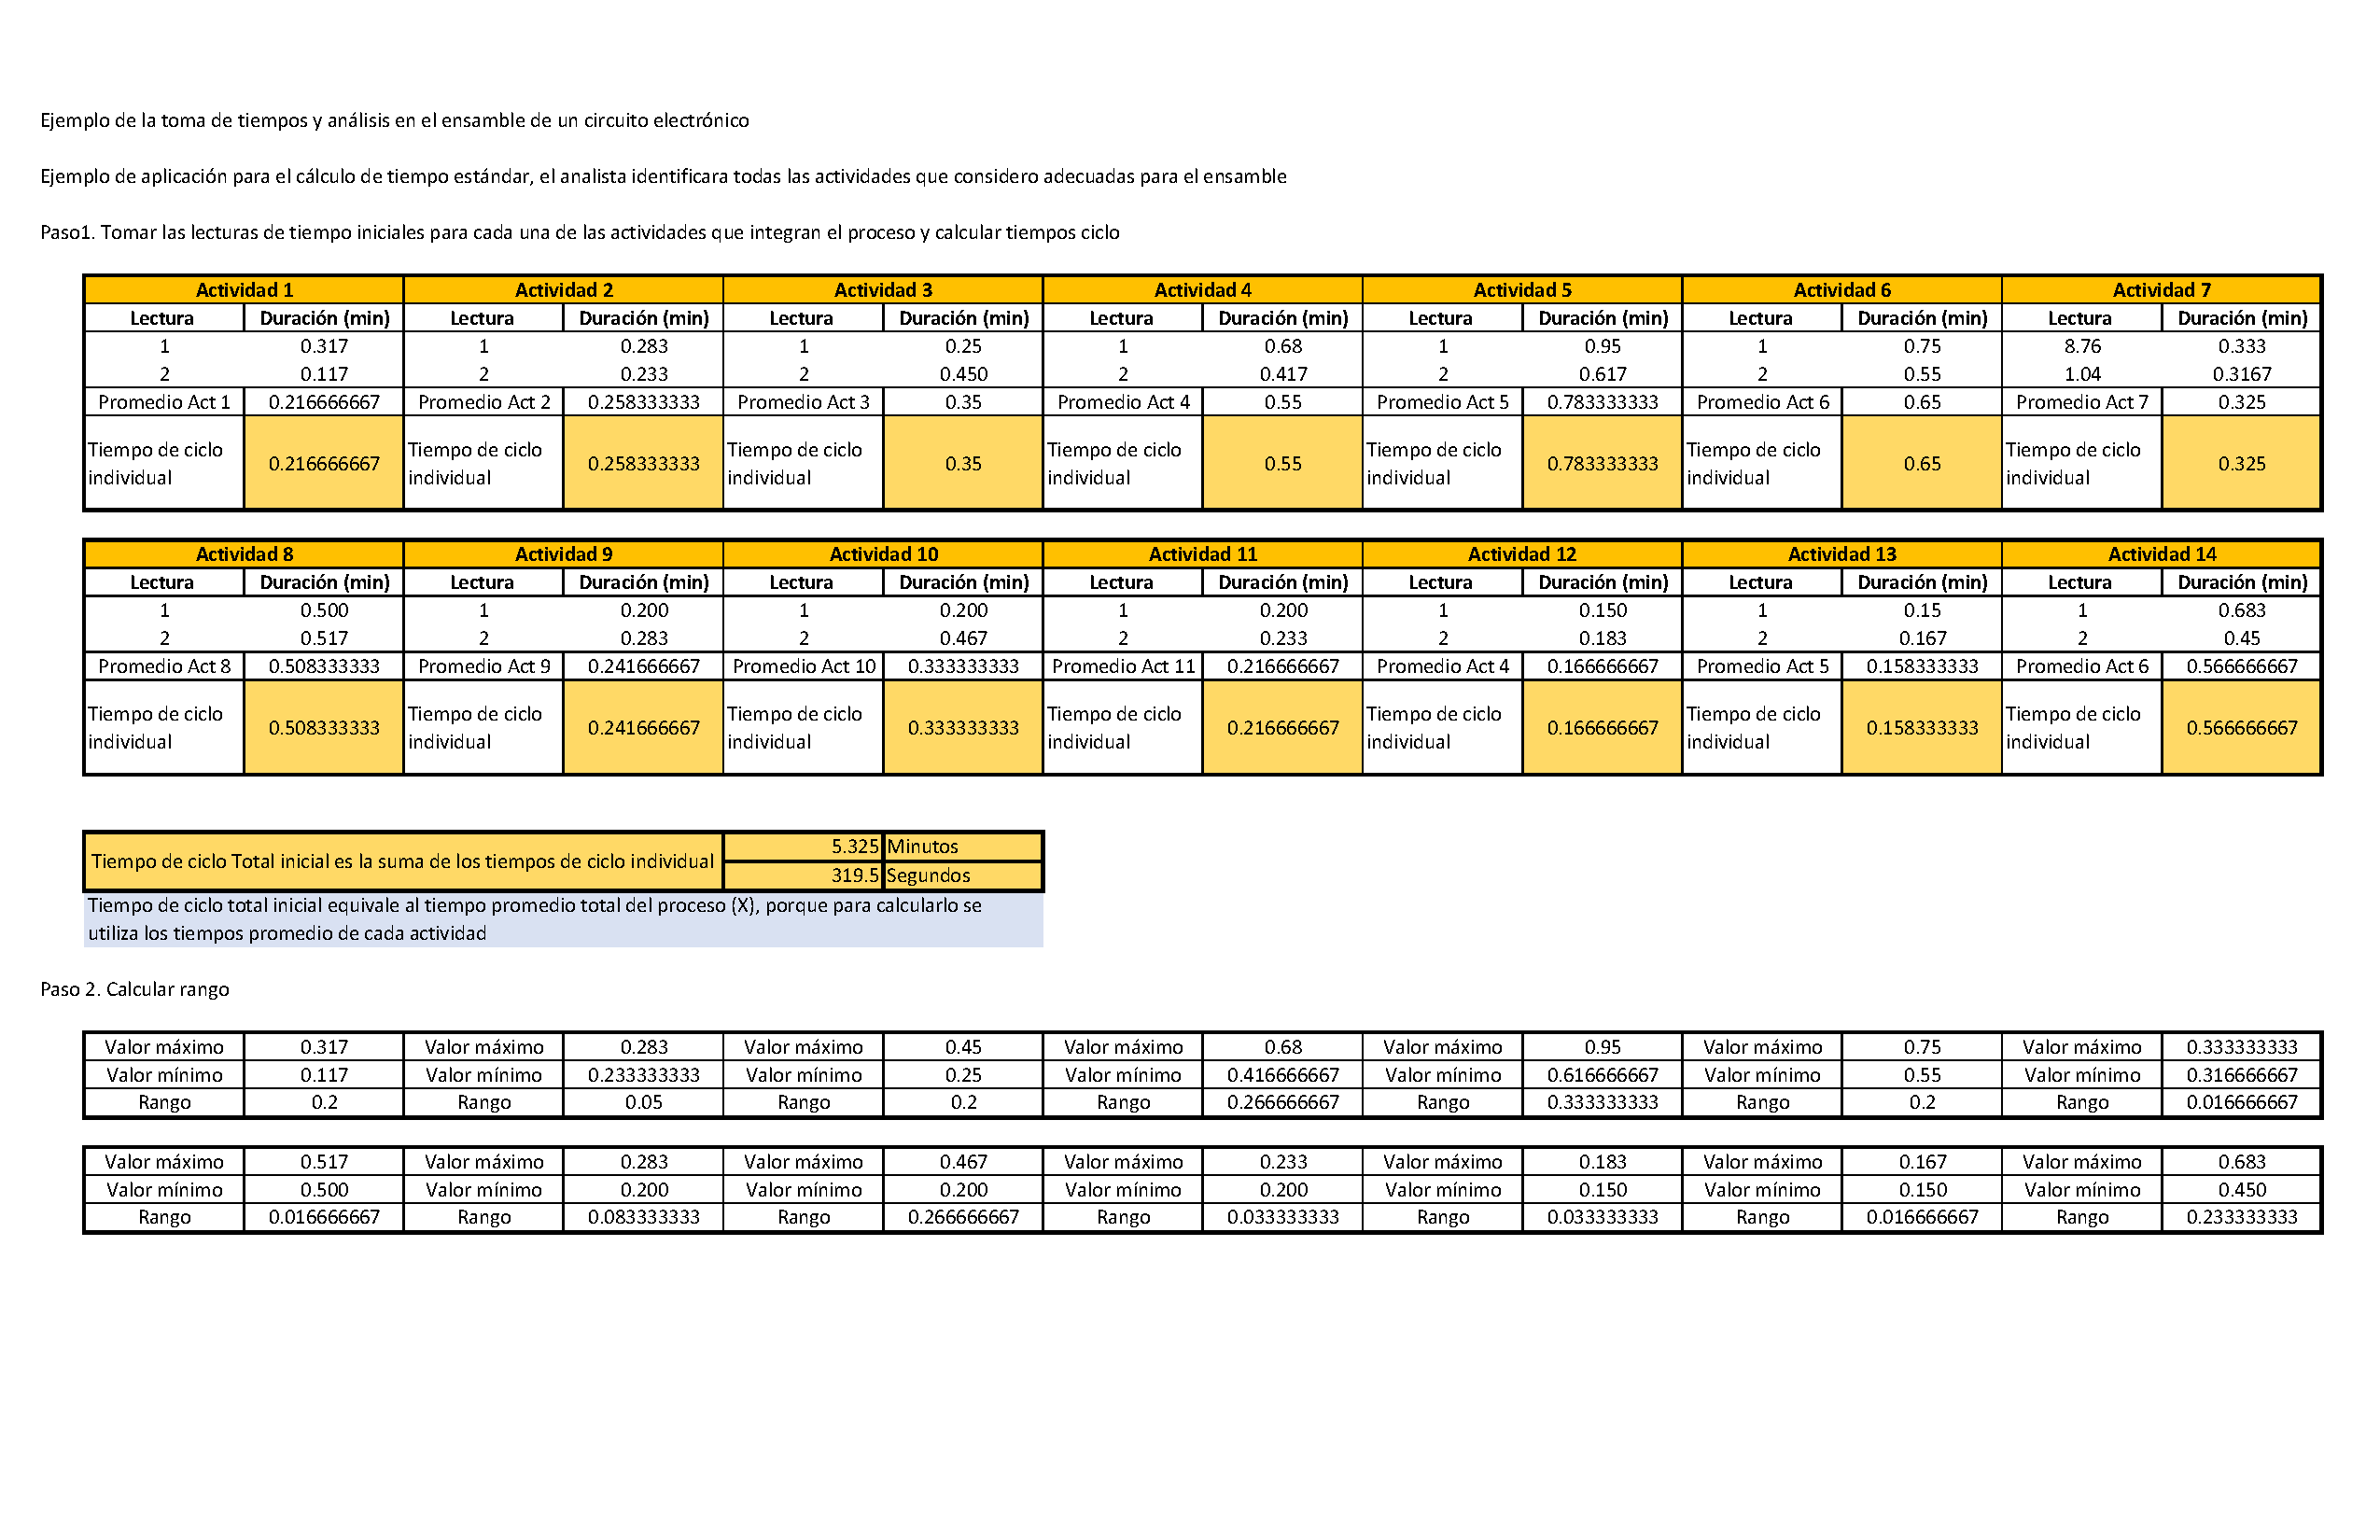
\includegraphics[trim = {6.4mm 50mm 6.4mm 19mm},clip,scale=0.3]{22/Img/tiempoCicloEnsamble.pdf}
        \caption{Hoja de datos y cálculo del tiempo ciclo}
        \label{fig:tiempoCiclo}
    \end{figure}
    
    
    
    
    \subsubsection{Corrección por balanceo de procesos}
    % 
    % 
    \subsubsection{Datos estándar, continuos y discretos}
    % 
    % 
    \subsection{Diseño de la forma más económica de realizar el trabajo}
    
    % 
    % 
    \subsection{Normalización de los métodos, materiales, herramientas e instalaciones}
    
    % 
    % 
    \subsection{Determinación del tiempo estándar para que una persona competente realice el trabajo con marcha normal}
    
    
    
    
    \subsection{Autores y Afiliaciones}
    
    \subsection{Tablas y Figuras}
    
    \section{Conclusiones}
    
    
    
    \section{Agradecimientos}
    
    
    \section{Referencias}
    
    
    
    
    % \newpage
    % \bibliographystyle{ieeetr}
    % \bibliography{22/referencias}
    % 
    % 
    %%%%%%%%%%%%%%%%%%%%%%%%%%%%%%%%%%
    \appendix
    %%%%%%%%%%%%%%%%%%%%%%%%%%%%%%%%%%
    % 
    \centering{\section[\appendixautorefname{}]{Apéndice Instructivo}}\label{Figura:instructivo}
    \includepdf[pages=2-5 ]{22/Img/instructivoMateriales.pdf}
    %%%%%%%%%%%%%%%%%%%%%%%%%%%%%%%%%%%%%%%%
    % 
    \centering{\section[\appendixautorefname{}]{Apéndice Materiales}}\label{Figura:Materiales}
    \includepdf[pages=6-7,]{22/Img/instructivoMateriales.pdf}
    % 
    %%%%%%%%%%%%%%%%%%%%%%%%%%%%%%%%%%%%%%%%
    \centering{\section[\appendixautorefname{}]{Apéndice de Diagrama Bimanual}}\label{Figura: DigBim}
    \includepdf[pages=-,]{22/Img/diagramaBimanual.pdf}
    
    %%%%%%%%%%%%%%%%%%%%%%%%%%%%%%%%%%%%%%%%
    \centering{\section[\appendixautorefname{}]{Apéndice de Tablas MTM}}\label{Figura:TablasMTM}
    \includepdf[pages=-,]{22/Img/tablasMTM.pdf}
    
    \newpage
    \bibliographystyle{ieeetr}
    \bibliography{22/referencias}